\documentclass[12pt, oneside]{book} % Drop `oneside' if difference between even and odd pages is to be considered.

% Bibliography style

\bibliographystyle{alpha}

\usepackage{amsthm}
\usepackage[doublespacing]{setspace}
\usepackage[top=1in, bottom=1in, left=1.25in, right=1.25in]{geometry}
\usepackage{fancyhdr}
\usepackage[all]{xy}
\usepackage{enumitem}
\usepackage{color}
\usepackage{amssymb}
\usepackage{amsmath}
\usepackage{subcaption}
\captionsetup[subfigure]{labelfont=rm}
\usepackage{etoolbox}
\usepackage{tikz-cd}
\usepackage{graphicx}
\usepackage{float}
\graphicspath{{"./figures/"}} % Path for figures
\usepackage{hyperref}
\hypersetup{colorlinks=true,allcolors=blue}

\newcommand{\SmallHack}[1]{\lowercase{#1}}
\newcommand{\Bibkeyhack}[3]{}

% Custom commands

\newcommand{\N}{\mathbb{N}}
\newcommand{\Z}{\mathbb{Z}}
\newcommand{\Q}{\mathbb{Q}}
\newcommand{\R}{\mathbb{R}}
\newcommand{\C}{\mathbb{C}}
\newcommand{\Ell}{\mathcal{L}}
\newcommand{\Err}{\mathcal{R}}
\newcommand{\Eff}{\mathcal{F}}
\newcommand{\Mu}{\text{M}}
\newcommand{\rk}{\mathrm{rk}}
\newcommand{\im}{\mathrm{Im}}
\newcommand{\id}{\mathrm{id}}
\newcommand{\aut}{\mathrm{Aut}}
\newcommand{\inn}{\mathrm{int}}
\newcommand{\tilx}{\widetilde{X}}
\newcommand{\tily}{\widetilde{Y}}
\newcommand{\tilya}{\widetilde{Y_{1}}}
\newcommand{\tilyb}{\widetilde{Y_{2}}}
\newcommand{\tilyi}{\widetilde{Y_{i}}}
\newcommand{\tilw}{\widetilde{W}}
\newcommand{\chileq}{\leq_{\chi}}
\newcommand{\pia}{\pi_{1}(Y_{1})}
\newcommand{\pib}{\pi_{1}(Y_{2})}
\newcommand{\pii}{\pi_{1}(Y_{i})}
\newcommand{\piw}{\pi_{1}(W)}
\newcommand{\piwa}{\pi_{1}(W_{1})}
\newcommand{\piwb}{\pi_{1}(W_{2})}
\newcommand{\piwi}{\pi_{1}(W_{i})}
\newcommand{\pibarw}{\pi_{1}(\barw)}
\newcommand{\pix}{\pi_{1}(X)}
\newcommand{\piy}{\pi_{1}(Y)}
\newcommand{\dplu}{\partial_{+}}
\newcommand{\dmin}{\partial_{-}}
\newcommand{\dhor}{\partial_{h}}
\newcommand{\dver}{\partial_{v}}
\newcommand{\dpm}{\partial_{\pm}}
\newcommand{\wgamm}{W_{\Gamma}}
\newcommand{\ydel}{Y_{\Delta}}
\newcommand{\pgamm}{p_{\Gamma}}
\newcommand{\tilf}{\widetilde{f}}
\newcommand{\barx}{\overline{X}}
\newcommand{\barp}{\overline{p}}
\newcommand{\barw}{\overline{W}}
\newcommand{\tilgamma}{\widetilde{\gamma}}
\newcommand{\pmin}{p_{-}}
\newcommand{\pplu}{p_{+}}
\newcommand{\ppm}{p_{\pm}}
\newcommand{\pdel}{p_{\Delta}}
\newcommand{\rna}{R_{n}(Y_{1})}
\newcommand{\rnb}{R_{n}(Y_{2})}
\newcommand{\rnw}{R_{n}(W)}
\newcommand{\son}{\mathrm{SO}(n)}
\newcommand{\coker}{\mathrm{coker}}
\newcommand{\disc}{\mathrm{disc}}
\newcommand{\spin}{\text{Spin}}
\newcommand{\spinc}{\text{Spin}^{c}}
\newcommand{\Rn}[1]{\uppercase{\romannumeral #1}}
\newcommand{\RN}[1]{\uppercase{\romannumeral #1}}
\newcommand{\rn}[1]{\romannumeral #1}

% Custom environments

\theoremstyle{definition}
%\newtheorem{theorem}{Theorem}[section]
\newtheorem{theorem}{Theorem}
\newtheorem{definition}[theorem]{Definition}
\newtheorem{lemma}[theorem]{Lemma}
\newtheorem{corollary}[theorem]{Corollary}
\newtheorem{proposition}[theorem]{Proposition}
\newtheorem{conjecture}[theorem]{Conjecture}
\newtheorem{example}[theorem]{Example}
\newtheorem{xca}[theorem]{Exercise}
\newtheorem{question}[theorem]{Question}
\newtheorem*{question*}{Question}

\theoremstyle{remark}
\newtheorem{remark}[theorem]{Remark}
\newtheorem{remarks}[theorem]{Remarks}
\newtheorem*{remark*}{Remark}
\newtheorem*{remarks*}{Remarks}

\newcommand{\thesistitle}{Grothendieck maps associated to braids and their Khovanov-Rozansky homologies} % Thesis title
\newcommand{\thesistitlecaps}{GROTHENDIECK MAPS ASSOCIATED TO BRAIDS AND THEIR KHOVANOV-ROZANSKY HOMOLOGIES} % Capitalized thesis title


%%%%%%%%%%%%%%%%%%%%%%%%%%%%%%%%%%%%%%%%%%%%%%%%%%%%%%%%%%%%%%%%%%%%%%%%%%%%%%%%%%%%%%%%

% Title page information

\font\titlefont=cmr12 at 24pt
\title{\vspace{-1.5in}
{\titlefont \thesistitlecaps}}
\font\authorfont=cmr12 at 16 pt
\author{{\authorfont Jee Uhn Kim}}
\date{
\vspace{1.25in}
A dissertation submitted to the Faculty of the\\
Department of Mathematics in partial fulfillment of the\\
requirements for the degree of Doctor of Philosophy\\
\vspace{1.25in}
%
{
\setstretch{1}
Boston College \\
Morrissey College of Arts and Sciences \\
Graduate School\\
}
\vspace{.25in}
%
May 2025
}

%%%%%%%%%%%%%%%%%%%%%%%%%%%%%%%%%%%%%%%%%%%%%%%%%%%%%%%%%%%%%%%%%%%%%%%%%%%%%%%%%%%%%%%%

% Header settings

% \makeatletter
% \newcommand{\rightorleftmark}{%
%   \begingroup\protected@edef\x{\rightmark}%
%   \ifx\x\@empty
%     \endgroup\leftmark
%   \else
%     \endgroup\rightmark
%   \fi}
% \makeatother

\pagestyle{fancy}
    \renewcommand{\headrulewidth}{0.1pt}
    \lhead{}
    \rhead{}
    \chead{\fontsize{9}{12}\selectfont\nouppercase{\rightmark}}
    \cfoot{\thepage}

%%%%%%%%%%%%%%%%%%%%%%%%%%%%%%%%%%%%%%%%%%%%%%%%%%%%%%%%%%%%%%%%%%%%%%%%%%%%%%%%%%%%%%%%

\begin{document}

% Title page
\maketitle

\newpage

% Copyright page
\thispagestyle{empty}
\begin{center}
\null
\vfill
\textcopyright 2025 Jee Uhn Kim
\end{center}

\newpage

% Title and abstract page
\thispagestyle{empty}
\begin{center}
{\bf \thesistitle}\\
Jee Uhn Kim\\
Advisor: David Treumann, Ph.D.
\end{center}

Abstract

\frontmatter % Roman page numbering starts here

% Table of contents
\thispagestyle{plain}
\phantomsection
\addcontentsline{toc}{chapter}{Contents}
%\chead{}
\cfoot{\thepage}
\tableofcontents

\newpage

% List of figures
\thispagestyle{plain}
\phantomsection
\addcontentsline{toc}{chapter}{List of Figures}
\cfoot{\thepage}
\listoffigures

\newpage

% Acknowledgments
\thispagestyle{plain}
\phantomsection
\addcontentsline{toc}{chapter}{Acknowledgements}
\cfoot{\thepage}
\vspace*{0.75in}
{\Large\textbf{Acknowledgments}}
\
\
\noindent

Acknowledgements

\newpage

\mainmatter % Standard page numbering starts here

%%%%%%%%%%%%%%%%%%%%%%%%%%%%%%%%%%%%%%%%%%%%%%%%%%%%%%%%%%%%%%%%%%%%%%%%%%%%%%%%%%%%%%%%
%%%%%%%%%%%%%%%%%%%%%%%%%%%%%%%%%%%%%%%%%%%%%%%%%%%%%%%%%%%%%%%%%%%%%%%%%%%%%%%%%%%%%%%%

\chapter{Introduction}\label{chapter_introduction}

\section{Background and context}\label{sec_background_and_context}

\subsection*{Contact Geometry}
First, we review basics of contact geometry, see \cite{etnyre2005legendrian}\cite{geiges2008introduction} for details. A contact structure on a $(2n-1)$-dimensional manifold $X$ is a maximally nonintegrable distribution of $(2n-2)$-planes. A contact structure defined globally as a kernel for a chosen $1$-form $\alpha$ is said to be co-oriented and $\alpha$ is said to be its co-orientation. An $(n-1)$-dimensional submanifold $\Lambda \subset X$ is said to be Legendrian if its tangent bundle is contained in the contact hyperplanes. Now let's look at several examples of contact manifolds.
\begin{enumerate}[label = (\arabic*)]
\item the contagent bundle $T^*M$ of a manifold $M$ carries a canonical $1$-form which is in local coordinates $(q_i,p_i)$, $\theta := \underset{i}{\sum} p_i dq_i$. This form is invariant under dialation in cotangent directions, therefore, $\theta$ descends to a well-defined $1$-form(unique up to positive scalar function) on the cosphere bundle $T^\infty M := (T^*M - 0_M)/\R_+$ where $0_M$ is the zero section and $\R_+$-action is the dialation action along cotangent directions. Therefore, $T^\infty M$ is equipped with a natural contact structure.

\item $\R^3_{x,y,z}$ with the global $1$-form $\alpha = dz - ydx$ defines a co-oriented contact structure. We can embed $\R^3_{x,y,z}$ in $T^{\infty,-}\R^2_{x,z}$ as an open contact submanifold as follows:
\begin{align*}
\R^3_{x,y,z} &\rightarrow \R^2_{x,z} \times S^1 \\
(x,y,z) & \mapsto (x,z;y,-1)
\end{align*}
The image is the contact submanifold $T^{\infty,-}\R^2_{x,z}$ of "downward" covectors.

\item Note that construction $(2)$ is invariant under translation $x \mapsto x+1$. Let $S^1_x := \R_x / \Z$, then standard $1$-form $dz - ydx$ descends to $S^1_x \times \R_{y,z}$ and it embeds as the contact submanifold $T^{\infty, -}(S^1_x \times \R_z)$ in $T^\infty(S^1_x \times \R_z)\cong S^1_x \times \R_z \times S^1_y$. The``cocircle bundle" in the title of the thesis refers to $T^\infty (S^1_x \times \R_z)$.
\end{enumerate}

\subsection*{Front Projection}
Now let's restrict our attention to the case when the base manifold $M$ is either $\R^2_{x,z}$ or $S^1_x \times \R_z$. We call the map $\pi : T^\infty M \rightarrow M$ the "front projection" and $\pi(\Lambda)$ the ``front diagram".
\begin{itemize}
\item when $M = \R^2_{x,z}$, $\pi : \R^3_{x,y,z} \subset T^\infty \R^2_{x,z} \rightarrow \R^2_{x,z}$ is the projection onto $x,z$ coordinates. We call $\R^2_{x,z}$ a front plane.

\item similarly, when $M = S^1_x \times \R_{z}$, $\pi : S^1_x \times \R^2_{y,z} \subset T^\infty (S^1_x \times \R_{z}) \rightarrow S^1_x \times \R_{z}$ is the projection onto $x,z$ coordinates. We call $S^1_x \times \R_{z}$ a front cylinder.
\end{itemize}
A Legendrian $\Lambda \subset T^{\infty}M$ at immersed points of $\pi(\Lambda)$can be recovered from $\pi(\Lambda)$ because $\Lambda$ vanishes on the contact form $dz-ydx$, we have $y = \frac{dz}{dx}$ as long as it is in general position. Under Hamiltonian isotopy, $\Lambda$ can be put in general position, i.e.
\begin{itemize}
\item $\pi|_\Lambda$ is locally injective.

\item there are only finitely many points on $M$ at which $\pi(\Lambda)$ is not an embedded submanifold. These are either
\begin{itemize}
\item cusps where $\pi|_{\Lambda}$ is injective and $\frac{dz}{dx}$ has a well-defined limit of $0$.

\item crossing where $\pi(\Lambda)$ is locally a transverse intersection of two smooth curves.
\end{itemize}
\end{itemize}
In this paper, we only allow $\pi(\Lambda)$ to have crossings. We won't consider $\pi(\Lambda)$ with cusps. There are no interesting examples in $\R^3_{x,y,z}$ but there are many interesting ones in the cocircle bundle of a cylinder.
Suppose we have a smooth parametrized curve $\Phi$ in $M$
\begin{itemize}
\item which is an immersion

\item which has finitely many self-intersections and they are transverse.
\end{itemize}
and a choice of preferred side, i.e. a co-orientation, diagramatically described using hairs normal to the $\Phi$ pointing the preferred direction. We say that the region on the preferred side lies beneath the  the arc and the region on the other side lies above the arc. We can lift it to a Legendrian in $T^{\infty}M$. Therefore, the Legendrian in $T^{\infty}M$ amounts to the datum of the co-oriented front diagram.

\subsection*{Constructible sheaves}
Let $M$ be a manifold and $\mathcal{S}$ Whitney a stratification of $M$. A sheaf of $\C$-vector space $\mathscr{F}$ on $M$ is $\mathcal{S}$-constructible if the restriction of $\mathscr{F}$ to each stratum of $s\in \mathcal{S}$, $\mathscr{F}|_s$, is a locally constant sheaf. $\mathscr{F}$ is called constructible if there exists a Whitney stratification $\mathcal{S}$ such that $\mathscr{F}$ is $\mathcal{S}$-constructible.
$Sh^\bullet_{naive}(M;\C)$ denotes the triangulated dg category whose objects are cochain complexes of sheaves of $\C$-vector spaces of bounded cohomology whose cohomology sheaves are constructible sheaves. If we localize $Sh^\bullet_{naive}(M;\C)$ with respect to acyclic complexes, in the sense of \cite{drinfeld2004dg}, we get $Sh^\bullet(M;\C)$. We denote $Sh^\bullet_{\mathcal{S}}(M;\C)$ the full subcategory of $Sh^\bullet (M;\C)$ of complexes whose cohomology sheaves are constructible with respect to $\mathcal{S}$. From now on we will call objects of $Sh^\bullet(M;\C)$ simply as sheaves.\\

\subsection*{Singular Support}
To each $\mathscr{F}\in Sh^\bullet (M;\C)$, we assign a closed conical subset $SS(\mathscr{F})\subset T^*M$, called the singular support of $\mathscr{F}$ following \cite{goresky1983stratified}\cite{schurmann2012topology}\cite{shende2017legendrian}. For more general treatment, see \cite{kashiwara2013sheaves}. Fix a Riemannian metric on $M$ and choose an $\epsilon$-ball $B_\epsilon(x)$ around a point $x\in M$. The following constructions are independent of the choice of metrics. Let $\mathscr{F}$ be an $\mathcal{S}$-constructible sheaf on $M$. Fix a point $x\in M$ and a smooth function $f$ on $B_\epsilon(x)$. For $\epsilon,\delta >0$, we define the local Morse group to be
\[
Mo_{x,f,\epsilon,\delta}(\mathscr{F}) := H^*(B_\epsilon(x)\cap f^{-1}((-\infty,f(x)+\delta)),B_\epsilon(x)\cap f^{-1}((-\infty,f(x)-\delta));\mathscr{F})
\]
For $\epsilon' < \epsilon$ and $\delta' < \delta$, there is a canonical restriction map
\[
Mo_{x,f,\epsilon,\delta}(\mathscr{F})\rightarrow Mo_{x,f,\epsilon',\delta'}(\mathscr{F})
\]
The above restriction is an isomorphism if $\epsilon$ and $\delta$ are sufficiently small and $f$ is stratified Morse at $x$. This allows us to define $Mo_{x,f}(\mathscr{F})$ for $f$ suitably generic with respect to $\mathcal{S}$\cite[Prop.~7.5.3]{kashiwara2013sheaves}. In fact, $Mo_{x,f} (\mathscr{F})$ depends only on the Hessian of $f$ at $x$.
Let $\mathscr{F}\in Sh^\bullet (M;\C)$, then $(x,\xi)\in T^*M$ is characteristic with respect to $\mathscr{F}$ if for some stratified Morse function $f$ with $df_x = \xi$, the local Morse group $Mo_{x,f}(\mathscr{F})$ is nonzero. Then we define the singular support of $\mathscr{F}$ to be the closure of the set of characteristic covectors for $\mathscr{F}$ in $T^*M$. Singular support is a conic Lagrangian i.e. stable under $\R_+$-dialation along contangent fibers.\\
Fix a conic Lagrangian $L\subset T^*M$, then we define $Sh^\bullet_L(M;\C)$ to be the full subcategory of $Sh^\bullet_L(M;\C)$ whose objects are sheaves singular supported in $L$. If $\Lambda\subset T^\infty M$ is a Legendrian, then we define $Sh^\bullet_\Lambda(M;\C) := Sh^\bullet_{\R_+ \Lambda \cup 0_M}(M;\C)$ where $0_M \subset T^*M$ is the zero section.

\subsection*{Combinatorial Model of $Sh^\bullet_\Lambda(M;\C)$}
The first necessary condition for $\mathscr{F}\in Sh^\bullet(M;\C)$ to belong to $Sh^\bullet_L(M;\C)$ is that $\mathscr{F}$ is constructible with respect to the stratification on $M$ induced by the front projection of $\Lambda$. That is the Whitney stratification whose zero dimensional strata are crossings, one dimensional strata are the arcs of $\pi(\Lambda)$ between crossings and two dimensional strata are the connected components of the complement of $\pi(\Lambda)$ in $M$.

\begin{definition}
Given a stratification $\mathcal{S}$, the star of a stratum $s\in \mathcal{S}$ is the union of strata that contain $s$ in their closure. We view $\mathcal{S}$ as a poset category $s\leq t$ if and only if $s \subset \overline{t}$. We call the map from $s$ to $t$ as a generization map. We say $\mathcal{S}$ is a regular cell complex if every stratum is contractible and moreover the star of each stratum is contractible.
\end{definition}

\begin{definition}
We define $Fun^\bullet_{naive}(\mathcal{S},\C)$ to be the dg category of functors from $\mathcal{S}$ to the category whose objects are cochain complexes of $\C$-vector spaces and whose maps are cochain maps. 
We define $Fun^\bullet(\mathcal{S}, \C)$ the dg quotient \cite{drinfeld2004dg} of $Fun^\bullet_{naive}(\mathcal{S},\C)$ by the thick subcategory of functors taking values in acyclic complexes.
\end{definition}

\begin{proposition}\label{KS}
\cite{kashiwara1984riemann}, \cite{shepard1985cellular}, \cite[Lemma~2.3.2]{nadler2009microlocal}.Let $\mathcal{S}$ be a Whitney stratification of $M$. Consider the functor 
\begin{align*}
&\Gamma_\mathcal{S} : Sh^\bullet_\mathcal{S}(M;\C) \rightarrow Fun^\bullet(\mathcal{S},\C)\\
&\mathscr{F} \mapsto [s\mapsto \Gamma(star(s);\mathscr{F})]
\end{align*}
If $\mathcal{S}$ is a regular cell complex, then $\Gamma_\mathcal{S}$ is a quasi-equivalence.
\end{proposition}
However, the stratification induced by the front diagram is not necessarily a regular cell complex. Therefore, we choose an $\mathcal{S}$ that refines of the stratification induced by $\pi(\Lambda)$. In figures, we draw the new line segments in squiggly lines. \\
The restriction of $\Gamma_\mathcal{S}$ to $Sh^\bullet_\Lambda(M;\C)$ is quasi-fully faithful. We will describe the essential image of $Sh^\bullet_\Lambda(M;\C)$ under $\Gamma_\mathcal{S}$.

\begin{definition}
Let $\mathcal{S}$ be a regular cell complex refining the stratification induced by the front diagram. we define $Fun^\bullet_\Lambda(\mathcal{S},\C)$ to be the full subcategory of $Fun^\bullet(\mathcal{S},\C)$ whose objects satisfy the following properties.
\begin{itemize}
\item every map from a zero dimensional stratum in $\mathcal{S}$ which is not a crossing is sent to quasi-isomorphism.

\item every map from a one dimensional stratum which is not contained in an arc is sent to quasi-isomorphism.

\item for each crossing $c\in \mathcal{S}$, Let $N$, $E$, $S$, $W$ be the north, east, south, and west regions adjoining $c$, and let $nw$, $ne$, $sw$, $se$ be the arcs separating them.
\begin{figure}[H] 
    \centering
    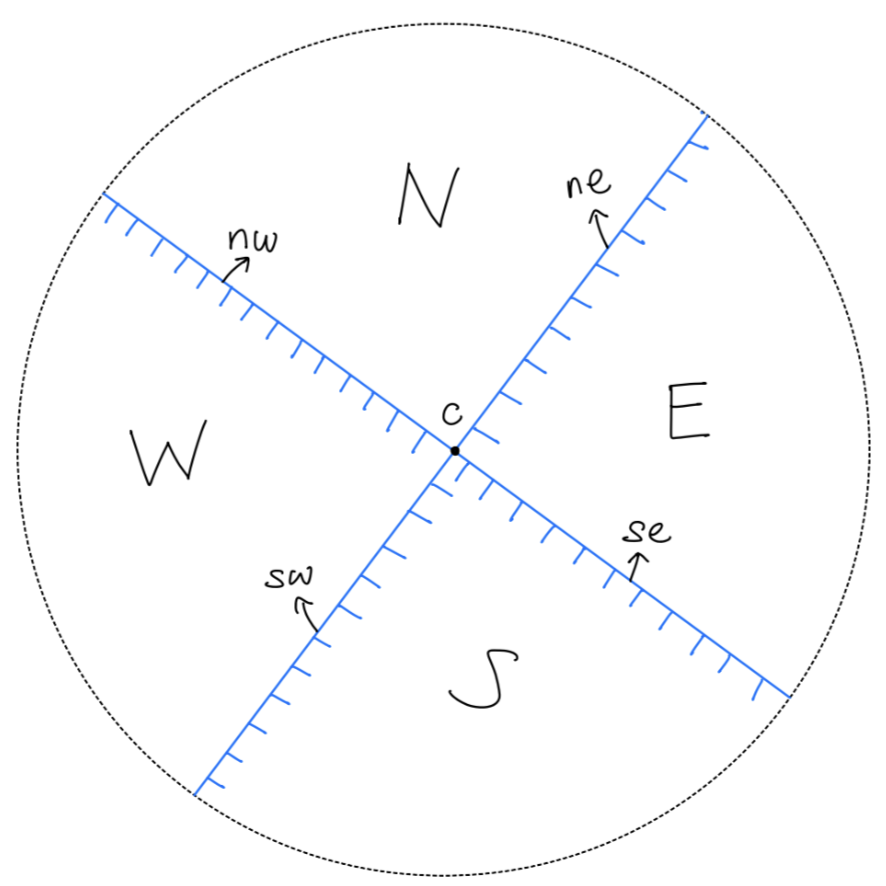
\includegraphics[scale = 0.55]{diagrams/intro/1.png}
    \caption{}
    \label{fig:your-label}
\end{figure}
Then the following maps are sent to quasi-isomorphisms.
\begin{itemize}
\item maps between $c$, $sw$, $se$, and $S$.
\item a map from $nw$ to $W$.
\item a map from $ne$ to $E$.
\end{itemize}

\item for each crossing $c\in \mathcal{S}$, we restrict the poset structure to the strata containing $c$ in its closure, we get
\[
\begin{tikzcd}
& & N & &\\
& nw\arrow[ur]\arrow[dl] & & ne\arrow[ul]\arrow[dr] &  \\
W& & c\arrow[uu]\arrow[dd]\arrow[ll]\arrow[rr]\arrow[ul]\arrow[ur]\arrow[dl]\arrow[dr] & & E \\
& sw\arrow[ul]\arrow[dr] & & se\arrow[ur]\arrow[dl] &  \\
& & S & &\\
\end{tikzcd}
\]
Then all triangles in the diagram should commute and the total complex of the following bicomplex 
\[
F(c)\rightarrow F(nw)\oplus F(ne) \rightarrow F(N)
\]
should be acyclic.
\end{itemize}
\end{definition}
A standard argument shows that the essential image of  $Sh^\bullet_\Lambda(M,\C)$ under $\Gamma_\mathcal{S}$ is $Fun^\bullet_\Lambda(\mathcal{S},\C)$\cite{shende2017legendrian}.

\subsection*{Legible Objects}
Let $M$ be a front surface, $\Phi$ a front diagram, $\Lambda \subset T^{\infty}M$ the associated Legendrian knot, and $\mathcal{S}$ a refinement of the stratification induced by $\Phi$ by adding squiggly lines. In this section, we define a ``legible quiver" and a ``squiggly legible diagram" to get a better handle on $Fun^\bullet_\Lambda(M;\C)$.\\
Suppose we impose an auxiliary co-orientation on the squiggly lines as well, then this induces a quiver $Q$ 
\begin{definition}
Suppose we have a regular cell complex $\mathcal{S}$ that refines the stratification induced by $\Phi$ with auxiliary co-orientations on the added squiggly lines segments, then we define the associated quiver $Q$ where
\begin{itemize}
\item the vertices of $Q$ are $2$ dimensional strata
\item the arrows of $Q$ are $1$ dimensional strata where the sources and the targets are regions below and above the strata.
\end{itemize}
For a stratum $s\in \mathcal{S}$, we define $Q_s$ to be the full sub-quiver of $Q$ whose vertices are the regions incident with $s$.
\end{definition}

\begin{definition}
We say that the quiver associated to $\mathcal{S}$ is \emph{legible} if 
for every point stratum $p\in \mathcal{S}$, the sub-quiver $Q_p$ is a poset with the smallest element.
\end{definition}

\begin{definition}
A squiggly legible diagram on $\mathcal{S}$ is the representation $F^\bullet$ of the quiver $Q$ associated to $\mathcal{S}$ valued in the cochain complex of $\C$-vector spaces subject to the condition that
\begin{itemize}
\item the maps corresponding to squiggly lines are quasi-isomorphisms.

\item for fixed a source and a target vertices $s$ and $t$, suppose we have to distinct paths in $Q$(a sequence of arrows) from $s$ to $t$, say $(a_1,a_2,\cdots,a_k)$ and $(a'_1,a'_2,\cdots,a'_l)$, then $F^\bullet(a_k)\circ \cdots \circ F^\bullet(a_1) = F^\bullet(a'_l)\circ \cdots \circ F^\bullet(a'_1)$ i.e. the composition of cochain maps are path independent.

\item at each crossing, we have surrounding region $N,S,W,E$
\begin{figure}[H] 
    \centering
    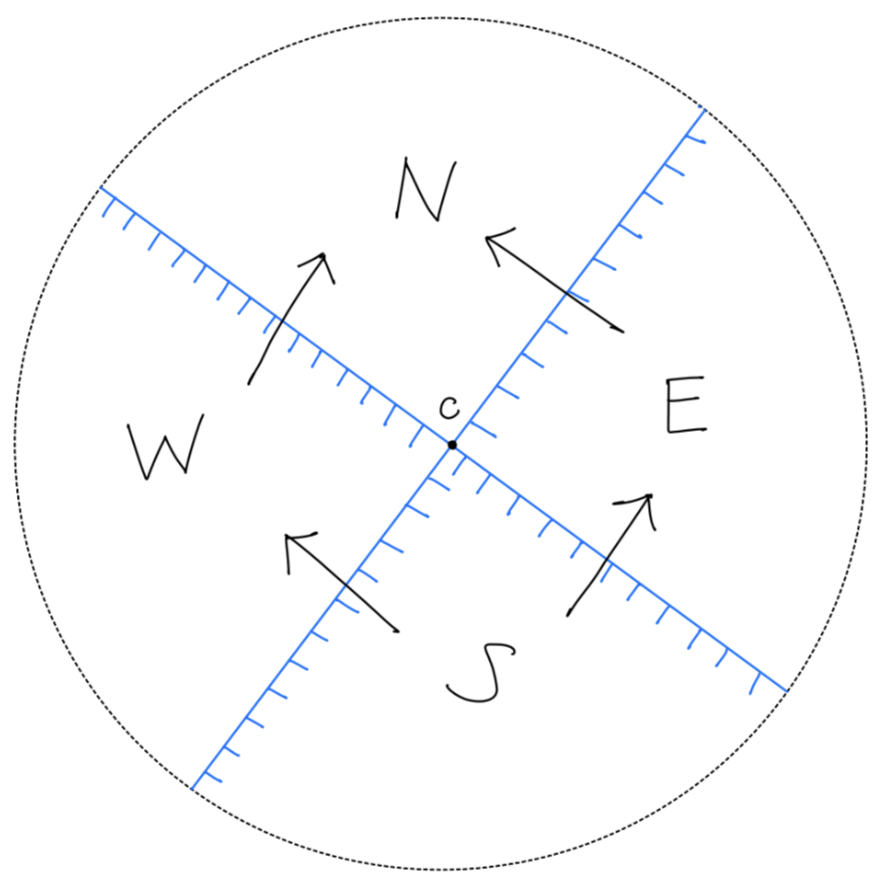
\includegraphics[scale = 0.55]{diagrams/intro/2.png}
    \caption{}
    \label{fig:your-label}
\end{figure}
then the total complex of 
\[
F^\bullet(S) \rightarrow F^\bullet(W)\oplus F^\bullet(E) \rightarrow F^\bullet(N)
\]
is acyclic.
\end{itemize}
\end{definition}
Suppose we have $\mathcal{S}$ a refinement of the stratification induced by $\Phi$ and a squiggly legible diagram $F^\bullet$, then we can make an object $\overline{F}^\bullet \in Fun^\bullet_\Lambda(\mathcal{S},\C)$ out of it in the following way.
\begin{definition}
$\rho : \mathcal{S} \rightarrow \{R\in \mathcal{S} \mid dim_\R(R) =2\}$ is a function that assigns $s\in \mathcal{S}$ to the smallest element in $\{R\in Vert(Q) \mid s \subset \overline{R}\}$.
\end{definition}

\begin{definition}
Suppose $F^\bullet$ is a squiggly legible diagram on $\mathcal{S}$, then we define $\overline{F}^\bullet \in Fun^\bullet _\Lambda (\mathcal{S},\C)$ where 
\begin{itemize}
\item for $s\in \mathcal{S}$, $\overline{F}^\bullet(s) := F^\bullet(\rho(s))$

\item for $s_1,s_2 \in \mathcal{S}$ such that $s_2 \subset star(s_1)$, $\overline{F}^\bullet (s_1 \rightarrow s_2) := F^\bullet(a_k)\circ \cdots F^\bullet(a_1)$ where $(a_1,a_2,\cdots,a_k)$ is a path from $\rho(s_1)$ to $\rho(s_2)$ in the quiver associated to $\mathcal{S}$. This is well-defined because the composition of cochain maps are path independent by the definition of squiggly legible diagram and the existence of a path from $\rho(s_1)$ to $\rho(s_2)$ is guaranteed by the fact that $Q_{s_2}$ is a subquiver of $Q_{s_1}$ and $\rho(s_2),\rho(s_1)$ are the smallest elements from each of them.
\end{itemize}
\end{definition}
In this paper, we only consider $\Phi$, $\Lambda$, and $\mathcal{S}$ that objects of $Fun^\bullet(\mathcal{S},\C)$ arises from squiggly legible diagrams.A variant of \cite[Prop~3.22.]{shende2017legendrian} shows that every objects of $Sh^\bullet_\Lambda(M;\C)$ is quasi-isomorphic to a squiggly legible diagram.

\subsection*{Microlocal Monodromy and Rank $1$ Objects}
In this section, we review the notion of microlocal monodromy of sheaves following\cite[Section~5.1]{shende2017legendrian}. For more general treatment, see \cite[Ch.~\MakeUppercase{\Rn{4}}]{kashiwara2013sheaves}. Supppose on $M$ we have a front diagram $\Phi$ and a stratification $\mathcal{S}$ that refines the one induced by $\Phi$ by adding squiggly line segments. Suppose we are given a sheaf $F^\bullet$ in terms of squiggly legible diagram, we define the associated sheaf on $\Lambda$, called microlocal monodromy denoted $\mu mon (F^\bullet)$, by assigning cochain complexes of $\C$-vector spaces for each one dimensional stratum contained in $\Phi$ and cochain maps between them for each point stratum contained in $\Phi$ as follows:
\begin{itemize}
\item if $s$ is a one dimensional stratum contained in $\Phi$, $\mu mon (F^\bullet)(s):=Cone(F^\bullet(s))$

\item if $p$ is a point stratum in $\Phi$, then $p$ is either a crossing or the endpoint of a squiggly line. We define the cochain map for each case as follows:
\begin{itemize}
\item when $p$ is a crossing, locally near $p$ the diagram looks like
\begin{figure}[H] 
    \centering
    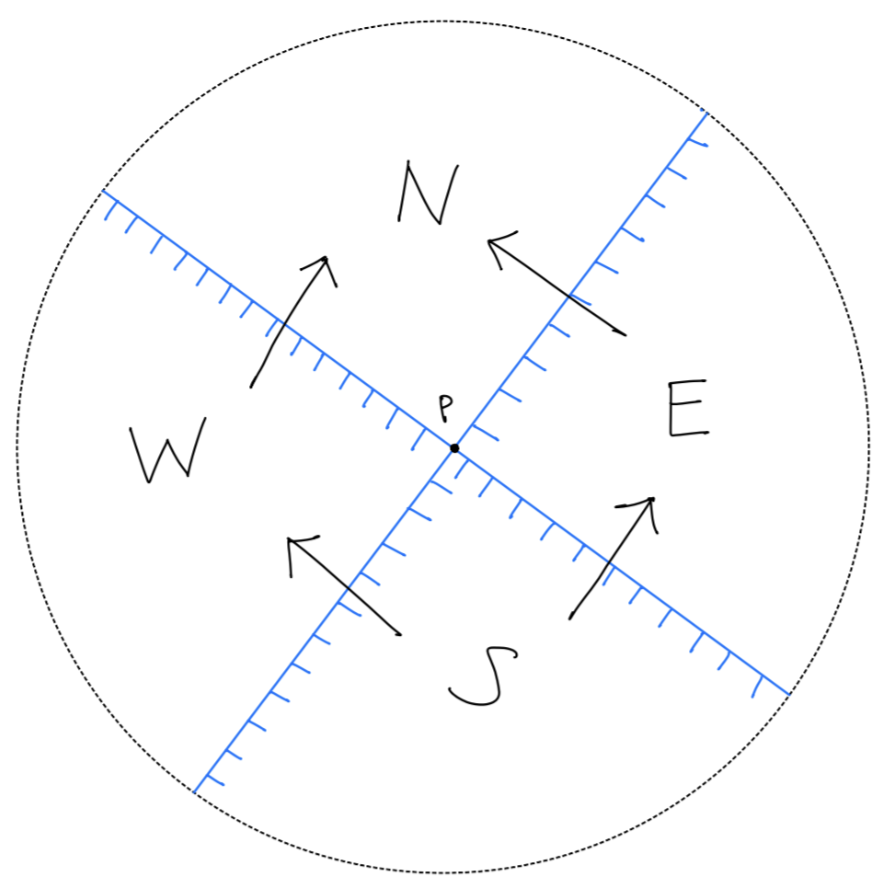
\includegraphics[scale = 0.55]{diagrams/intro/3.png}
    \caption{}
    \label{fig:your-label}
\end{figure}
then $p$ induces maps
\begin{align*}
& Cone(S\rightarrow W) \rightarrow Cone(E\rightarrow W)\\
& Cone(S\rightarrow E) \rightarrow Cone(W\rightarrow N)\\
\end{align*}

\item when $p$ is the endpoint of a squiggly line segment, locally near $p$ the diagram looks like one of the following diagrams 
\begin{figure}[H] 
    \centering
    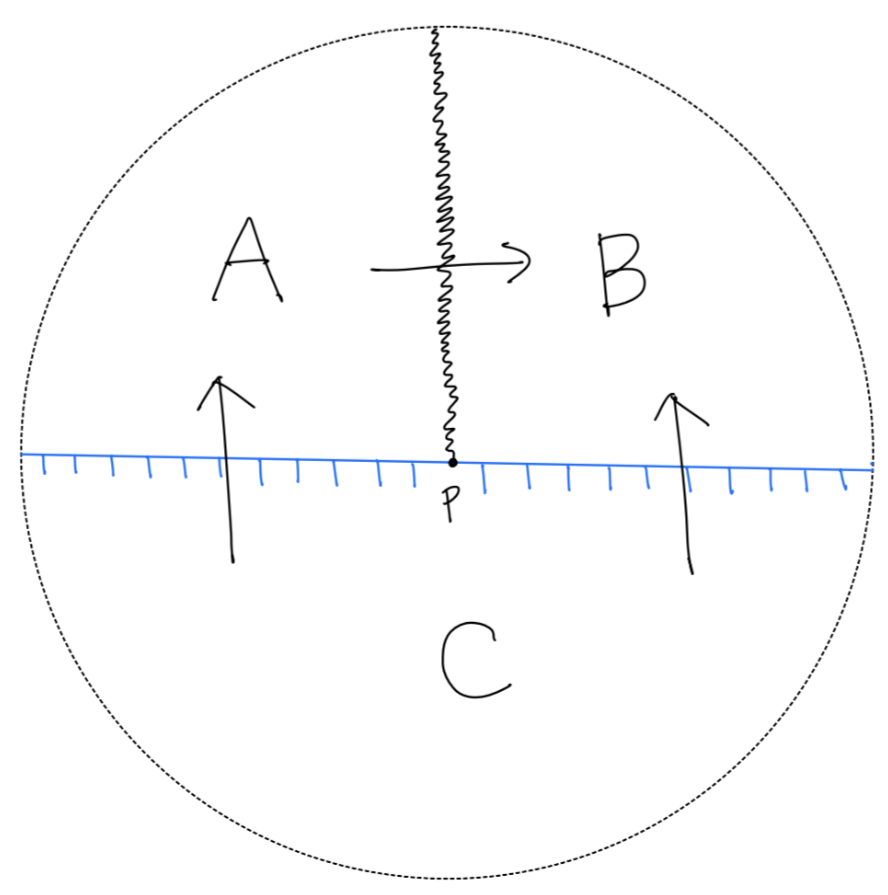
\includegraphics[scale = 0.55]{diagrams/intro/4.png}
    \caption{}
    \label{fig:your-label}
\end{figure}
\begin{figure}[H] 
    \centering
    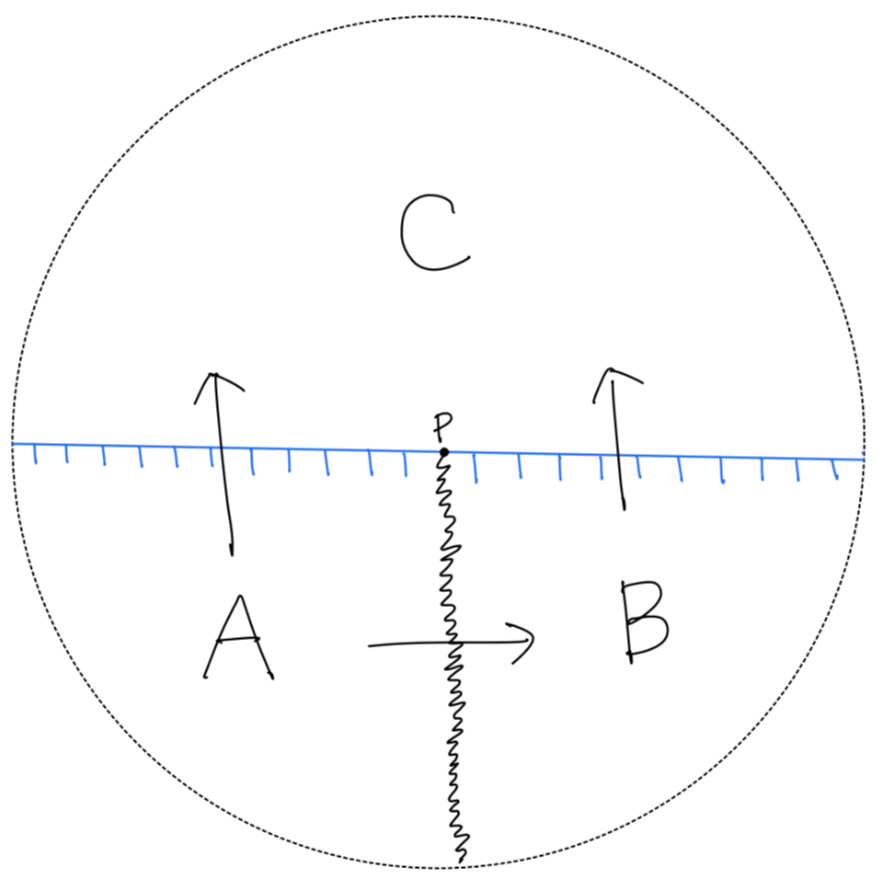
\includegraphics[scale = 0.55]{diagrams/intro/5.png}
    \caption{}
    \label{fig:your-label}
\end{figure}
\begin{figure}[H] 
    \centering
    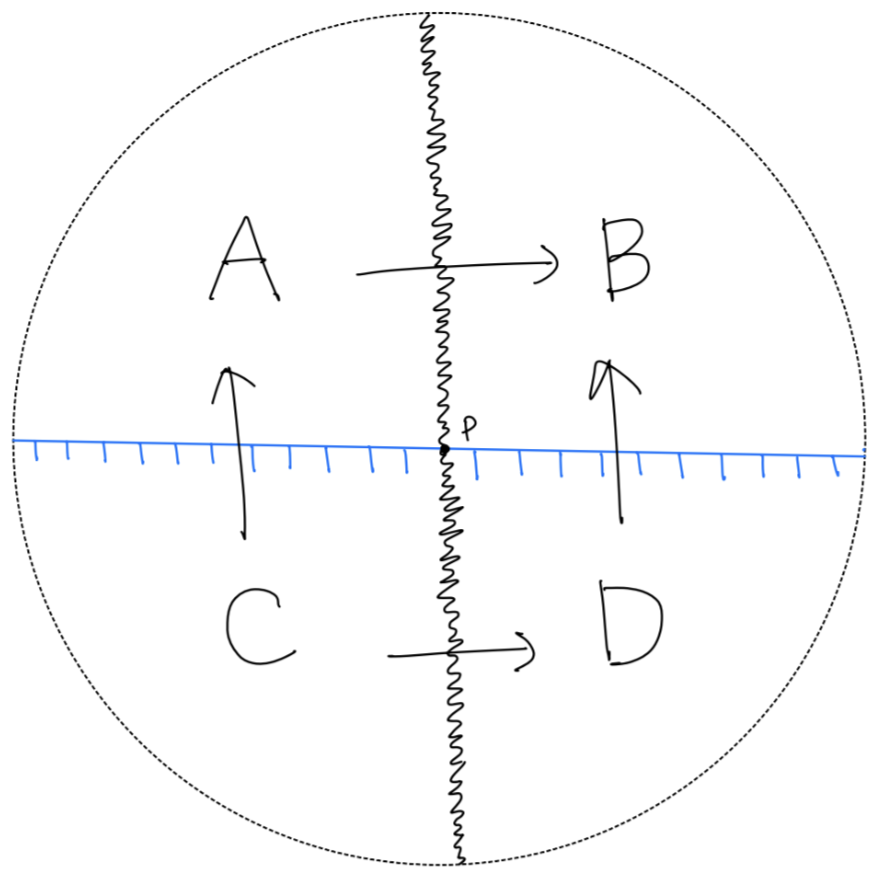
\includegraphics[scale = 0.55]{diagrams/intro/6.png}
    \caption{}
    \label{fig:your-label}
\end{figure}
, then we have a map
\begin{align*}
& Cone(C\rightarrow A) \rightarrow Cone(C\rightarrow B)\\
& Cone(A\rightarrow C) \rightarrow Cone(B\rightarrow C)\\
& Cone(C\rightarrow A) \rightarrow Cone(D\rightarrow B)\\
\end{align*}
respectively.
\end{itemize}
\end{itemize}
The maps between cones are quasi-isomorphisms because of the crossing condition and the fact that the map corresponding to squiggly lines are quasi-isomorphism.

\begin{definition}
$F^\bullet$ is called \emph{rank $n$ object} if $\mu mon (F^\bullet)$ is a rank $n$ local system concentrated in degree $0$ on $\Lambda$.
\end{definition}

\begin{definition}
The full subcategory of $Sh^\bullet_\Lambda(M;\C)$ containing rank $n$ objects is denoted $\mathcal{C}_n(M,\Lambda;\C)$ and the moduli stack classifying such objects $\mathcal{M}_n(M,\Lambda;\C)$. Additionally, let $\{\sigma_1,\cdots,\sigma_k\}$ be points in $M$ that are contained in one of the regions separated by $\Phi$. Then we define $\mathcal{C}_n(M,\Lambda, \{\sigma_1,\cdots,\sigma_k\};\C)$ to be the full subcategory of sheaves with vanishing stalks at $\{\sigma_1,\cdots,\sigma_k\}$, $\mathcal{M}(M,\Lambda, \{\sigma_1,\cdots,\sigma_k\};\C)$ the moduli space classifying such objects.
\end{definition}

\subsection*{Moduli Spaces associated to Positive Braids}
In this section, we define the moduli spaces associated to positive braids following\cite[Section~3]{shende2019cluster}. For background we refer to the survey \cite{toen2014derived} and the foundational works \cite{lurie2004derived} \cite{toen2009higher} \cite{toen2004hag} \cite{toen2005homotopical} \cite{toen2008homotopical}. Suppose we have a positive braid word $\omega$ of $n$ strands(i.e. a word freely generated by $s_1,\cdots,s_{n-1}$), Then we can think of its cylindrical closure in $S^1_\theta \times (0,1)_r = (\R_\theta /\Z) \times (0,1)_r$. In this paper, we consider two kinds of moduli spaces associated to the braid which are the main objects of study in Chapter2 and Chapter3 respectively.
\begin{enumerate}[label = (\arabic*)]
\item First, we embedd the cylinder containing cylindrical closure of $\omega$ in $M = S^1_x \times \R_z$ via $(\theta, r)\mapsto (\theta, r-1)$. We can think of the cylindrical closure of $\omega$ in $S^1_x \times \R_z$ co-oriented downward($z<0$) to be the front projection of a Legendrian knot $\Lambda_\omega$ living in $T^{\infty}M$. Let $\sigma_{z\ll 0}$ be a point in the non-compact region where $z\ll 0$. In Chapter2, we consider the moduli space $\mathcal{M}_1(S^1_x\times \R_z, \Lambda_\omega,\{\sigma_{z\ll 0}\};\C)$.

\item Next, we embed the cylinder containing the cylindrical closure of $\omega$ in $M = S^1_x \times \R_z$ via $(\theta,r) \mapsto (\theta,1-r)$ and embed the cylinder containing the cylindrical closure of the trivial braid $\omega_\emptyset$ via $(\theta,r)\mapsto (\theta,r-1)$. We get an embedding of the cylindrical closure of $\omega \coprod \omega_\emptyset$ in $S^1_x \times \R_z$ where the embedding of the cylindrical closure of $\omega$ is co-oriented upward and the embedding of the cylindrical closure of $\omega_\emptyset$ is co-oriented downward. We will call the embedding the separated diagram of $\omega$ and $\omega_\emptyset$ which we consider as the front projection of a Legendrian link $\Lambda_{\infty} \coprod \Lambda_{0} \subset T^{\infty}M$. Let $\sigma_{z\ll 0},\sigma_{z\gg 0}$ be points in the non-compact regions where $z\ll 0$ and $z\gg 0$. In Chapter3, we consider the moduli space $\mathcal{M}_1(S^1_x\times \R_z, \Lambda_\omega \coprod \Lambda_{\omega_\emptyset},\{\sigma_{z\ll 0}, \sigma_{z\gg 0}\};\C)$.
\end{enumerate}

\subsection*{Legendrian Isotopy and Sheaf Cobordism}
Invariance of the category $\mathcal{C}_1(M,\Lambda, \{\sigma_1,\cdots,\sigma_k\};\C)$ under Legendrian isotopy follows from the main theorem of \cite{guillermou2012sheaf}.
\begin{theorem}\label{GKS}
\cite{guillermou2012sheaf}. Suppose $\Lambda_0 \subset T^{\infty}M$ is a Legendrian and $\Lambda_\bullet \subset T^{\infty} \times [0,1]$ a Legendrian isotopy where $\Lambda_\bullet|_{T^{\infty} \times \{0\}}$ is equal to $\Lambda_0$ under the natural identification $T^{\infty} \times \{0\} \cong T^{\infty}$, then the restriction functor 
\[
Sh^\bullet_{\Lambda_\bullet}(M\times [0,1];\C) \rightarrow Sh^\bullet_{\Lambda_0}(M;\C)
\]
is a quasi-equivalence. Furthermore, this quasi-equivalence preserves rank $n$ objects.
\end{theorem}

\begin{definition}
Suppose we have a Legendrian isotopy $\Lambda_\bullet\subset T^{\infty} \times [0,1]$ from $\Lambda_0 = \Lambda_\bullet|_{T^{\infty} \times \{0\}}$ to $\Lambda_1 = \Lambda_\bullet|_{T^{\infty} \times \{1\}}$ and a sheaf $\mathscr{F}_\bullet \in Sh^\bullet_{\Lambda_\bullet}(M\times [0,1];\C)$ that restricts to $\mathscr{F}_0$ and $\mathscr{F}_1$ at $M\times\{0\}$ and $M\times\{1\}$, then we say $\mathscr{F}_\bullet$ is a \emph{sheaf cobordism} from $\mathscr{F}_0$ to $\mathscr{F}_1$.
\end{definition}

\begin{definition}
Suppose $\Lambda_0,\Lambda_1 \subset T^{\infty}M$ are Legendrian links and there is a Legendrian isotopy $\Lambda_\bullet \subset T^{\infty,-}M \times [0,1]$ where $\Lambda_\bullet|_{T^{\infty,-}\times \{0\}}$ is equal to $\Lambda_0$ under the natural identification $T^{\infty,-}\times \{0\} \cong T^{\infty,-}$ and $\Lambda_\bullet|_{T^{\infty,-}\times \{1\}}$ is equal to $\Lambda_0$ under the natural identification $T^{\infty,-}\times \{1\} \cong T^{\infty,-}$, then we have quasi- equivalence 
\[
Sh^\bullet_{\Lambda_0}(M;\C) \xrightarrow{\sim} Sh^\bullet_{\Lambda_1}(M;\C)
\]
from the following correspondence
\[
Sh^\bullet_{\Lambda_0}(M;\C) \xleftarrow{\sim} Sh^\bullet_{\Lambda_\bullet}(M\times [0,1];\C) \xrightarrow{\sim} Sh^\bullet_{\Lambda_1}(M;\C)
\]
Furthermore, this quasi-equivalence restricts to 
\[
\mathcal{C}_n(M,\Lambda_0;\C) \xrightarrow{\sim} \mathcal{C}(M,\Lambda_1;\C)
\]
When we have points $\{\sigma_1,\cdots,\sigma_k\}\subset M$ that are disjoint from the front projections of the Legendrian isotopy $\Lambda_\bullet$, we can further restrict the quasi-equivalence to
\[
\mathcal{C}_n(M,\Lambda_0,\{\sigma_1,\cdots,\sigma_k\};\C) \xrightarrow{\sim} \mathcal{C}_n(M,\Lambda_1,\{\sigma_1,\cdots,\sigma_k\};\C)
\]
\end{definition}

\subsection*{Alternating Legendrians}
\begin{definition}
Let $M$ be a surface and $\Lambda \subset T^{\infty}M$ a Legendrian link. An \emph{alternating coloring} for $\Lambda$ is the datum of, for each region in the complement of the front diagram, a label of black, white, or null, subject to the following conditions
\begin{itemize}
\item the boundary of a black region is co-oriented inward.
\item the boundary of a white region is co-oriented outward.
\item the boundary of the null region have both inward and outward co-orientations.
\item no black region shares a one dimensional border with white region and no null region shares a one dimensional border with another null region.
\end{itemize}
An \emph{alternating Legendrian} is a Legendrian equipped with an alternating coloring and their front projection is called an \emph{alternating strand diagram}. The \emph{bipartite graph} of the alternating Legendrian is the graph whose vertices are black and white regions. Edges are connected if their closure intersect and are of distinct color.
\end{definition}
Let $\hat{M}$ denote the real blow up of $M$ at the crossings of the front projection of $\Lambda$. The blow down map $\hat{M}\rightarrow M$ is a diffeomorphism away from the crossing and the fiber above a crossing is the $\R \mathbb{P}^1$ of lines tangent to the crossing. We define $W\subset M$($B\subset M$ resp.) the union of the interiors of the white(black resp.) regions of the complement of the front projection.

\begin{definition}
$\overline{L}$ denote the closure of the preimage of $W\cup B$ in $\hat{M}$. It is a smooth surface with boundary and we refer to its interior $L$ as the \emph{conjuate surface} of $\Lambda$.
\end{definition}

\begin{definition}\label{altsh}
An \emph{alternating sheaf} is an object of $Sh^\bullet_\Lambda(M;\C)$ whose support is contained in the closure of the union of the white and black regions.
\end{definition}

\begin{theorem}
\cite[Thm.~4.16]{shende2019cluster}\cite[Cor.~4.17]{shende2019cluster}. The full subcategory of $Sh^\bullet_\Lambda(M;\C)$ consisting of alternating sheaves is equivalent to the category of locally constant sheaves on $L$. Under this correspondence, rank $1$ local systems of corresponds to rank $1$ alternating sheaves.
\end{theorem}

\subsection*{Cluster Coordinates}
In this section, we review a special type of coordinate system on the moduli space $\mathcal{M}_1(S^1_x\times \R_z,\Lambda_\omega \coprod \Lambda_{\omega_\emptyset},\{\sigma_{z\ll 0},\sigma_{z\gg 0}\};\C)$ called cluster coordinate.\\
Suppose we have an alternating Legendrian $\Lambda_{alt}$ that is Legendrian isotopic to $\Lambda_{\omega}\coprod \Lambda_{\omega_\emptyset}$ via a Legendrian isotopy $\Lambda_{\bullet}$ whose front projection does not touch $\{\sigma_{z\ll 0},\sigma_{z\gg 0}\}$. Then the isotopy, by Theorem \ref{GKS}, induces an isomorphism between moduli spaces
\[
\mathcal{M}_1(S^1_x\times \R_z,\Lambda_{alt},\{\sigma_{z\ll 0},\sigma_{z\gg 0}\};\C) \xrightarrow{\sim}\mathcal{M}_1(S^1_x\times \R_z,\Lambda_\omega \coprod \Lambda_{\omega_\emptyset},\{\sigma_{z\ll 0},\sigma_{z\gg 0}\};\C)
\]
Furthermore, once we have alternating Legendrian, we can construct its conjugate surface $L$ which deformation retracts to the bipartite graph $\Gamma_{\Lambda_{alt}}$ of alternating coloring on $\Lambda_{alt}$. Therefore, there is a sequence of isomorphisms
\[
H^1(L,\C^*) \cong H^1(\Gamma_{\Lambda_{alt}},\C^*) \cong (\C^*)^{b_1(\Gamma_{\Lambda_{alt}})}
\]
where $b_1(\Gamma_{\Lambda_{alt}})$ is the $1^{st}$ Betti number of $\Gamma_{\Lambda_{alt}}$.\\
Also, local systems on $L$ corresponds to alternating sheaves in $M_1(S^1_x\times \R_z, \Lambda_{alt},\{\sigma_{z<<0},\sigma_{z>>0}\};\C)$ i.e. we have an inclusion
\[
H^1(L,\C^*)\hookrightarrow M_1(S^1_x\times \R_z, \Lambda_{alt},\{\sigma_{z<<0},\sigma_{z>>0}\};\C)
\]
In conclusion, we have an inclusion
\[
(\C^*)^{b_1(\Gamma_{\Lambda_{alt}})}\hookrightarrow M_1(S^1_x\times \R_z, \Lambda_{\omega}\coprod \Lambda_{\omega_{\emptyset}},\{\sigma_{z<<0},\sigma_{z>>0}\};\C)
\]
which is called a \emph{cluster coordinate chart} of the moduli space. There is a rich theory of ``cluster varieties", covered by such cluster coordinate charts, but in this thesis we only construct one such chart.\\
\section{Summary of results}\label{sec_summary_of_results}

\subsubsection*{Chapter 2}

We define a class of braid words that we call \emph{Sibuya braid words}. We show that the moduli spaces $\mathcal{M}_1(S^1_x \times \R_z, \Lambda_\omega, \{\sigma_{z\ll 0}\};\C)$ associated to Sibuya braid words $\omega$ parametrize configurations of points on a Projective space subject to certain non-degeneracy conditions. They are a generalization of the Sibuya space that Boalch studied in \cite{sibuya1975global}\cite{boalch2015wild}. Their definition and a simple combinatorial characterization can be found in  Definition \ref{Sibuya} and Theorem \ref{combinatorial}. In this introduction, I will illustrate the concept with an example.\\ 
Consider a braid word $\omega =(s_1 s_2)^2$ on $3$ strands, which is a power of the Coxeter braid. Then we have an embedding of $\omega$ into the fundamental domain of $S^1_x\times \R_z$ given in the below figure
\begin{figure}[H] 
    \centering
    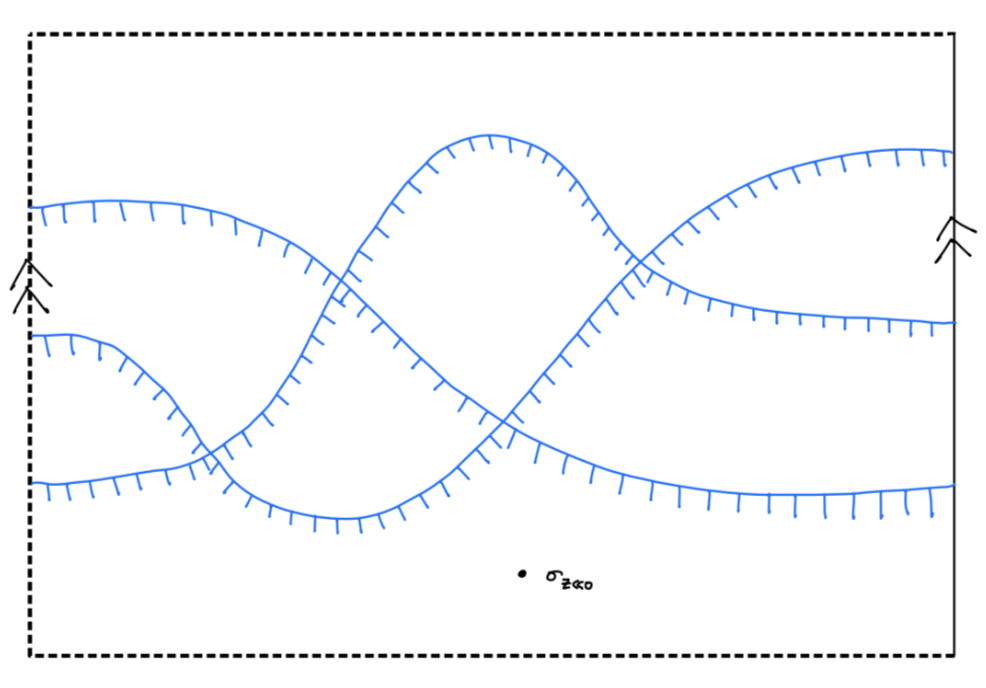
\includegraphics[scale = 0.55]{diagrams/intro/7.png}
    \caption{}
    \label{fig:your-label}
\end{figure}
Since the stratification induced by $\omega$ is not a regular cell complex, for example non-compact regions at the top and the bottom are not contractible, we refine it by adding squiggly lines co-oriented towards left.
\begin{figure}[H] 
    \centering
    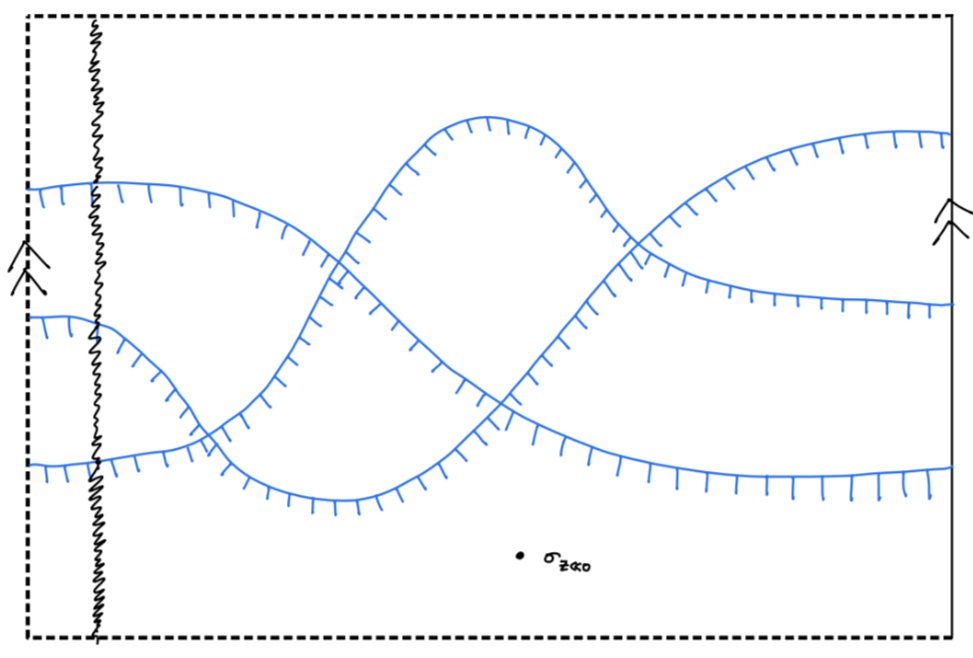
\includegraphics[scale = 0.55]{diagrams/intro/8.png}
    \caption{}
    \label{fig:your-label}
\end{figure}
Consider an object of $C_1(S^1_x \times \R_z, \Lambda_\omega, \{\sigma_{z\ll 0}\};\C)$. It can be described as a squiggly legible diagram by assigning cochain complexes of $\C$-vector spaces to regions and cochain maps to arcs subject to the conditions mentioned in (legible object subsection). Let's check how those conditions translates to our situation:
\begin{itemize}
\item the cochain complex assigned to the bottom region, which we call height $0$ region, is acyclic because of the vanishing condition at $\sigma_{z\ll 0}$. We are considering cochain complexes of sheaves upto quasi-isomorphism, so we assign $0$ stalk to the region.

\item the stalk at the regions adjacent to the height $0$ region that are not a height $0$ region, which we call height $1$ regions, should be quasi-isomorphic to dimension $1$ vector space $\C$ because of the microlocal rank $1$ condition on blue arcs separating height $0$ region and height $1$ regions i.e. the mapping cone of the cochain map corresponding to blue arcs should be rank $1$ vector spaces concentrated in degree $0$. Therefore, we assign $\C$ to these height $1$ regions and incoming maps from the height $0$ region zero maps.

\item the stalk at the regions adjacent to the height $1$ regions that are not height $0,1$ regions, which we call height $2$ regions, should be quasi-isomorphic to dimension $2$ vector space $\C^2$ and incoming maps from the height $1$ region to be monomorphisms because of the microlocal rank $1$ condition again. Therefore, we assign $\C^2$ to the height $2$ regions and incoming maps from the height $1$ regions to be inclusion maps.

\item Now, we are left with one non-compact region at the top which we call height $3$ region. Again by microlocal rank $1$ condition, the stalk should be $\C^3$ and the incoming maps from height $2$ regions are inclusion maps.

\item the maps corresponding to squiggly lines are isomorphisms of adjacent vector spaces.

\item all diagrams should commute.

\item for each crossing the crossing condition translates to
\begin{figure}[H] 
    \centering
    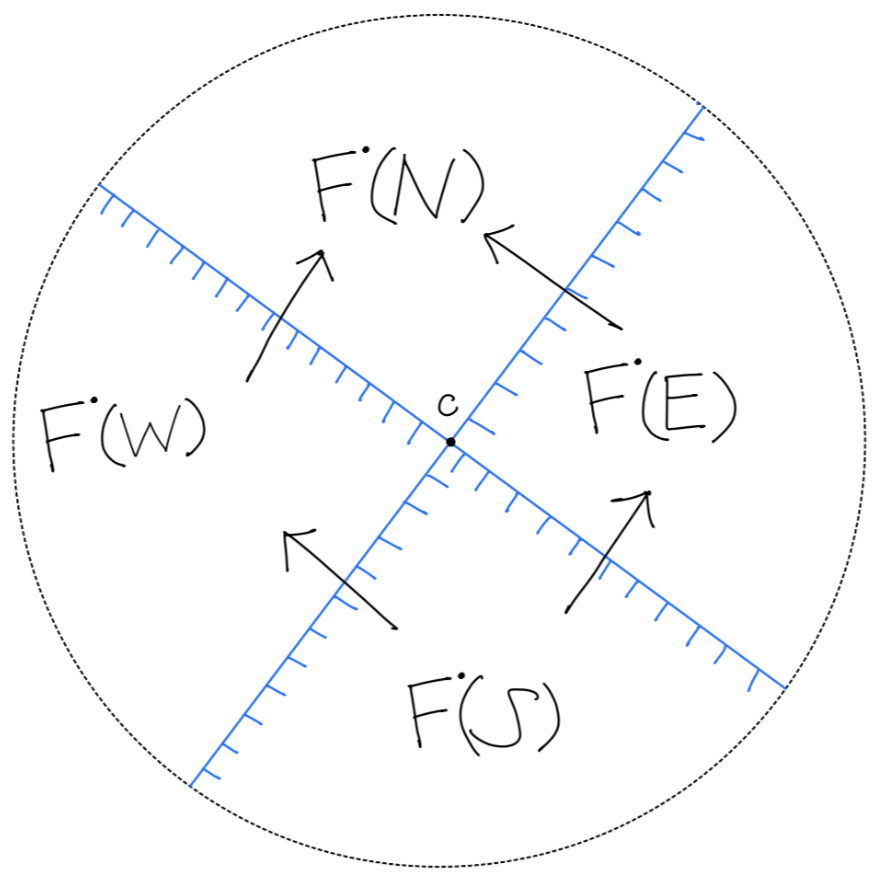
\includegraphics[scale = 0.55]{diagrams/intro/9.png}
    \caption{}
    \label{fig:your-label}
\end{figure}
\begin{figure}[H] 
    \centering
    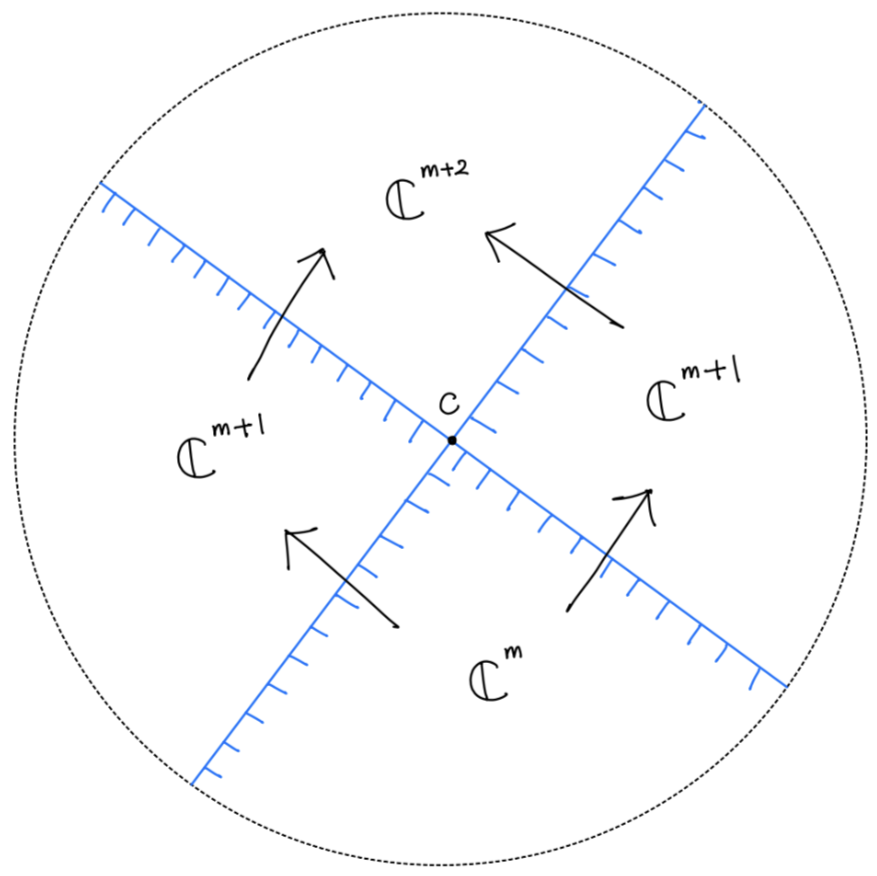
\includegraphics[scale = 0.55]{diagrams/intro/10.png}
    \caption{}
    \label{fig:your-label}
\end{figure}
the inclusion of $F^\bullet(W)$ and $F^\bullet(E)$ in $F^\bullet(N)$ intersects transversely in $F^\bullet(S)$.
\end{itemize}

In summary, an object of $C_1(S^1_x\times \R_z,\Lambda,\{\sigma_{z\ll 0}\};\C)$ amounts to the data of assigning 
\begin{itemize}
\item  dimension $i$ subspaces of $\C^3$ to height $i$ regions subject to the condition that $F^\bullet(W)+F^\bullet(E) = F^\bullet(N)$ and $F^\bullet(W)\cap F^\bullet(E) = F^\bullet(S)$.

\item an element $g \in GL_3(\C)$ that maps the subspaces corresponding to the region to the left of squiggly lines to the subspaces corresponding to the region to the right of the squiggly lines.
\end{itemize}
One thing to note in the above example is that once we assign the dimension $1$ subspaces to the height $1$ regions, all the other subspaces are determined by the crossing conditions. More precisely, we can construct subspaces that are assigned to the regions of heights greater than $1$ as follows: Suppose $R$ is a region, then the subspace we assign to $R$ is the subspace of $\C^3$ spanned by the $1$ dimensional subspaces assigned to the height $1$ regions that have paths to $R$. I will describe what this means in Chapter2. This fact that the sheaf is completely determined by its rank $1$ stalks relies on following feature of the diagram $\Lambda_\omega$:
\begin{quote}
Every region of height bigger than $1$ has more than or equal to $2$ different regions of height $1$ less adjacent to it.
\end{quote}
We call a braid word with the above property as Sibuya braid word and a braid with Sibuya braid word representation as Sibuya braid.\\
But also note that not all assignments of $1$ dimensional subspaces of $\C^3$ to height $1$ regions gives rise to legitimate sheaves. In Chapter2, I will show how to restate the crossing conditions using only rank $1$ stalks.\\
At the end of the Chapter, we will explicitly compute examples of the generalized Sibuya space.
\subsubsection*{Chapter 3}
Chapter3 is the longest chapter in the thesis, but we can summarize it more briefly:
\begin{enumerate}[label = (\roman*)]
\item we will systematically construct a natural alternating Legendrian(equivalently, alternating strand diagram) that are Legendrian isotopic to the separated Legendrian $\Lambda_\omega \coprod \Lambda_{\omega_\emptyset} \subset T^\infty(S^1_x \times \R_z)$.

\item we will construct a Legendrian isotopy between the alternating Legendrians and the separated Legendrians.

\item we will explicitly describe the sheaf cobordism induced by the above isotopy.
\end{enumerate}


\section*{Conventions and notation}\label{sec_conventions}
\begin{itemize}[label={--}]
\item $\omega$ denotes positive braid words. In this thesis, all braid words are positive braid words.

\item $\beta$ denotes positive braids. In this thesis, all braids are positive braids.

\item $\operatorname{Cross}(\omega)$ denotes the set of crossings in the braid word $\omega$.

\item $L$ denotes Lagrangian surfaces in $T^*(S^1_x\times \mathbb{R}_z)$.

\item $\Lambda,\lambda$ denote Legendrian links in $T^\infty(S^1_x\times \mathbb{R}_z)$.

\item $\Xi,\xi$ denote co-orientations on Legendrian links.

\item $\Phi$ denotes front projections of Legendrian links on $S^1_x \times \mathbb{R}_z$.

\item $\mathcal{S}$ denotes refinements of the stratifications induced by front projections.

\item $\mathscr{F}^\bullet$ denotes a cochain complex of sheaves whose cohomologies are constructible sheaves. We simply call these ``sheaves" in this thesis.

\item $Q$ denotes quivers.

\item $\operatorname{Vert}(Q)$ denotes the set of vertices of the quiver $Q$.

\item $\operatorname{Arr}(Q)$ denotes the set of arrows of the quiver $Q$.

\item $\Upsilon^k_0$ denotes the set of signature $0$ height $k$ vertices in a quiver.

\item $I_k(v)$ denotes the set of height $1$ vertices that have paths to vertex $v$ in a quiver.

\item $\operatorname{SS}(\mathscr{F}^\bullet)$ denotes the singular support of the sheaf $\mathscr{F}^\bullet$.

\item $\mu mon(\mathscr{F}^\bullet)$ denotes the microlocal monodromy sheaf of $\mathscr{F}^\bullet$.

\item $Sh^\bullet(M;\mathbb{C})$ denotes the dg category of sheaves on $M$.

\item $Sh^\bullet_L(M;\mathbb{C})$ denotes the full subcategory of $Sh^\bullet(M;\mathbb{C})$ whose singular support is contained in the Lagrangian $L$.

\item $Sh^\bullet_\Lambda(M;\mathbb{C})$ denotes the full subcategory of $Sh^\bullet(M;\mathbb{C})$ whose singular support is contained in the Lagrangian $\mathbb{R}_+ \Lambda \cup 0_M$.

\item $Fun^\bullet(\mathcal{S},\mathbb{C})$ denotes the dg category of functors from the poset category $\mathcal{S}$ to the category of cochain complexes of $\mathbb{C}$-vector spaces.

\item $Fun^\bullet_\Lambda(\mathcal{S},\mathbb{C})$ denotes the full subcategory of $Fun^\bullet(\mathcal{S},\mathbb{C})$ whose objects under the quasi-equivalence $\Gamma_\mathcal{S}$ (see \ref{KS}) correspond to sheaves singular supported in $\mathbb{R}_+ \Lambda \cup 0_M$.

\item $F^\bullet$ denotes quiver representations valued in the cochain complex of $\mathbb{C}$-vector spaces.

\item $\overline{F}^\bullet$ denotes objects of $Fun^\bullet(\mathcal{S},\mathbb{C})$.

\item $\mathcal{C}_n(M,\Lambda,\{\sigma_1,\cdots,\sigma_k\};\mathbb{C})$ denotes the full subcategory of $Sh^\bullet_\Lambda(M;\mathbb{C})$ consisting of rank $n$ objects.

\item $\mathcal{M}_n(M,\Lambda,\{\sigma_1,\cdots,\sigma_k\};\mathbb{C})$ denotes the moduli space parametrizing objects of $\mathcal{C}_n(M,\Lambda,\{\sigma_1,\cdots,\sigma_k\};\mathbb{C})$.

\item $\mathcal{M}_\omega$ denotes the moduli space $\mathcal{M}_1(S^1_x \times \mathbb{R}_z,\Lambda_\omega,\{\sigma_{z\ll 0}\};\mathbb{C})$.

\item $\mathcal{M}_\omega^{fr}$ denotes the framed moduli space of $\mathcal{M}_\omega$, i.e., the moduli space parametrizing the objects of $\mathcal{M}_\omega$ with a choice of basis for the stalk at $\sigma_{z\gg 0}$, a fixed point in the non-compact region $z\gg 0$.

\item $\iota_\omega$ denotes the embedding of $\mathcal{M}_\omega^{fr}$ in the product of a general linear group with powers of projective spaces, i.e., $GL_n(\mathbb{C}) \times (\mathbb{P}^{n-1})^k$.

\item $L_{conj}$ denotes the conjugate surface of an alternating Legendrian.

\item $\Gamma_{bi}$ denotes the bipartite graph associated to an alternating Legendrian.

\item $\Psi(x_0,r_0,z_{lo},z_{hi})$ denotes the bump function about $x=x_0$ of radius $r_0$, with $z$ range from $z_{lo}$ to $z_{hi}$ i.e. consider the standard bump function 
$$\Psi_0(x) = \begin{cases}
  e^{\frac{1}{x^2 -1}}, & |x| < 1 \\
  0, & |x| \geq 1
  \end{cases}$$
then
\[
\Psi(x_0,r_0,z_{lo},z_{hi}) := (z_{hi} - z_{lo})\Psi(\frac{x-x_0}{r_0}) + z_{lo}
\]
We denote the bump function about $x=0$ of radius $1$ by $\Psi(z_{lo},z_{hi})$.

\item $\tau$ denotes the smooth transition function i.e. consider the function
  $$f(x) = \begin{cases}
  e^{-\frac{1}{x}}, & x > 0 \\
  0, & x \leq 0
  \end{cases}$$
then
  $$\tau(x) = \frac{f(x)}{f(x)+f(1-x)}$$

\item $I$ denotes an identity matrix. We omit the size of the matrix when it can be inferred from context.

\item $I_{i_0,j_0}$ denotes the matrix whose $(i,j)$-entry is $\delta_{i,i_0}\cdot \delta_{j,j_0}$ where $\delta$ is the Kronecker delta.

\item Let $T$ be an $n$ by $m$ matrix, then $T(r_{start},r_{end},c_{start},c_{end})$ denotes the truncation of the matrix $T$ with row range from $r_{start}$ to $r_{end}$ and column range from $c_{start}$ to $c_{end}$.

\item $\text{diag}(a_1,\cdots, a_k)$ denotes the diagonal matrix of size $k\times k$ whose $(i,i)$-entry is $a_i$.

\item $e_i$ denotes the $i^{\text{th}}$ standard basis vector of $\mathbb{C}^m$.

\item $\iota_k$ denotes the monomorphism from $\mathbb{C}^m$ to $\mathbb{C}^{m+1}$ that maps $e_i$ to $e_{i+k}$. We omit the dimensions of the source and the target vectorspaces when it can be inferred from the context.

\item $D_{r=r_0}$ denotes the standard disk in $\mathbb{R}^2$ of radius $r_0$ centered at the origin.

\item Let $(C^\bullet,\delta^\bullet)$ and $(C'^\bullet,\delta'^\bullet)$ be cochain complexes supported in degrees $0$ and $1$, and let $\phi^\bullet$ be a morphism between $(C^\bullet,\delta^\bullet)$ and $(C'^\bullet,\delta'^\bullet)$. Then:
\begin{itemize}[label = $\circ$]
\item We denote $(C^\bullet,\delta^\bullet)$ as either:
\begin{itemize}
\item $C^0 \xrightarrow{\delta^1} C^1$
    
    or
    
\item $\begin{array}{c}
      C^1 \\
      \uparrow^{\delta^1} \\
      C^0
      \end{array}$
\end{itemize}
\item We denote $\phi^\bullet$ as either:
\begin{itemize}
\item ($\phi^0$, $\phi^1$)
    
    or
    
\item $\begin{array}{ccc}
      C^1 & \xrightarrow{\phi^1} & C'^1 \\
      \uparrow^{\delta^1} & & \uparrow^{\delta'^1} \\
      C^0 & \xrightarrow{\phi^0} & C'^0
      \end{array}$
\end{itemize}
\item We omit coboundary maps ($\delta^1$) or cochain maps ($\phi^i$ for $i=0,1$) when either the source or the target is $0$, in which case the map is obviously a zero map.
    
\item When the source and target vector spaces of coboundary maps ($\delta^1$) or cochain maps ($\phi^i$ for $i=0,1$) are identical and the map between them is omitted, it is understood to be an identity map.

\end{itemize}
\item When drawing a squiggly legible diagram, we follow these conventions:
\begin{itemize}[label=$\circ$]
\item All maps corresponding to red arcs are $\iota_0$ unless otherwise specified.
  
\item All maps corresponding to blue arcs are $\iota_1$ unless otherwise specified.
  
\item Stalks and generization maps are omitted when they can be inferred from the context.
\end{itemize}
\end{itemize}

%%%%%%%%%%%%%%%%%%%%%%%%%%%%%%%%%%%%%%%%%%%%%%%%%%%%%%%%%%%%%%%%%%%%%%%%%%%%%%%%%%%%%%%%
%%%%%%%%%%%%%%%%%%%%%%%%%%%%%%%%%%%%%%%%%%%%%%%%%%%%%%%%%%%%%%%%%%%%%%%%%%%%%%%%%%%%%%%%

\chapter{Multivalent braids and wild character varieties of Sibuya type}
\section{Basic terminologies} 
\begin{definition}
	Let $\omega$ be a braid word representing a braid $\beta\in Br_n^+$ i.e. $[\omega] = \beta$. Then we define $Q_{\omega}$ to be the quiver 
\begin{itemize}
		\item whose vertices are labeled by the regions of the front projection(note that this front projection is defined on $\mathbb{R}^2$ not on a cylinder)
		\item whose arrows are labeled by pairs of vertices whose corresponding regions are adjacent(bordered by the front projection of the braid) subject to the condition that the arrows always go against the co-orientation(hairs).
	\end{itemize}
There are two distinguished vertices of $Q_\omega$. We denote the vertex corresponding to the region $z\rightarrow \infty$(resp. $z\rightarrow -\infty$) as $U$(resp. $D$).
\end{definition}
Maybe good to have an example after each definition.
\begin{definition}
	Locally for each crossing $c$, there is a region all the hairs are pointing outward, we call this $n_c$(read north of $c$). Starting from $n_c$, as we move counter-clockwise about the crossing, we call the corresponding regions $n_c,e_c,s_c,w_c$ respectively(read north of, east of, south of, west of $c$).
\end{definition}
\begin{theorem}
	Suppose we have a fixed braid word $\omega$ and $v$ is a vertex corresponding to a region given by the front projection of $\omega$. Any path from $d$ to a vertex $v$ have same length.
\end{theorem}
\begin{proof}
we prove the statement by the induction on the length of the braid words. The statement is trivial for trivial braid word because there is only one path from d to any vertex. Suppose the statement is true for all quivers associated to braid words whose length is less than $n$. Suppose $\omega$ is a braid word of length $n$. Suppose there are two distinct paths $p_1$ and $p_2$ from $d$ to $v$. Let $\omega = s_{i_1}\cdots s_{i_n}$. There are two cases to consider :\\
(case1) $v$ is the region east of the new crossing generated by $s_{i_n}$. Then the paths to $v$ must have passed the region right below the region of $v$ because that's the only possible way to get to $v$ under the constraint that the arrow always go against the co-orientation. If we remove the last edge and vertex from the paths $p_1,p_2$, we have paths $p'_1,p'_2$ ending at the same vertex(i.e. south of the crossing generated by $s_{i_n}$) and are entirely contained in the subquiver $Q_{\omega '}$ where $\omega ' = s_{i_1}\cdots s_{i_{n-1}}$. Therefore, by the induction hypothesis the lengths of $p'_1$ and $p'_2$ are the same which immediately implies $length(p_1) = length(p'_1) + 1 =length(p'_2) + 1 = length(p_2)$.\\
(case2) Suppose $v$ is not the region that is the east of the crossing generated by $s_{i_n}$. Without loss of generality, we can assume that two paths do not pass through the region east of the crossing, because we can always replace the part of the path $s_c\rightarrow e_c \rightarrow n_c$ with $s_c\rightarrow w_c \rightarrow n_c$ having the same length. Then once we know that two paths $p_1$ and $p_2$ do not pass through the region east of the crossing, we know that they are entirely contained in the subquiver $\omega ' = s_{i_1}\cdots s_{i_{n-1}}$. Then the $length(p_1) = length(p_2)$ by the induction hypothesis.
\end{proof}


\begin{definition}
 The valency of the vertex of a quiver is the number of incoming arrows. The height of the vertex of a quiver is the length of a path starting from $d$ ending at that vertex which is well-defined by the previous theorem. Note that for every crossing $c$, $e_c$ and $w_c$ have the same height. 
\end{definition}

\begin{definition}
 We say two vertices are adjacent if there is a crossing $c$ such that two vertices are $e_c$ and $w_c$ of this crossing. Let $k$ be a positive integer, then we define a natural ordering on the set of all height $k$ vertices generated by the following relations : For each crossing $w_c \leq e_c $.
 
\end{definition}

\begin{theorem}
	The above ordering is well-defined and is a total ordering on the set of all height $k$ vertices.
\end{theorem}

\begin{proof} 
To prove the claim, we have to prove the following facts :
\begin{enumerate}[label=(\roman*)]
	\item For any two distinct points of height $k$, there is a chain of crossings connecting two points.
	\item there is no chain of crossings starting at a point and ending at the same point.
\end{enumerate}
We prove the claim by induction on the length of braid words. For the trivial braid, (\Rn{1}) holds because there is only one vertex for each height and (\Rn{2}) holds because there is no arrow starting from that unique and ending at the point.\\
 Now suppose the claim holds for all $length < n$ braids and suppose $Rn{1}$ does not hold for the braid word $\omega = s_{i_1}\cdots s_{i_n}$. Then one of the two vertices should be the vertex corresponding to $e_c$ of the crossing generated by $s_{i_n}$. Let's call this vertex $v$ and the other as $v'$. Then we know that by the induction hypothesis there is a chain of crossing connecting $v'$ and $w_c$. Since $w_c$ is connected by the crossing $c$ to $e_c = v$ and $v$,$v'$ are connected by a chain of crossings which is a contradiction. \\
 Now suppose the claim holds for all $length < n$ braids and suppose $Rn{2}$. Suppose there is a point where there is a chain of crossing starting and ending at the same point. By the induction hypothesis, the chain of crossing generated by $s_{i_n}$ along the way. Without loss of generality, using cyclic shift we can assume the chain of crossings starts from $e_c$ which is a contradiction because $e_c$ is not the $w_c'$ of any crossing $c'$.
\end{proof}


\begin{definition}
	 There are two distinguished type $A$ sub-quivers of $Q_{\omega}$. We denote $R_{\omega}$(resp. $L_{\omega}$) to be the full sub-quiver containing all the vertices corresponding to the rightmost(resp. leftmost) regions. Alternatively, the path following the largest(resp. smallest) arrows at each step. We denote the vertex of $R_{\omega}$(resp. $L_{\omega}$) of height $k$ by $R^k_{\omega}$(resp. $L^k_{\omega}$).
\end{definition}

\begin{definition}
	Let $\mathcal{M}^{fr}_{\omega}$ be the framed moduli space classifying pairs $(F,g)$ where $F$ is the representation of $Q_{\omega}$ and $g\in GL_n(\mathbb{C})$ subject to the following conditions:
	\begin{itemize}
		\item For each vertex the vectorspace associated to it is a subspace of $\mathbb{C}^n$ of dimension equal to its height.
		\item  All maps are inclusion maps.
		\item  $gF(R^k_{\omega})=F(L^k_{\omega})$ for all $k=0,1,\cdots, n$.
		\item For each crossing $c$, then the sequence $0\rightarrow F(s_c)\rightarrow F(e_c)\oplus F(w_c)\rightarrow F(n_c)\rightarrow 0$ is a short exact sequence where maps are induced by the inclusion maps.
	\end{itemize}
\end{definition}

\begin{remark}
	There is a natural left action of $x\in GL_n(\mathbb{C})$ on $(F,g)\mathcal{M}^{fr}_{\omega}$, that is, $x\cdot(F,g)=(xF,xGx^{-1})$ where $xF$ is left translation on quiver representation and $xgx^{-1}$ is conjugation.
\end{remark}

\begin{theorem}
	$\mathcal{M}(\beta^{\circ})\cong GL_n(\mathbb{C})\backslash \mathcal{M}^{fr}_{\omega}$. By $\mathcal{M}(\beta^{\circ})$ I mean the moduli space defined in STZ.
\end{theorem}
\begin{proof} 
maybe in STZ or STWZ??
\end{proof}

Now consider the following map
\begin{definition}
Suppose we have the braid word $\omega$ of a braid $\beta$. Let $\{v_1,v_2,\cdots,v_m\}$ be the complete list of all height 1 vertices of $Q_{\omega}$ such that $v_i<v_j$ if and only if $i<j$. We define $\iota_\omega$ to be the  forgetful map 
\begin{align*}
\iota_{\omega}~:~ &\mathcal{M}^{fr}_{\omega}\rightarrow(\mathbb{P}^{n-1})^m\times GL_n(\mathbb{C})\\
& (F,g) \mapsto ([F(v_1)],\cdots,[F(v_m)], g)
\end{align*}
\end{definition}

\begin{definition}
	Let $\omega$ be a braid word. We denote the infinite cyclic copies of the original braid word $\omega$ by $\omega^\infty$. More precisely, suppose $\omega$ is a braid word given by a collection of sections $\{\sigma_i : [0,1]_x\rightarrow [0,1]_x\times \mathbb{R}^2_{y,z}\}_{i =1,\dots,n}$, then $\omega^\infty$ is given by the collection $\{\overline{\sigma_i} : \mathbb{R}_x\rightarrow \mathbb{R}^3_{x,y,z} ~|~ \overline{\sigma}(x,y,z) = \sigma(x-[x],y,z)\}_{i =1,\dots,n}$. Again, I will abuse the notation $\omega^\infty$ to denote its front projection onto $\mathbb{R}^2_{x,z}$. 
\end{definition}	
	
	
	
\begin{definition}	
	Let $\omega$ be a braid word, then we have the quiver $Q_\omega$ associated to it. We define the quiver $Q_\omega^\infty$ to be the quotient of  $\prod_{i \in \mathbb{Z}} Q_\omega$ by the relations $\{R_{\omega,i} = L_{\omega,i+1}\}_{i\in \mathbb{Z}}$ where $R_{\omega,i}$(resp. $L_{\omega,i+1}$) is the subquiver $R_{\omega}$(resp. $L_{\omega}$) in the $i^{th}$(resp. $i+1^{th}$) copy of $Q_\omega$ in $\prod_{i \in \mathbb{Z}} Q_\omega$. Therefore, we have the quotient map of quivers $q : \prod_{i \in \mathbb{Z}} Q_\omega \rightarrow Q_\omega^\infty$. Let the signature function $\sigma' : Vert(\prod_{i \in \mathbb{Z}} Q_\omega) \rightarrow \mathbb{Z}$ be $\sigma'(v) = i$ if $v$ is in the $i^{th}$ copy of $Q_\omega$ in $\prod_{i \in \mathbb{Z}} Q_\omega$. Define $\sigma : Q_\omega^\infty \rightarrow \mathbb{Z}$ to be $\sigma(v) = min_{w\in q^{-1}(v)} \sigma'(w)$ if $|q^{-1}(v)| < \infty$ and $0$ otherwise. Note that for $v\in Vert(Q_\omega^\infty)$, $q^{-1}(v)$ is infinite if and only if $R_\omega^{height(v)} = L_\omega^{height(v)}$ i.e. there is a unique vertex of $height(v)$ in $Q_\omega$. We can think of $Q_\omega$ as the full subquiver of $Q_\omega^\infty$ spanned by the signature $0$ vertices. 
\end{definition}

\begin{definition}	
Suppose we have a quiver representation $F_\omega$ of $Q_\omega$, then we define the induces quiver representation $F^{\infty}_{\omega}$ of the quiver $Q^{\infty}_{\omega}$ to be $F_\omega^\infty(v) := g^{\sigma(v)}\cdot F_\omega(v - \sigma(v))$. 
\end{definition}	

\begin{definition}
$\Upsilon^k_0$ is the set of all height $k$, signature zero vertices in $Q^{\infty}_{\omega}$. For each vertex $v$ of $Q^{\infty}_{\omega}$, we define $I_k(v)$ to be the set of all the height $k$ vertices that have paths to $v$.
\end{definition}

\begin{definition}
 $\mathcal{M}^{fr,\infty}_{\omega},\mathcal{M}^{fr,\infty,+}_{\omega}$
\end{definition}

\begin{theorem}
$\mathcal{M}^{fr}_{\omega}\cong\mathcal{M}^{fr,\infty}_{\omega}$ 
\end{theorem}

\section{Multivalent braid words}                            
\begin{definition}
 A braid word $\omega$ is multivalent if and only if the valencies are all greater than 1 for vertices in $Q_\omega^\infty$.
\end{definition}

\begin{theorem}
	If the braid word $\omega$ is multivalent, then $\iota_{\omega}$ is an embedding.
\end{theorem}
\begin{proof}
It is enough to prove that once we specify vectorspaces to height $1$ vertices of $Q_\omega$ and $g\in GL_n(\mathbb{C})$, the quiver representation of $Q_\omega$ extending the above datum is unique. Since $\mathcal{M}_\omega^{fr,\infty}\cong \mathcal{M}_\omega^{fr}$, it is enough to prove once we specify vectorspaces to signature 0 height 1 vertices of $Q_\omega^\infty$ and $g\in GL_n(\mathbb{C})$, the quiver representation $F_\omega^\infty$ of $Q_\omega^\infty$ extending the above datum is unique. Since $(F_\omega^\infty,g)\in \mathcal{M}_\omega^{fr,\infty}$, for $v\in Vert(Q_\omega^\infty)$, $F_\omega^\infty(v) = g^{\sigma(v)}\cdot F_\omega^\infty(v-\sigma(v))$. If $height(v)=1$, then $v-\sigma(v)$ is height $1$ signature $0$ vertex. Therefore, $F_\omega^\infty(v)$ is uniquely determined. \\
Now we prove the statement by induction on the heights of vertices. Assi,e $\forall v\in Vert(Q_\omega^\infty)$ with $height(v)<h$, $F_\omega^\infty(v)$ are determined. Suppose $v\in Vert(Q_\omega^\infty)$ such that $height(v)=h>1$, then there are at least two vertices of height $h-1$ that have arrows to $v$, say $v'$ and $v''$. Without loss of generality, $v'\leq v''$. Then by $\omega^\infty,Q_\omega^\infty$-analogue of Theorem 13, there is a chain of crossings $c_1,\dots,c_k$ and $v'=v_0,\dots,v_k=v''$ where $v_{i-1},v_i$ are west and east of the crossing $c_i$. Therefore, if we choose any $c_i$ to be $c$, then $v=N_c$ i.e. $v$ is the north of the crossing c. By the induction hypothesis, $F_\omega^\infty(W_c)$, $F_\omega^\infty(E_c)$.and $F_\omega^\infty(S_c)$ have already been specified because heights of $W_c$,$E_c$,and $S_c$ are $h-1$, $h-1$,and $h-2$ respectively. By the crossing condition,
\[
0\rightarrow F_\omega^\infty(S_c)\rightarrow F_\omega^\infty(E_c)\oplus F_\omega^\infty(W_c) \rightarrow F_\omega^\infty(N_c)\rightarrow 0
\]
$F_\omega^\infty(N_c)$ is uniquely determined.
\end{proof}

\begin{theorem}
	If the braid word $\omega$ is multivalent, then the image of $\iota_{\omega}$ is 
\begin{align*}
X_\omega = \{&((z_v)_{v\in \Upsilon_0^1},g) \in \prod_{v\in \Upsilon_0^1} \mathbb{P}_v^{n-1}\times GL_n(\mathbb{C})~| \\
& \forall u\in Vert(Q_\omega^\infty),~dim_\mathbb{C}(\sum_{v\in I_1(u)}g^{\sigma(v)}\cdot z_{v-\sigma(v)}) = height(u),\\
& \forall c\in Cross(\omega^\infty),~ dim_\mathbb{C}(\sum_{v\in I_1(E_c)\cup I_1(W_c)}g^{\sigma(v)}\cdot z_{v-\sigma(v)}) = height(N_c)\}
\end{align*}
where $\mathbb{P}^{n-1}_v$ is a copy of $\mathbb{P}^{n-1}$ labeled by $v\in \Upsilon_0^1$.
\end{theorem}
\begin{proof}
Instead of proving $Im(\iota_\omega) = X_\omega$, I will prove that for $\iota'$, the map obtained by pre-composing the canonical isomorphism $\mathcal{M}_\omega^{fr,\infty}\cong \mathcal{M}_\omega^{fr}$ to $\iota_\omega$, $Im(\iota') = X_\omega$.\\
First, let's prove $Im(\iota')\subset X_\omega$. Recall that
\begin{align*}
\mathcal{M}_\omega^{fr,\infty} = \{
& (F_\omega^\infty,g)\in Rep(Q_\omega^\infty)\times GL_n(\mathbb{C})~|~All~the~maps~of~F_\omega^\infty~are~inclusion~maps,\\
&\forall v\in Vert(Q_\omega^\infty),~dim_\mathbb{C}(F_\omega^\infty(v)) = height(v),\\
&\forall v\in Vert(Q_\omega^\infty),~F_\omega^\infty(v+n) = g^n \cdot F_\omega^\infty(v),\\
&\forall c\in Cross(\omega^\infty),~0\rightarrow F_\omega^\infty(S_c)\rightarrow F_\omega^\infty(E_c)\oplus F_\omega^\infty(W_c)\rightarrow F_\omega^\infty(N_c)\rightarrow 0~are~short~exact~sequences
\}
\end{align*}
We need to show that for $(F_\omega^\infty,g)\in \mathcal{M}_\omega^{fr,\infty}$, $\iota'_\omega ((F_\omega^\infty,g)) = ((F_\omega^\infty(v))_{v\in \Upsilon_0^1},g)\in X_\omega$ i.e. 
\begin{itemize}
\item $\forall u \in Vert(Q_\omega^\infty)$, $dim_\mathbb{C}(\sum_{v\in I_1(u)} g^{\sigma(v)}\cdot F_\omega^\infty(v-\sigma(v))) = height(u)$
\item $\forall c \in Cross(\omega ^\infty)$, $dim_\mathbb{C}(\sum_{v\in I_1(E_c)\cup I_1(W_c)} g^{\sigma(v)}\cdot F_\omega^\infty(v-\sigma(v))) = height(N_c)$
\end{itemize}
It is enough to prove that
\begin{itemize}
\item $\forall u \in Vert(Q_\omega^\infty)$, $\sum_{v\in I_1(u)} g^{\sigma(v)}\cdot F_\omega^\infty(v-\sigma(v)) = F_\omega^\infty(u)$
\item $\forall c \in Cross(\omega ^\infty)$, $\sum_{v\in I_1(E_c)\cup I_1(W_c)} g^{\sigma(v)}\cdot F_\omega^\infty(v-\sigma(v)) = F_\omega^\infty(N_c)$
\end{itemize} 
because of the condition $\forall u\in Vert(Q_\omega^\infty),~dim_\mathbb{C}(F_\omega^\infty(u)) = height(u)$ defining $\mathcal{M}_\omega^{fr,\infty}$. Moreover, $g^{\sigma(v)}\cdot F_\omega^\infty(v-\sigma(v)) = F_\omega^\infty(v)$ by the definition of $\mathcal{M}_\omega^{fr,\infty}$. Therefore, we need to prove that, 
\begin{enumerate}[label=(\roman*)]
\item $\sum_{v\in I_1(u)} F_\omega^\infty(v)=F_\omega^\infty(u)$
\item $\sum_{v\in I_1(E_c)\cup I_1(W_c)} F_\omega^\infty(v)=F_\omega^\infty(N_c)$
\end{enumerate}
Proof of (\Rn{1}) : For each $v\in I_1(u)$, there is a path from $v$ to $u$, say $v=v_0 \rightarrow \cdots \rightarrow v_k = u$. Since $F_\omega^\infty(v_i)\subset F_\omega^\infty(v_{i+1})$, $F_\omega^\infty(v)\subset F_\omega^\infty(u)$. Therefore, $\sum_{v\in I_1(u)} F_\omega^\infty(v) \subset F_\omega^\infty(u)$. \\
Conversely, we prove $F_\omega^\infty(u)\subset \sum_{v\in I_1(u)}F_\omega^\infty(v)$ by induction on the height of $u$. If $height(u)=1$, the statement is trivial. Now suppose the statement holds for all $u\in Vert(Q_\omega^\infty)$ of $height(u) = h$. Since $\omega$ is multivalent, $u$ has at least two vertices of height $h-1$ that have arrows to $u$, say $v'$ and $v''$. Without loss of generality $v'\leq v''$. Then by $\omega^\infty, Q_\omega^\infty$-analogue of Theorem 13, there is a chain of crossings $c_1,\dots,c_k$ and $v'=v_0,\dots,v_k=v''$ where $v_{i-1},v_i$ are west and east of the crossing $c_i$. Therefore, if we choose any $c_i$ to be $c$, then $u=N_c$ i.e. $v$ is the north of the crossing $c$. Then by the crossing condition of $M_\omega^{fr,\infty}$
\[
0\rightarrow F_\omega^\infty(S_c)\rightarrow F_\omega^\infty(E_c)\oplus F_\omega^\infty(W_c)\rightarrow F_\omega^\infty(N_c)\rightarrow 0
\]
we have $F_\omega^\infty(u) = F_\omega^\infty(N_c)=F_\omega^\infty(E_c)+F_\omega^\infty(W_c)$ by the induction hypothesis,
\begin{align*}
&F_\omega^\infty(E_c) = \sum_{v\in I_1(E_c)} F_\omega^\infty(v),~F_\omega^\infty(W_c) = \sum_{v\in I_1(W_c)} F_\omega^\infty(v)\\
\Rightarrow &~F_\omega^\infty(u) = \sum_{v\in I_1(E_c)\cup I_1(W_c)} F_\omega^\infty(v)
\end{align*}
because $E_c$ and $W_c$ have arrows to $u=N_c~\Rightarrow~I_1(E_C)\cup I_1(W_c)\subset I_1(u)$. Therefore,
\[
F_\omega^\infty(u) = \sum_{v\in I_1(E_c)\cup I_1(W_c)} F_\omega^\infty(v)\subset \sum_{v\in I_1(u)} F_\omega^\infty(v)
\]\\
Proof of (\Rn{2}) : By (\Rn{1}), we have
\begin{align*}
&~\sum_{v\in I_1(E_c)\cup I_1(W_c)} F_\omega^\infty(v) \\
&=~\sum_{v\in I_1(E_c)} F_\omega^\infty(v)~+~\sum_{v\in I_1(W_c)} F_\omega^\infty(v)\\
&=~F_\omega^\infty(E_c)~+~F_\omega^\infty(W_c)
\end{align*}
This is equal to $F_\omega^\infty(N_c)$ by the crossing condition of $\mathcal{M}_\omega^{fr,\infty}$. Therefore, the proof of (\Rn{2}) is complete.\\
Now let's prove $X_\omega \subset Im(\iota'_\omega)$. Let $((z_v)_{v\in \Upsilon_0^1},g)$ be an arbitrary point of $X_\omega$. I will define a point $(F_\omega^\infty,g)$ such that $\iota'_\omega((F_\omega^\infty,g))=((z_v)_{v\in \Upsilon_0^1},g)$. We define a quiver representation $F_\omega^\infty$ to be 
\[
F_\omega^\infty(u):=\sum_{v\in I_1(u)}g^{\sigma(v)}\cdot z_{v-\sigma(v)}
\]
and all the arrows of $F_\omega^\infty$ are inclusion maps. The inclusion maps are well-defined because if there is an arrow from $u$ to $u'$, then $I_1(u)\subset I_1(u')$.\\
Note that if $u\in\Upsilon_0^1$ i.e. $height(u)=1$ and $\sigma(u) = 0$, then 
\[
F_\omega^\infty(u):=\sum_{v\in \{u\}}g^{\sigma(v)}\cdot z_{v-\sigma(v)} = g^{\sigma(u)}\cdot z_{u-\sigma(u)} 
\]
If $(F_\omega^\infty ,g)$ is indeed a point of $\mathcal{M}_\omega^{fr,\infty}$, then $\iota'_\omega ((F_\omega^\infty,g)) = ((z_v)_{v\in\Upsilon_0^1},g)$. Thus, it is enough to prove that $(F_\omega^\infty,g)\in\mathcal{M}_\omega^{fr,\infty}$ i.e.
\begin{enumerate}[label = (\roman*)]
\item All maps of $F_\omega^\infty$ are inclusion maps
\item $\forall v\in Vert(Q_\omega^\infty)$, $dim_\mathbb{C}(F_\omega^\infty(v)) = height(v)$
\item $\forall v\in Vert(Q_\omega^\infty)$ and $n\in \mathbb{Z}$, $F_\omega^\infty(v+n) = F_\omega^\infty(v)$
\item $\forall c\in Cross(\omega^\infty)$, $0\rightarrow F_\omega^\infty(S_c)\rightarrow F_\omega^\infty(E_c)\oplus F_\omega^\infty(W_c)\rightarrow F_\omega^\infty(N_c)\rightarrow 0$ are short exact sequences
\end{enumerate}
We get (\Rn{1}) immediately from the definition of $F_\omega^\infty$.\\
To prove (\Rn{2}), note that $dim_\mathbb{C}(\sum_{v\in I_1(u)} g^{\sigma(v)}\cdot z_{v-\sigma(v)})=height(u)$ because $((z_v)_{v\in \Upsilon_0^1},g)\in X_\omega$. Therefore, $dim_\mathbb{C}(F_\omega^\infty(u)) = dim_\mathbb{C}(\sum_{v\in I_1(u)} g^{\sigma(v)}\cdot z_{v-\sigma(v)})=height(u)$.\\
To prove (\Rn{3}), note that $\forall u\in Vert(Q_\omega^\infty)$ and $n\in \mathbb{Z}$, $I_1(u+n) = I_1(u) + n$. Therefore, 
\begin{align*}
	F_\omega^\infty(u+n) &= \sum_{v \in I_1(u+n)} (g^{\sigma(v)}\cdot z_{v - \sigma(v)})\\
	&= \sum_{v \in I_1(u)+n} (g^{\sigma(v)}\cdot z_{v - \sigma(v)})\\
	&= \sum_{v-n \in I_1(u)} (g^{\sigma(v)}\cdot z_{v - \sigma(v)})\\
	&= \sum_{v' \in I_1(u)} (g^{\sigma(v'+n)}\cdot z_{(v'+n) - \sigma(v'+n)})\\
	&= g^n \cdot (\sum_{v' \in I_1(u)} (g^{\sigma(v')}\cdot z_{v' - \sigma(v')}))\\
	&= g^n \cdot F_\omega^\infty(u)
\end{align*}
Finally, let's prove (\Rn{4}). Let $c\in Cross(\omega^\infty)$, then
\begin{align*}
&height(S_c) + 2 = height(E_c)+1 = height(W_c)+1 = height(N_c)\\
\Rightarrow~& dim_\mathbb{C}(F_\omega^\infty(S_c)) + 2 = dim_\mathbb{C}(F_\omega^\infty(E_c))+1 = dim_\mathbb{C}(F_\omega^\infty(W_c))+1 = dim_\mathbb{C}(F_\omega^\infty(N_c))
\end{align*}
Since there are arrows from $S_c$ to $E_c$, $W_c$ and from $E_c$, $W_c$ to $N_c$, $I_1(S_c)\subset I_1(E_c),I_1(W_c)\subset I_1(N_c)$. Therefore, $F_\omega^\infty(S_c)\subset F_\omega^\infty(E_c)\cap F_\omega^\infty(W_c)$ and $F_\omega^\infty(E_c)\cup F_\omega^\infty(W_c)\subset F_\omega^\infty(N_c)$. By the condition that 
\begin{align*}
&dim_\mathbb{C}(\sum_{v\in I_1(E_c)\cup I_1(W_c)}g^{\sigma(v)}\cdot z_{v-\sigma(v)}) = height(N_c)\\
\Rightarrow~& dim_\mathbb{C}(F_\omega^\infty(E_c) + F_\omega^\infty(W_c))=height(N_c)=dim_\mathbb{C}(F_\omega^\infty(N_c))\\
\Rightarrow~& F_\omega^\infty(E_c) + F_\omega^\infty(W_c) = F_\omega^\infty(N_c)
\end{align*}
we have surjection part of the short exact sequence i.e. $F_\omega^\infty(E_c)\oplus F_\omega^\infty(W_c)\rightarrow F_\omega^\infty(N_c)\rightarrow 0$ is exact. Thus we have a short exact sequence
\[
0\rightarrow F_\omega^\infty(E_c)\cap F_\omega^\infty(W_c) \rightarrow F_\omega^\infty(E_c)\oplus F_\omega^\infty(W_c)\rightarrow F_\omega^\infty(N_c)\rightarrow 0
\] 
I claim that $F_\omega^\infty(E_c)\cap F_\omega^\infty(W_c) = F_\omega^\infty (S_c)$. Since $F_\omega^\infty(E_c)$, $F_\omega^\infty(W_c)$,and $F_\omega^\infty(S_c)$ are codimension $1$, $1$,and $2$ inside of $F_\omega^\infty(N_c)$ respectively, it is enough to show that $F_\omega^\infty(E_c)$ and $F_\omega^\infty(W_c)$ intersect transversely in $F_\omega^\infty(N_c)$ i.e. $F_\omega^\infty(E_c) \neq F_\omega^\infty(W_c)$. This is true because otherwise
\begin{align*}
height(N_c)~&=~dim_\mathbb{C}(F_\omega^\infty(N_c))\\
&=~dim_\mathbb{C}(F_\omega^\infty(E_c)+F_\omega^\infty(W_c))\\
&=~dim_\mathbb{C}(F_\omega^\infty(E_c))\\
&=~height(E_c) 
\end{align*}
which is a contradiction.\\
Therefore, $(F_\omega^\infty, g)$ satisfy all the condition (\Rn{1})-(\Rn{4}) i.e. $(F_\omega^\infty, g)\in \mathcal{M}_\omega^{fr,\infty}$.
\end{proof}


\begin{theorem}
	Combinatorial characterization of multivalent braid words. More precisely, the braid word is multivalent if and only if in between $s_i$'s there is at least on $s_{i-1}$ upto cyclic shifts for all i's.
\end{theorem}

\begin{lemma}
there is a one to one correspondence between the set of region of height $k$ except the smallest one and $s_k$'s in the braid word.  
\end{lemma}
\begin{proof}
 by induction on the length
\end{proof}

\begin{lemma}
	the valency of a region correspoding to a certain $s_k$ is equal to the number of $s_{k-1}$ in between that certain $s_k$ and the next $s_k$
\end{lemma}
\begin{proof}
by induction on the length
\end{proof}

(examples : powers of Coxeter braid)

\begin{theorem}
Theorems terminologies involving braid words and terminologies involving the associated quivers.
\end{theorem}


\section{Bivalent braid words}                          
\begin{definition}
	 A braid word $\omega$ is bivalent if it is multivalent and the valencies of all the vertices of height $1,\dots,n-1$ in $Q_\omega^\infty$ are equal to $2$ where $n$ is the number of strands of $\omega$. 
\end{definition}
\begin{lemma}
Let $\omega$ be a braid word and $v\in Vert(Q_\omega$($Vert(Q_\omega^\infty)$ resp.), then there is a path from $v$ to the unique height $n$ vertex $U$. The path passes through a vertex of height $n-1$.
\end{lemma}
\begin{proof}
If we prove the statement for $Q^\omega$, then the proof for the $Q_\omega^\infty$ case follows immediately. Let's prove the claim by induction on the length of the braid word $\omega$. If $length(\omega) = 0$ i.e. trivial braid word, there is a path from $D$ to $U$ and along the way it passes through all the points. Therefore, restricting this path to start from the point that we are interested in gives the desired path. Now let's assume that the statement holds for all braid words of length less than $k$. Let $\omega = s_{i_1}\cdots s_{i_k}$, then define $\omega' = s_{i_1}\cdots s_{i_{k-1}}$. We get that $Q_{\omega'}$ is the subquiver of $Q_\omega$ where $Vert(Q_\omega) - Vert(Q_{\omega'}) = \{v\}$ is a singleton where $v$ is the east of the crossing added by $s_{i_k}$, say $c$. Note that $v=E_c$ has an arrow to $N_c$ and $N_c$ has a path to $U$ by the induction hypothesis because $N_c \in Vert(Q_{\omega'})$. Therefore, we can extend the path from $N_c$ to $U$ to start from $E_c$ i.e. $E_c\rightarrow (N_c\rightarrow \cdots \rightarrow U)$.
\end{proof}

\begin{lemma}
Let $\omega$ be a bivalent braid word and $u\in Vert(Q_\omega^\infty)$ of $height(u)<n$, then $|I_1(u)|=height(u)$. In particular, if $c\in Cross(\omega^\infty)$, then $I_1(S_c)=height(S_c)$, $I_1(E_c)=height(E_c)$, and $I_1(W_c)=height(W_c)$.
\end{lemma}
\begin{proof}
We prove the statement by induction on the height of u. If $height(u) = 1$, then $I_1(u) = \{u \} \Rightarrow |I_1(u)| = 1 = height(u)$ holds. Now suppose the statement holds for vertices of heights less than $h$ and $height(u) =h$ where $h<n$. Since $\omega$ is bivalent, we have exactly two vertices of height $h-1$ and a crossing $c$, where those two vertices are the east and west of the crossing $c$. By the induction hypothesis, $|I_1(E_c)| = |I_1(W_c)| = h-1$, $|I_1(S_c)| = h-2$ and $I_1(S_c)\subset I_1(E_c),I_1(W_c)$. Let
\begin{align*}
	I_1(E_c) - I_1(S_c) &= \{v_1\} \\
	I_1(W_c) - I_1(S_c) &= \{v_2\}
\end{align*}
Since $\omega$ is bivalent, 
\begin{align*}
	I_1(N_c) &= I_1(E_c) \cup I_1(W_c) \\
			 &= \{v_1, v_2\} \cup I_1(S_c)
\end{align*}
If $v_1 \neq v_2\Leftrightarrow I_1(E_c) \neq I_1(W_c)$, then $|I_1(N_c)| = 2 + (h-2) = h$. Therefore, it is enough to prove that $\forall c\in Cross(\omega^\infty)$, $I_1(E_c) \neq I_1(W_c)$. This follows from Lemma 35 below.
\end{proof}

\begin{lemma}
Let $\omega$ be a bivalent braid word and $u,v$ be distinct vertices of $Q_\omega^\infty$ of the same height, then $I_1(u) \neq I_1(v)$. Note that the height of $u,v$ cannot be $n$ because there is only one vertex of height $n$, say $U$.
\end{lemma}
\begin{proof}
We prove the claim by the induction on the height of $u$ and $v$. If $height(u) = height(v) = 1$, then the claim holds because $I_1(u) = \{u\}$ and $I_1(v) = \{v\}$. \\
Now suppose the claim holds for vertices of heights less than $h$. Then there are exactly two height $h-1$ vertices for each, say $\{u_1,u_2\}$, $\{v_1,v_2\}$, that have arrows to $u$ and $v$. Note that there are crossings $c,c'$ such that $\{u_1,u_2\}=\{E_c,W_c\}$, $\{v_1,v_2\}=\{E_{c'},W_{c'}\}$. $\{u_1,u_2\}\neq\{v_1,v_2\}$, otherwise $c=c'\Rightarrow u=N_c=N_{c'}=v$ which is a contradiction. Therefore, by the induction hypothesis, $I_1(u) = I_1(u_1)\cup I_1(u_2)\neq I_1(v_1)\cup I_1(v_2) = I_1(v)$.
\end{proof}

\begin{lemma}
 Let $\omega$ be a bivalent braid word and $c\in Cross(\omega^\infty)$, then $I_1(E_c)\cap I_1(W_c) = I_1(S_c)$ and $|I_1(E_c)\cup I_1(W_c)| = height(N_c)$.
\end{lemma}
\begin{proof}
$I_1(S_c)\subset I_1(E_c)\cap I_1(W_c)$ because there are arrows from $S_c$ to $E_c,W_c$. Since $E_c\neq W_c$, by Lemma 35, $I_1(E_c)\neq I_1(W_c)$. Therefore, 
\begin{align*}
&~|I_1(E_c)\cap I_1(W_c)|\leq |I_1(E_c)|-1 = |I_1(S_c)| \\
\Rightarrow &~I_1(E_c)\cap I_1(W_c) = I_1(S_c)
\end{align*}
As a consequence, 
\begin{align*}
|I_1(E_c)\cup I_1(W_c)|&= |I_1(E_c)|+|I_1(W_c)|-|I_1(E_c)\cap I_1(W_c)|\\
&= |I_1(E_c)|+|I_1(W_c)|-|I_1(S_c)|\\
&= (h-1)+(h-1)-(h-2)=h\\
&=|I_1(N_c)|\\
&=height(N_c)
\end{align*}
\end{proof}

\begin{definition}
Suppose $L_1,L_2,\cdots , L_k \subset \mathbb{C}^n$ are lines($1$ dimensional subspaces). We say $\{L_1,L_2,\cdots , L_k\}$ are linearly independent if and only if for nonzero $v_i \in L_i$, $\{v_1,v_2,\cdots , v_k\}$ are linearly independent. Note that the definition does not depend on the choice of $v_i$'s.
\end{definition}

\begin{theorem}
	Let $\omega$ be a bivalent braid word, then $\iota_\omega$ is an open embedding whose image is 
\begin{align*}
X'_\omega =\{ &((z_v)_{v\in\Upsilon_0^1},g)\in \prod_{v\in \Upsilon_0^1} \mathbb{P}^{n-1} \times GL_n(\mathbb{C})~|\\
&\forall c\in Cross(\omega)\subset Cross(\omega^\infty)\text{ with } height(N_c)=n,\\
& dim_\mathbb{C}(\sum_{v\in I_1(E_c)\cup I_1(W_c)}g^{\sigma(v)}\cdot z_{v-\sigma(v)}) = n\}
\end{align*}
\end{theorem}
\begin{proof}
Since bivalent braids are multivalent, by Theorem 27, the image of $\iota_\omega$ is given by 
\begin{align*}
X_\omega~=~\{ &((z_v)_{v\in \Upsilon_0^1},g)\in \prod_{v\in\Upsilon_0^1}\mathbb{P}_v^{n-1}\times GL_n(\mathbb{C})~|\\
& \forall u\in Vert(Q_\omega^\infty),~dim_\mathbb{C}(\sum_{v\in I_1(u)} g^{\sigma(v)}\cdot z_{v-\sigma(v)}) = height(u),\\
& \forall c\in Cross(\omega^\infty),~dim_\mathbb{C}(\sum_{v\in I_1(E_c)\cup I_1(W_c)} g^{\sigma(v)}\cdot z_{v-\sigma(v)}) = height(N_c)\}
\end{align*}
I claim that $X_\omega = X'_\omega$. Since the condition
\[
\forall c\in Cross(\omega)\subset Cross(\omega^\infty)\text{ with } height(N_c)=n, ~ dim_\mathbb{C}(\sum_{v\in I_1(E_c)\cup I_1(W_c)}g^{\sigma(v)}\cdot z_{v-\sigma(v)}) = n
\]
defining $X'_\omega$ is subsumed in the condition
\[
\forall c\in Cross(\omega^\infty),~dim_\mathbb{C}(\sum_{v\in I_1(E_c)\cup I_1(W_c)} g^{\sigma(v)}\cdot z_{v-\sigma(v)}) = height(N_c)
\]
defining $X_\omega$, $X_\omega \subset X'_\omega$.\\
Now let's prove $X'_\omega \subset X_\omega$ i.e. suppose $((z_v)_{v\in \Upsilon_0^1},g)$ satisfy
\begin{enumerate}[label = (\roman*)]
\item $\forall c\in Cross(\omega)\subset Cross(\omega^\infty)\text{ with } height(N_c)=n, ~ dim_\mathbb{C}(\sum_{v\in I_1(E_c)\cup I_1(W_c)}g^{\sigma(v)}\cdot z_{v-\sigma(v)}) = n$\\
\\
then it also satisfy\\
\item $\forall u\in Vert(Q_\omega^\infty),~dim_\mathbb{C}(\sum_{v\in I_1(u)} g^{\sigma(v)}\cdot z_{v-\sigma(v)}) = height(u)$
\item $\forall c\in Cross(\omega^\infty),~dim_\mathbb{C}(\sum_{v\in I_1(E_c)\cup I_1(W_c)} g^{\sigma(v)}\cdot z_{v-\sigma(v)}) = height(N_c)$
\end{enumerate}
Let $u\in Vert(Q_\omega^\infty)$ and $c\in Cross(\omega^\infty)$. First let's assume $height(u)<n$. Since $\omega$ is bivalent, by Lemma 34, $|I_1(u)|=height(u)$ and by Lemma 34 and Lemma 36, $|I_1(E_c)\cup I_1(W_c)| = |I_1(N_c)| = height(N_c)$. Therefore, the condition (\Rn{1}) is equivalent to saying that 
\[
\forall c\in Cross(\omega) \text{ with } height(N_c) = n, ~\{g^{\sigma(v)}\cdot z_{v-\sigma(v)}\}_{v\in I_1(E_c)\cup I_1(W_c)}
\text{ are linearly independent}\] 
Likewise, the conditions (\Rn{2}),(\Rn{3}) are equivalent to saying that 
\begin{align*}
&\forall u\in Vert(Q_\omega^\infty), ~\{g^{\sigma(v)}\cdot z_{v-\sigma(v)}\}_{v\in I_1(u)} \text{ are linearly independent} \\
&\forall c\in Cross(\omega^\infty), ~\{g^{\sigma(v)}\cdot z_{v-\sigma(v)}\}_{v\in I_1(E_c)\cup I_1(W_c)}\text{ are linearly independent}
\end{align*}
Let's prove (\Rn{1}) implies (\Rn{2}) and (\Rn{3}) using these paraphrased statements. Assume (\Rn{1}) holds for $((z_v)_{v\in \Upsilon_0^1},g)$. Suppose for some $u\in Vert(Q_\omega^\infty)$, $\{g^{\sigma(v)\cdot z_{v-\sigma(v)}}_{v\in I_1(u)}\}$ are linearly dependent. Let $u' = u-\sigma(u)$, then $I_1(u')=I_1(u)-\sigma(u)$. Therefore, 
\begin{align*}
\{g^{\sigma(v)}\cdot z_{v-\sigma(v)}\}_{v\in I_1(u')}~&=~\{g^{\sigma(v)}\cdot z_{v-\sigma(v)}\}_{v+\sigma(u)\in I_1(u)}\\
&=~\{g^{\sigma(v')-\sigma(u)}\cdot z_{v'-\sigma(v')}\}_{v'\in I_1(u)} \\
&=~g^{-\sigma(u)}\cdot\{g^{\sigma(v)}\cdot z_{v-\sigma(v)}\}_{v\in I_1(u)}
\end{align*}
are also linearly dependent. Therefore, without loss of generality, we can assume $\sigma(u) = 0$ i.e. $u\in Vert(Q_\omega)\subset Vert(Q_\omega^\infty)$. By Lemma 33, there is a path from $u$ to a height $n-1$ vertex $p$. Thus, $I_1(u)\subset I_1(p)$. Since $\omega$ is bivalent, for some $c\in Cross(\omega)$, $p=E_c\text{ or }W_c$. By the condition (\Rn{1}), $\{g^{\sigma(v)}\cdot z_{v-\sigma(v)}\}_{v\in I_1(E_c)\cup I_1(W_c)}$ are linearly independent, thus its subset $\{g^{\sigma(v)}\cdot z_{v-\sigma(v)}\}_{v\in I_1(u)}$ are linearly independent as well. Therefore, $((z_v)_{v\in\Upsilon_0^1},g)$ satisfy (\Rn{2}).\\
Now let's show that $((z_v)_{v\in\Upsilon_0^1},g)$ satisfy (\Rn{3}). Suppose $c\in Cross(\omega^\infty)$. If $height(N_c)=n$, then the condition (\Rn{1}) is equal to the condition (\Rn{3}), there is nothing to prove. Suppose $height(N_c)<n$, then $I_1(E_c)\cup I_1(W_c)=I_1(N_c)$. Thus, the condition (\Rn{3}) translates to $\{g^{\sigma(v)\cdot z_{v-\sigma(v)}}\}_{v\in I_1(N_c)}$ are linearly independent, which follows from (\Rn{2}) that we already proved.\\
Now let's show that (\Rn{3}) holds when $height(u)=n$ i.e. $u$ is the unique height $n$ point $U$. Since $\omega$ is bivalent, there is a crossing $c$ such that $u=N_c$. Therefore,
\[
dim_\mathbb{C}(\sum_{v\in I_1(E_c)\cup I_1(W_c)} g^{\sigma(v)}\cdot z_{v-\sigma(v)}) = height(N_c) = n
\]
Since $I_1(E_c)\cup I_1(W_c)\subset I_1(N_c)=I_1(u)$, 
\[
dim_\mathbb{C}(\sum_{v\in I_1(u)} g^{\sigma(v)}\cdot z_{v-\sigma(v)}) = n=height(u)
\]
\end{proof}

\begin{theorem}
	Combinatorial characterization of bivalent braid words. More precisely, the braid word is multivalent if and only if in between $s_i$'s there is at least on $s_{i-1}$ upto cyclic shifts for all i's.
\end{theorem}

(examples : powers of Coxeter braid)

\begin{definition}
	Wild character varieties of Sibuya type are wild character varieties associated to bivalent braids.
\end{definition}

\begin{remark}
	microlocal monodromy as generalized cross-ratio. Symplectic leaves.
\end{remark}                       

   
\section{Examples : wild character varieties of Sibuya type}
By nequation, I mean a formula that expresses the non-equality of two expressions.\\
Whenever I denote capital $X$ with subscript i.e. $X_j$, I mean an element of some projective space.\\
Lower case $x$'s with subscripts are used to denote the homogeneous coordinates of $X_j$'s.\\
For example $X_j=[x_{1,j} : \cdots : x_{n,j}]$.\\
I will also denote
\[
	(X_1,\cdots,X_{n-1})=([x_{1,1}:\cdots:x_{n,1}],[x_{1,2}:				\cdots:x_{n,2}],
	\cdots,
	[x_{1,n-1}:\cdots:x_{n,n-1}])
\] as 
\[
	X
	=
	\begin{bmatrix}
		x_{1,1}&\cdots&x_{1,n-1}\\
		\vdots&\ddots&\vdots\\
		x_{n,1}&\cdots&x_{n,n-1}
	\end{bmatrix}
\]
We will use
\[
		\left( \begin{array}{c|c|c|c}
			& & & \\
			& & & \\
			X_1&X_2&\cdots& X_{n}\\
			& & & \\
			& & &
		\end{array}\right)
		=
		\left( \begin{array}{ccc}
			x_{1,1}&\cdots & x_{1,n} \\
			\vdots&\ddots & \vdots \\
			x_{k+1,1}&\cdots& x_{k+1,n}
		\end{array}\right)
\]
to denote the matrix whose entries are $x_{i,j}$ which are sections of the line bundle $O_{\mathbb{P}^k}(1)$.\\
Thereby
\[
det
		\left(\begin{array}{c|c|c|c}
			& & & \\
			& & & \\
			X_1&X_2&\cdots& X_{n}\\
			& & & \\
			& & &
		\end{array}\right)
		=
		det
		\left( \begin{array}{ccc}
			x_{1,1}&\cdots & x_{1,n} \\
			\vdots&\ddots & \vdots \\
			x_{k+1,1}&\cdots& x_{k+1,n}
		\end{array}\right)
\]
is a section of the line bundle $\underbrace{O_{\mathbb{P}^k}(1)\boxtimes\cdots \boxtimes O_{\mathbb{P}^k}(1)}_{n-copies}$ on $\underbrace{\mathbb{P}^k\times\cdots \times \mathbb{P}^k}_{n-copies}$.
\begin{example}
	($\bf{Empty~Set}$) In this section we compute 2 kinds of moduli spaces that are empty.\\
	In the first case, we consider the moduli space of braids represented by a bivalent braid word that the number of  $s_1$ in the expression is less than the~number~of~strands with unipotent monodromy $u=I$\\
By the theorem ??, the framed moduli space is 
		\begin{align*}
		\mathcal{M}^{fr}=
		\{(X_1,\cdots,X_{k}) \in 										\underbrace{\mathbb{P}^{n-1}\times \cdots \times \mathbb{P}			^{n-1}}_{k-copies}~|~		
		& det
		\left( \begin{array}{c|c|c|c|c|c|c}
			& & & & & &\\
			& & & & & &\\
			X_1&X_2&\cdots&X_{k}&X_1&\cdots& X_{n-k}\\
			& & & & & &\\
			& & & & & &
		\end{array}\right)
		\neq 0, \\
		& det
		\left( \begin{array}{c|c|c|c|c|c}
			& & & & &\\
			& & & & &\\
			X_2&\cdots&X_{k}&X_1&\cdots& X_{n-k+1}\\
			& & & & &\\
			& & & & &
		\end{array}\right)
		\neq 0,
		\cdots,\\
		& det
		\left( \begin{array}{c|c|c|c|c|c|c}
			& & & & & &\\
			& & & & & &\\
			X_k&X_1&\cdots&X_{k}&X_1&\cdots&X_{n-k-1}\\
			& & & & & &\\
			& & & & & &
		\end{array}\right)
		\neq 0
		\}
	\end{align*}
Take the first nequation and subtract $1^{st}$column from the $(k+1)^{th}$column we get
\[
	det
		\left( \begin{array}{c|c|c|c|c|c|c|c}
		&   &   &      &      & &   &                \\
		&   &   &      &      & &   &            \\
		X_1 &X_2&\cdots&X_{k} &0 &X_2&\cdots&X_{n-k}\\
		&   &   &      &      & &   &            \\
		&   &   &      &      & &   &
		\end{array}\right)
		\neq 0
\]

which is never true. Therefore, the framed moduli  space $\mathcal{M}^{fr}=\emptyset$ and so is the moduli space.\\
\bigskip

In the second case, we consider the moduli space of braids represented by a bivalent braid word that the number of  $s_1$ in the expression is less than $(the~number~of~strands)-1$ with unipotent monodromy 
\[u= 
\begin{pmatrix}
	1&0&\cdots&0&0\\
	0&1&\cdots&0&0\\
	\vdots&\vdots&\ddots&\vdots&\vdots\\
	0&0&\cdots&1&1\\
	0&0&\cdots&0&1
\end{pmatrix}
\] \\
By the theorem ??, the framed moduli space is 
		\begin{align*}
		\mathcal{M}^{fr}=
		\{(X_1,\cdots,X_{k}) \in 										\underbrace{\mathbb{P}^{n-1}\times \cdots \times \mathbb{P}			^{n-1}}_{k-copies}~|~		
		& det
		\left( \begin{array}{c|c|c|c|c|c|c}
			& & & & & &\\
			& & & & & &\\
			X_1&X_2&\cdots&X_{k}&uX_1&\cdots& uX_{n-k}\\
			& & & & & &\\
			& & & & & &
		\end{array}\right)
		\neq 0, \\
		& det
		\left( \begin{array}{c|c|c|c|c|c}
			& & & & &\\
			& & & & &\\
			X_2&\cdots&X_{k}&uX_1&\cdots& uX_{n-k+1}\\
			& & & & &\\
			& & & & &
		\end{array}\right)
		\neq 0,
		\cdots,\\
		& det
		\left( \begin{array}{c|c|c|c|c|c|c}
			& & & & & &\\
			& & & & & &\\
			X_k&uX_1&\cdots&uX_{k}&u^2 X_1&\cdots& u^2 X_{n-k-1}\\
			& & & & & &\\
			& & & & & &
		\end{array}\right)
		\neq 0
		\}
	\end{align*}
Take the first nequation and subtract $1^{st}$(resp. $2^{nd}$) column from the $(k+1)^{th}$(resp. $(k+2)^{th}$) column we get
\[
	det
		\left( \begin{array}{c|c|c|c|c|c|c|c|c}
		&   &   &      &0      & 0     & &    &                \\
		&   &   &      &\vdots &\vdots & &    &            \\
		X_1 &X_2&\cdots&X_{k}  &0      &0&uX_3&\cdots&uX_{n-k}\\
		&   &   &      &x_{n,1}&x_{n,2}& &    &            \\
		&   &   &      &0      &0      & &    &
		\end{array}\right)
		\neq 0
\]

which is never true. Therefore, the framed moduli  space $\mathcal{M}^{fr}=\emptyset$ and so is the moduli space.
\end{example}

\begin{example}
($\bf{Points}$) In this section, we compute the moduli space of braids represented by the braid word \[(s_1s_2\cdots s_{n-1})^{n-1}\] and the unipotent monodromy 
\[u= 
\begin{pmatrix}
	1&0&\cdots&0&0\\
	0&1&\cdots&0&0\\
	\vdots&\vdots&\ddots&\vdots&\vdots\\
	0&0&\cdots&1&1\\
	0&0&\cdots&0&1
\end{pmatrix}
\] \\
i.e. a unipotent matrix given by the partition $(\underbrace{1,1,\cdots,1}_{n-1},2)$.
\\
Therefore by theorem??, the framed moduli space associated to the above data is given as follows \\

%Experiment%
	\begin{align*}
		\mathcal{M}^{fr}=\{(X_1,X_2,\cdots,X_{n-1}) \in 						\underbrace{\mathbb{P}^{n-1}\times \cdots \times \mathbb{P}^{n-1}}_{(n-1)-copies}~|~		
		det
		\left( \begin{array}{c|c|c|c|c}
			& & & &\\
			& & & &\\
			X_1&X_2&\cdots&X_{n-1}&uX_1\\
			& & & &\\
			& & & &
		\end{array}\right)
		\neq 0, \\
		det
		\left( \begin{array}{c|c|c|c|c}
			& & & &\\
			& & & &\\
			X_2&\cdots & X_{n} & uX_1 & uX_2\\
			& & & &\\
			& & & &
		\end{array}\right)
		\neq 0,\cdots , det
		\left( \begin{array}{c|c|c|c|c}
			& & & &\\
			& & & &\\
			X_{n-1}&uX_1&\cdots&uX_{n-2}&uX_{n-1}\\
			& & & &\\
			& & & &
		\end{array}\right)
		\neq 0\}
	\end{align*}
%%%%%%%%%%%%%%%%%
\bigskip\\
Using the elementary column operation of subtracting the first column from the last column we get
\bigskip
	\begin{align*}
%start set notation%
		\mathcal{M}^{fr}=\{(X_1,X_2,\cdots,X_{n-1}) \in 						\underbrace{\mathbb{P}^{n-1}\times \cdots \times					\mathbb{P}^{n-1}}_{(n-1)-copies}~|~		
%1st determinant%	
		det 
		\left( \begin{array}{c|c|c|c|c}
			& & & &0\\
			& & & &\vdots\\
			X_1&X_2&\cdots&X_{n-1}&0\\
			& & & &x_{n,1}\\
			& & & &0\\
		\end{array}\right)
		\neq 0,\\
%2nd determinant%		
		det
		\left(\begin{array}{c|c|c|c|c}
			& & & &0\\
			& & & &\vdots\\
			X_2&\cdots&X_{n-1}&uX_{1}&0\\
			& & & & x_{n,2}\\
			& & & &0\\
		\end{array}\right)
		\neq 0,
%dots
		\cdots,
%last determinant%		
		det
		\left(\begin{array}{c|c|c|c|c}
			& & & &0\\
			& & & &\vdots\\
			X_{n-1}&uX_1&\cdots&uX_{n-2}&0\\
			& & & &x_{n,n-1} \\
			& & & &0\\
		\end{array}\right)
		\neq 0,\} 
		\end{align*}\\
Applying the cofactor expansion formula with respect to the last column we get\\
	\begin{align*}
		\mathcal{M}^{fr}=\{(X_1,X_2,\cdots,X_{n-1}) \in 						\underbrace{\mathbb{P}^{n-1}\times \cdots \times \mathbb{P}^{n-1}}_{n-copies}~|~
		x_{n,1}\cdot det
		\left( \begin{array}{ccc}
			x_{1,1}&\cdots &x_{1,n-1}\\
			\vdots &\ddots & \vdots \\
			x_{n-2,1}&\cdots &x_{n-2,n-1}\\
			x_{n,1}&\cdots & x_{n,n}
		\end{array}\right)
		\neq 0,\\
		x_{n,2}\cdot det
		\left( \begin{array}{ccc}
			x_{1,1}&\cdots &x_{1,n-1}\\
			\vdots &\ddots & \vdots \\
			x_{n-2,1}&\cdots &x_{n-2,n-1}\\
			x_{n,1}&\cdots & x_{n,n}
		\end{array}\right)
		\neq 0,
		\cdots,
		x_{n,n-1}\cdot det
		\left( \begin{array}{ccc}
			x_{1,1}&\cdots &x_{1,n-1}\\
			\vdots &\ddots & \vdots \\
			x_{n-2,1}&\cdots &x_{n-2,n-1}\\
			x_{n,1}&\cdots & x_{n,n}
		\end{array}\right)
		\neq 0,\}
		\end{align*}
		\begin{align*}
=\{(X_1,X_2,\cdots,X_{n-1}) \in\underbrace{\mathbb{P}^{n-1}\times \cdots \times \mathbb{P}^{n-1}}_{n-copies}~|~
		x_{n,i}\neq 0~(for~i=1,2,\cdots n-1)\\
		,
		det
		\left( \begin{array}{ccc}
			x_{1,1}&\cdots &x_{1,n-1}\\
			\vdots &\ddots & \vdots \\
			x_{n-2,1}&\cdots &x_{n-2,n-1}\\
			x_{n,1}&\cdots & x_{n,n}
		\end{array}\right)
		\neq 0\}
	\end{align*}
\bigskip
\\
To get the moduli space out of the framed moduli space above, we have to quotient it out by the centralizer subgroup of $u$  
, that is,
	\begin{align*}
		C_{GL_n(\mathbb{C})}(u) = \{ 
		&\left(\begin{array}{ccc|cc}
			c_{1,1}&\cdots&c_{1,n-2}&0&c_{1,n}\\
			\vdots&\ddots&\vdots&0&c_{1,n}\\
			c_{n-2,1}&\cdots&c_{n-2,n-2}&0&c_{n-2,n}\\
			\hline
			0&\cdots&0&0&c_{n-1,n}\\
			c_{n,1}&\cdots&c_{n,n-2}&c_{n,n-1}&c_{n,n}
		\end{array}\right)\in GL_{n}(\mathbb{C})|\\
		&det
		\left(\begin{array}{ccc}
			c_{1,1}&\cdots&c_{1,n-2}\\
			\vdots&\ddots&\vdots\\
			c_{n-2,1}&\cdots&c_{n-2,n-2}
		\end{array}\right),c_{n,n-1},c_{n-1,n}\neq 0\}
	\end{align*}\\
%%
%%
It acts diagonally on $\underbrace{\mathbb{P}^{n-1}\times\cdots\mathbb{P}^{n-1}}_{(n-1)-copies}$ where the action on each coordinate is given by left multiplication. \\
To simplify the notation, I will denote 
\[
	(X_1,\cdots,X_{n-1})=([x_{1,1}:\cdots:x_{n,1}],[x_{1,2}:				\cdots:x_{n,2}],
	\cdots,
	[x_{1,n-1}:\cdots:x_{n,n-1}])\] as 
\[
	X
	=
	\begin{bmatrix}
		x_{1,1}&\cdots&x_{1,n-1}\\
		\vdots&\ddots&\vdots\\
		x_{n,1}&\cdots&x_{n,n-1}
	\end{bmatrix}
\]
%%
%%
I claim that for any $(X_1,\cdots,X_{n-1}) \in \underbrace{\mathbb{P}^{n-1}\times\cdots\mathbb{P}^{n-1}}_{(n-1)-copies}$, there exists $A\in C_{GL_n(\mathbb{C})}(u)$ such that 
\[
	A\cdot X=
	\left[
	\begin{array}{c|c}
		I
		&
		\begin{array}{c}
			0  \\
			\vdots \\
			0
		\end{array}\\
		\hline\\
		\begin{array}{ccc}
			1&\cdots&1
		\end{array}
		&
		1				 
	\end{array}	
	\right]
\]
%%
Let
%% 
\[
	A_1=
	\left(\begin{array}{c|c}
		\left(\begin{array}{ccc}
			x_{1,1}&\cdots&x_{1,n-2}\\
			\vdots&\ddots&\vdots\\
			x_{n-2,1}&\cdots&x_{n-2,n-2}
		\end{array}\right)^{-1}
		&
		\begin{array}{cc}
			0&0\\
			\vdots&\vdots\\
			0&0
		\end{array}		
		\\
		\hline\\
		\begin{array}{ccc}
			0&\cdots&0\\
			a_1&\cdots&a_{n-2}
		\end{array}
		&
		\begin{array}{cc}
			0&1\\
			a_{n-1}&a_{n}
		\end{array}
	\end{array}\right)
\]
with $a_{n-1}\neq 0$ such that 
\[
\sum_{i=1}^{n} a_{i}\cdot (x_{i,1},\cdots,x_{i,n})=(1,\cdots,1)
\]
We can always find such because we know that
\[
		det
		\left( \begin{array}{ccc}
			x_{1,1}&\cdots &x_{1,n-1}\\
			\vdots &\ddots & \vdots \\
			x_{n-2,1}&\cdots &x_{n-2,n-1}\\
			x_{n,1}&\cdots & x_{n,n}
		\end{array}\right)
		\neq 0
\]

Then we get 
\[
	A_1\cdot X=
	\left[
	\begin{array}{c|c}
		I
		&
		\begin{array}{c}
			b_1  \\
			\vdots \\
			b_{n-1}
		\end{array}\\
		\hline\\
		\begin{array}{ccc}
			x_{n,1} & \cdots & x_{n,n-2} \\
			1      & \cdots  & 1
		\end{array}
		&
		\begin{array}{c}		
			x_{n,n-1} \\
			1		
		\end{array}			 
		\end{array}
		\right]
\]
Since we know that $x_{n,i}\neq 0$ for $i=1,\cdots,n-1$, without loss of generality we put $x_{n,i}=1$ for $i=1,\cdots,n-1$
. Then we get
\[
	A_1\cdot X =
	\left[
	\begin{array}{c|c}
		I
		&
		\begin{array}{c}
			b_1  \\
			\vdots \\
			b_{n-1}
		\end{array}\\
		\hline\\
		\begin{array}{ccc}
			1 & \cdots & 1 \\
			1 & \cdots & 1
		\end{array}
		&
		\begin{array}{c}		
			1 \\
			1		
		\end{array}			 
		\end{array}
		\right]
\]
such that $b_1+\cdots +b_{n-1}+1\neq 0$. Now let 
\[
	A_{2}=
	\left(
	\begin{array}{c|c}
		\begin{array}{ccc}
			a_{1,1}   & \cdots & a_{1,n-2} \\
			\vdots    & \ddots & \vdots \\
			a_{n-2,1} & \cdots & a_{n-2,n-2}
		\end{array}
		&
		\begin{array}{cc}
			0      & a_{1,n}  \\
			\vdots & \vdots \\
			0      & a_{n-2,n}
		\end{array}\\
		\hline\\
		\begin{array}{ccc}
			0 & \cdots & 0 \\
			0 & \cdots & 0
		\end{array}
		&
		I				 
	\end{array}\right)	
\]
such that 
\[
	a_{i,1}\cdot (1,0,\cdots,0,b_1)+
	a_{i,2}\cdot (0,1,0,\cdots,0,b_2) + 
	\cdots + 
	a_{i,n-2}\cdot (0,\cdots,0,1,b_{n-2})+
	a_{i,n}\cdot (1,\cdots,1)= 
	(0,\cdot,0,\overset{\substack{\text{i}^{th}\\\downarrow}}{1},0,\cdots,0)
\]
Again, we can find such because
\[
	det	
	\left[
	\begin{array}{c|c}
		I
		&
		\begin{array}{c}
			b_1  \\
			\vdots \\
			b_{n-1}
		\end{array}\\
		\hline\\
		\begin{array}{ccc}
			1 & \cdots & 1 
		\end{array}
		&
		\begin{array}{c}		
			1 		
		\end{array}			 
	\end{array}\right]
	\neq 0
\]
Then $A_{2}\cdot A_{1}$ is the desired $A$.
\end{example}

\begin{example}
($\bf{Regular~Unipotent~Fibers}$) Finite type integral schemes. Also, it has a stratification into rational varieties at most 1 stratum in each dimension. $(s_1)^3$, $(s_1 s_2)^2$\\
\\
$\bf{Example1}$\\
In this section, we compute the moduli space associated to the braid word $:(s_1s_2)^2$ with regular unipotent monodromy. By the theorem ??, the framed moduli space is given by
\[
	\mathcal{M}^{fr}=\{
	([x:y:z],[a:b:c])\in \mathbb{P}^2 \times \mathbb{P}^2~|~
	det	
	\begin{pmatrix}
	x&a&y\\
	y&b&z\\
	z&c&0\\
	\end{pmatrix}
	\neq 0,~
	det	
	\begin{pmatrix}
	x&a&b\\
	y&b&c\\
	z&c&0\\
	\end{pmatrix}
	\neq 0	 	
	\}
\]
The centralizer subgroup of the unipotent matrix
\[u=
	\begin{pmatrix}
		1&1&0\\
		0&1&1\\
		0&0&1
	\end{pmatrix}
\] 
is
\[
	C:=C_{GL_3(\mathbb{C})}(u)=
	\{
	\begin{pmatrix}
	\alpha&\beta&\gamma\\
	0&\alpha&\beta\\
	0&0&\alpha\\
	\end{pmatrix}
	\in GL_3(\mathbb{C})~|~
	\alpha \neq 0
	\}
\]

We can cover $\mathcal{M}^{fr}$ with open subsets $U_1,U_2$ where 
\begin{align*}
	&U_{1}=\{
	([x:y:z],[a:b:c])\in \mathbb{P}^2 \times \mathbb{P}^2~|~
	det	
	\begin{pmatrix}
	x&a&y\\
	y&b&z\\
	z&c&0\\
	\end{pmatrix}
	\neq 0,~
	det	
	\begin{pmatrix}
	x&a&b\\
	y&b&c\\
	z&c&0\\
	\end{pmatrix}
	\neq 0,
	z\neq 0	 	
	\}\\
	&U_{2}=
	\{
	([x:y:z],[a:b:c])\in \mathbb{P}^2 \times \mathbb{P}^2~|~
	det	
	\begin{pmatrix}
	x&a&y\\
	y&b&z\\
	z&c&0\\
	\end{pmatrix}
	\neq 0,~
	det	
	\begin{pmatrix}
	x&a&b\\
	y&b&c\\
	z&c&0\\
	\end{pmatrix}
	\neq 0,
	c\neq 0	 	
	\}	
\end{align*}
Therefore, we have a pushout square
\begin{displaymath}
\begin{tikzcd}
  U_1\arrow[hookrightarrow]{r} & \mathcal{M}^{fr} \\
  U_1 \cap U_2 \arrow[hookrightarrow]{u} \arrow[r,hookrightarrow] & U_2 \arrow[hookrightarrow]{u} 
\end{tikzcd} 
\end{displaymath}\\
Quotienting out by the centralizer subgroup $C$, we get
\begin{displaymath}
\begin{tikzcd}
  \overline{U}_1:=C\backslash U_1\arrow[r,hookrightarrow] & \mathcal{M}=C\backslash\mathcal{M}^{fr} \\
  \overline{U_1 \cap U}_2:=C\backslash U_1 \cap U_2 \arrow[hookrightarrow]{u} \arrow[r,hookrightarrow] & \overline{U}_2:=C\backslash U_2 \arrow[hookrightarrow]{u} 
\end{tikzcd} 
\end{displaymath}
Also note that, for the action of $C$, the centralizer subgroup of any element of $\mathcal{M}^{fr}$ is the set of scalar multiplication matrices.\\ 
\bigskip
\\
First let's simplify, $\overline{U}_1$. Suppose
\[
	\begin{bmatrix}
	x&a\\
	y&b\\
	z&c
	\end{bmatrix}
	\in U_1
\]
Then there exists a 
\[
	\begin{pmatrix}
		\alpha & \beta & \gamma \\
		0 & \alpha & \beta \\
		0 & 0 & \alpha	
	\end{pmatrix}
	\in
	C
\]
such that
\[
	\begin{pmatrix}
		\alpha & \beta & \gamma \\
		0 & \alpha & \beta \\
		0 & 0 & \alpha	
	\end{pmatrix}
	\cdot
	\begin{bmatrix}
		x\\
		y\\
		z
	\end{bmatrix}
	=
	\begin{bmatrix}
		0\\
		0\\
		1
	\end{bmatrix}	
\] 
That is 

	\begin{align*}
		&\alpha=1\\
		&\beta=-\frac{y}{z}\\
		&\gamma=\frac{y^2}{z^2}-\frac{x}{z}
	\end{align*}
This expression makes sense because $z\neq 0$ in $U_1$.
If we take an element of $U_1$ with 
\[
	\begin{bmatrix}
		x\\
		y\\
		z
	\end{bmatrix}
	=
	\begin{bmatrix}
		0\\
		0\\
		1
	\end{bmatrix}	
\]
as a representative from each $C$-orbit, we see that 
\begin{align*}
	\overline{U}_1
	&\cong
	\{
	([0:0:1],[a:b:c])\in \mathbb{P}^2 \times \mathbb{P}^2~|~
	det	
	\begin{pmatrix}
	0&a&0\\
	0&b&1\\
	1&c&0\\
	\end{pmatrix}
	\neq 0,~
	det	
	\begin{pmatrix}
	0&a&b\\
	0&b&c\\
	1&c&0\\
	\end{pmatrix}
	\neq 0,
	1\neq 0	 	
	\}\\
	&\cong
	\{
	[a:b:c]\in \mathbb{P}^2~|~
	a\neq 0,~
	det	
	\begin{pmatrix}
	a&b\\
	b&c
	\end{pmatrix}
	\neq 0	 	
	\}\\
	&\cong
	\{
	(b,c)\in \mathbb{A}^2~|~
	c-b^2\neq 0 	
	\}	
\end{align*}
Under this identification,
\[
	\overline{U_1\cap U}_2
	\cong
	\{
	(b,c)\in \mathbb{A}^2~|~
	c-b^2\neq 0,c\neq 0 	
	\}
\]
Now let's simplify, $ \overline{U}_2 $. Suppose

\[
	\begin{bmatrix}
	x&a\\
	y&b\\
	z&c
	\end{bmatrix}
	\in U_2
\]
Then there exists a 
\[
	\begin{pmatrix}
		\alpha & \beta & \gamma \\
		0 & \alpha & \beta \\
		0 & 0 & \alpha	
	\end{pmatrix}
	\in
	C
\]
such that
\[
	\begin{pmatrix}
		\alpha & \beta & \gamma \\
		0 & \alpha & \beta \\
		0 & 0 & \alpha	
	\end{pmatrix}
	\cdot
	\begin{bmatrix}
		a\\
		b\\
		c
	\end{bmatrix}
	=
	\begin{bmatrix}
		0\\
		0\\
		1
	\end{bmatrix}	
\] 
That is 

	\begin{align*}
		&\alpha=1\\
		&\beta=-\frac{b}{c}\\
		&\gamma=\frac{b^2}{c^2}-\frac{a}{c}
	\end{align*}
This expression makes sense because $c\neq 0$ in $U_1$.
If we take an element of $U_2$ with 
\[
	\begin{bmatrix}
		a\\
		b\\
		c
	\end{bmatrix}
	=
	\begin{bmatrix}
		0\\
		0\\
		1
	\end{bmatrix}	
\]
as a representative from each $C$-orbit, we see that 
\begin{align*}
	\overline{U}_2
	&\cong
	\{
	([x:y:z],[0:0:1])\in \mathbb{P}^2 \times \mathbb{P}^2~|~
	det	
	\begin{pmatrix}
	x&a&y\\
	y&b&z\\
	z&c&0\\
	\end{pmatrix}
	\neq 0,~
	det	
	\begin{pmatrix}
	x&a&b\\
	y&b&c\\
	z&c&0\\
	\end{pmatrix}
	\neq 0,
	1\neq 0	 	
	\}\\
	&\cong
	\{
	[x:y:z]\in \mathbb{P}^2~|~
	x\neq 0,~
	det	
	\begin{pmatrix}
	x&y\\
	y&z
	\end{pmatrix}
	\neq 0	 	
	\}\\
	&\cong
	\{
	(y,z)\in \mathbb{A}^2~|~
	z-y^2\neq 0 	
	\}	
\end{align*}

Under these identifications, the pushout square above becomes
\begin{displaymath}
\begin{tikzcd}
	\{
	(b,c)\in \mathbb{A}^2~|~
	c-b^2\neq 0 	
	\}
  \arrow[hookrightarrow]{r} & \mathcal{M} \\
	\{
	(b,c)\in \mathbb{A}^2~|~
	c-b^2\neq 0,c\neq 0 	
	\} 
  \arrow[hookrightarrow]{u} \arrow[hookrightarrow]{r}{f} 
  & \{
	(y,z)\in \mathbb{A}^2~|~
	z-y^2\neq 0 	
	\} 
  \arrow[hookrightarrow]{u} 
\end{tikzcd} 
\end{displaymath}\\
where
\begin{align*}
	f:\{(b,c)\in \mathbb{A}^2~|~c-b^2\neq 0,& c \neq 0\} 				\rightarrow 
	\{(y,z)\in \mathbb{A}^2~|~z-y^2\neq 0 \} \\
	(b,c)&\mapsto (-\frac{bc}{b^2-c},\frac{c^2}{b^2-c})
\end{align*}
Now define a variety $V$ to be 
\begin{align*}
	&V:=\{(Y,Z,W)\in \mathbb{A}^3 ~|~ Y^2W-ZW+YZ=0\}-\{(0,0,0)\}
\end{align*}

I claim that $V$ is isomorphic to $\mathcal{M}$. More precisely, I claim that 

\begin{displaymath}
\begin{tikzcd}
	\{
	(b,c)\in \mathbb{A}^2~|~
	c-b^2\neq 0 	
	\}
  \arrow[hookrightarrow]{r}{i} & V \\
	\{
	(b,c)\in \mathbb{A}^2~|~
	c-b^2\neq 0,c\neq 0 	
	\} 
  \arrow[hookrightarrow]{u}{g} \arrow[hookrightarrow]{r}{f} 
  & \{
	(y,z)\in \mathbb{A}^2~|~
	z-y^2\neq 0 	
	\} 
  \arrow[hookrightarrow]{u}{\iota}
\end{tikzcd} 
\end{displaymath}\\
is a pushout square where
\begin{align*}
	i:\{(b,c)\in \mathbb{A}^2~&|~c-b^2\neq 0\} 							\rightarrow 
	V \\
	(b,c)&\mapsto (-\frac{bc}{b^2-c},\frac{c^2}{b^2-c},b)
\end{align*}
\begin{align*}
	\iota:\{(y,z)\in \mathbb{A}^2~&|~z-y^2\neq 0 \} 						\rightarrow 
	V \\
	(y,z)&\mapsto (y,z,\frac{yz}{z-y^2})
\end{align*}

It is easy to check the square commutes. $f,g$ are inclusion maps by construction.
$\iota$ is also an inclusion map because we can recover $(y,z)$ from $\iota (y,z)$ by projecting onto the $1^{st}\& 2^{nd}$ coordinates. \\
\bigskip 
\\
For $i$, we can recover $b$ from $i(b,c)$ by projecting onto the $3^{rd}$ coordinate. We can recover $c$ from $i(b,c,)$ by multiplying $2^{nd}\&3^{rd}$ coordinates and dividing with -(the $1^{st}$ coordinate). \\
\bigskip
\\
Let's check that the images of $i$ and $\iota$ form an open cover of $V$. The images of $i$ and $\iota$ are
\[
	i(\{(b,c)\in \mathbb{A}^2~|~c-b^2\neq 0\})=\{(Y,Z,W)\in \mathbb{A}^3| Y^2W-ZW+YZ=0, YW+Z+W^2\neq 0\}
\]
\begin{align*}
	\iota (\{(y,z)\in \mathbb{A}^2~|~z-y^2\neq 0 \})
	&=
	\{(Y,Z,W)\in \mathbb{A}^3 ~|~ Y^2W-ZW+YZ=0,Y^2-Z\neq 0\}\\
	&=
	\{(Y,Z,W)\in \mathbb{A}^3 ~|~ W=\frac{YZ}{Z-Y^2},Y^2-Z\neq 0\}
\end{align*}
Clearly, they are open subsets of $V$.\\
Let's check that if $(Y,Z,W)\in V$ and $Y^2=Z$, then $YW+Z+W^2\neq0$. If $Y^2=Z$, then the equation $Y^2W-ZW+YZ=0$ becomes $YZ=0$. Therefore, we get $Y=Z=0$. Since $(0,0,0)$ is not contained in $V$, $W$ can only take non-zero values. Therefore, $YW+Z+W^2=W^2\neq0$. We conclude that the images of $i$ and $\iota$ cover $V$.\\
\\
Now let's check that 
\[
	i^{-1}(
	\iota (\{(y,z)\in \mathbb{A}^2~|~z-y^2\neq 0 \})
	)
		=
	\{
	(b,c)\in \mathbb{A}^2~|~
	c-b^2\neq 0,c\neq 0 	
	\}
\]
The image of $\iota$ is
\[
	\iota (\{(y,z)\in \mathbb{A}^2~|~z-y^2\neq 0 \})
	=
	\{(Y,Z,W)\in \mathbb{A}^3 ~|~ W=\frac{YZ}{Z-Y^2},Y^2-Z\neq 0\}
\]
we have
\begin{align*}
i(b,c)\in \iota &(\{(y,z)\in \mathbb{A}^2~|~z-y^2\neq 0 \})\\ \Longleftrightarrow &(-\frac{bc}{b^2-c})^2\neq \frac{c^2}{b^2-c}\\
\Longleftrightarrow & ~b^2c^2\neq c^2(b^2-c)\\
\Longleftrightarrow &~c^3\neq 0 \\
\Longleftrightarrow &~c\neq 0
\end{align*}
Therefore,
\[
	i^{-1}(
	\iota (\{(y,z)\in \mathbb{A}^2~|~z-y^2\neq 0 \})
	)
		=
	\{
	(b,c)\in \mathbb{A}^2~|~
	c-b^2\neq 0,c\neq 0 	
	\}
\]
as desired.\\
Therefore, $V$ is isomorphic to $\mathcal{M}$.
\bigskip\\
$\bf{Example2}$\\
In this section, we compute the moduli space associated to the braid word $:s_1^3$ with regular unipotent monodromy. By the theorem ??, the framed moduli space is given by
\[
	\mathcal{M}^{fr}=\{
	([x:y],[z:w],[a:b])\in \mathbb{P}^1 \times \mathbb{P}^1\times \mathbb{P}^1~|~
	det	
	\begin{pmatrix}
	x&z\\
	y&w
	\end{pmatrix}
	\neq 0,~
	det	
	\begin{pmatrix}
	z&a\\
	w&b
	\end{pmatrix}
	\neq 0,~
	det	
	\begin{pmatrix}
	a&x+y\\
	b&y
	\end{pmatrix}
	\neq 0	 	
	\}
\]
The centralizer subgroup of the unipotent matrix
\[u=
	\begin{pmatrix}
		1&1\\
		0&1
	\end{pmatrix}
\] 
is
\[
	C:=C_{GL_2(\mathbb{C})}(u)=
	\{
	\begin{pmatrix}
	\alpha&\beta\\
	0&\alpha\\
	\end{pmatrix}
	\in GL_2(\mathbb{C})~|~
	\alpha \neq 0
	\}
\]
From this point on, we will use the following notation 
\begin{align*}
 &\infty:=[1:0]\\
 &X:=[x:y]\\
 &Z:=[z:w]\\
 &A:=[a:b] 
\end{align*}
We can cover $\mathcal{M}^{fr}$ with open subsets $U_1,U_2$ where 
\begin{align*}
	&U_{1}=\{
	(X,Z,A)\in \mathcal{M}^{fr}~|~X\neq \infty\}\\
	&U_{2}=\{
	(X,Z,A)\in \mathcal{M}^{fr}~|~Z\neq \infty\}\\	
\end{align*}
Therefore, we have a pushout square
\begin{displaymath}
\begin{tikzcd}
  U_1\arrow[hookrightarrow]{r} & \mathcal{M}^{fr} \\
  U_1 \cap U_2 \arrow[hookrightarrow]{u} \arrow[r,hookrightarrow] & U_2 \arrow[hookrightarrow]{u} 
\end{tikzcd} 
\end{displaymath}\\
Quotienting out by the centralizer subgroup $C$, we get
\begin{displaymath}
\begin{tikzcd}
  \overline{U}_1:=C\backslash U_1\arrow[r,hookrightarrow] & \mathcal{M}=C\backslash\mathcal{M}^{fr} \\
  \overline{U_1 \cap U}_2:=C\backslash U_1 \cap U_2 \arrow[hookrightarrow]{u} \arrow[r,hookrightarrow] & \overline{U}_2:=C\backslash U_2 \arrow[hookrightarrow]{u} 
\end{tikzcd} 
\end{displaymath}
Also note that, for the action of $C$, the centralizer subgroup of any element of $\mathcal{M}^{fr}$ is the set of scalar multiplication matrices.\\ 
\bigskip
\\
First let's simplify, $\overline{U}_1$. Suppose
\[
	\begin{bmatrix}
	x&z&a\\
	y&w&b
	\end{bmatrix}
	\in U_1
\]
Then there exists a 
\[
	\begin{pmatrix}
		\alpha & \beta\\
		0 & \alpha 
	\end{pmatrix}
	\in
	C
\]
such that
\[
	\begin{pmatrix}
		\alpha & \beta\\
		0 & \alpha 	
	\end{pmatrix}
	\cdot
	\begin{bmatrix}
		x\\
		y
	\end{bmatrix}
	=
	\begin{bmatrix}
		0\\
		1
	\end{bmatrix}	
\] 
That is 

	\begin{align*}
		&\alpha=1\\
		&\beta=-\frac{x}{y}
	\end{align*}
This expression makes sense because $y\neq 0$ in $U_1$.
If we take an element of $U_1$ with 
\[
	\begin{bmatrix}
		x\\
		y
	\end{bmatrix}
	=
	\begin{bmatrix}
		0\\
		1
	\end{bmatrix}	
\]
as a representative from each $C$-orbit, we see that 
\begin{align*}
	\overline{U}_1
	&\cong
	\{
	([0:1],[z:w],[a:b])\in \mathbb{P}^1 \times \mathbb{P}^1\times \mathbb{P}^1~|~
	det	
	\begin{pmatrix}
	0&z\\
	1&w
	\end{pmatrix}
	\neq 0,~
	det	
	\begin{pmatrix}
	z&a\\
	w&b
	\end{pmatrix}
	\neq 0,~
	det	
	\begin{pmatrix}
	a&1\\
	b&1
	\end{pmatrix}
	\neq 0	 	
	\}	
	\\
	&\cong
	\{
	([z:w],[a:b])\in \mathbb{P}^1\times \mathbb{P}^1~|~
	z\neq 0,~
	bz-aw\neq 0,~
	a-b\neq 0	 	
	\}\\
	&\cong
	\{
	(w,[a:b])\in \mathbb{A}^1\times \mathbb{P}^1~|~
	b-aw\neq 0,~
	a-b\neq 0	 	
	\}	
\end{align*}
Change variables $a':=a+b,b':=a-b$ we get
\begin{align*}
	\overline{U_1}
	&\cong
	\{
	(w,[a':b'])\in \mathbb{A}^1\times \mathbb{P}^1~|~
	\frac{a'-b'}{2}-\frac{(a'+b')w}{2}\neq 0,~
	b'\neq 0	 	
	\}\\
	&\cong
	\{
	(w,a'')\in \mathbb{A}^1\times \mathbb{A}^1~|~
	(a'-1)-(a'+1)w\neq 0 	
	\}\\
	&\cong
	\{
	(w,a'')\in \mathbb{A}^1\times \mathbb{A}^1~|~
	(a''+1)(1-w)-2\neq 0 	
	\}\\
	&\cong
	\{
	(w',a''')\in \mathbb{A}^1\times \mathbb{A}^1~|~
	a'''w'\neq 1 	
	\}
\end{align*}
Under this identification,
\[
	\overline{U_1\cap U}_2
	\cong
	\{
	(w',a''')\in \mathbb{A}^1\times \mathbb{A}^1~|~
	a'''w'\neq 1, 2w'\neq 1 	
	\}
\]
Now let's simplify, $ \overline{U}_2 $. Suppose
\[
	\begin{bmatrix}
	x&z&a\\
	y&w&b
	\end{bmatrix}
	\in U_2
\]
Then there exists a 
\[
	\begin{pmatrix}
		\alpha & \beta\\
		0 & \alpha 
	\end{pmatrix}
	\in
	C
\]
such that
\[
	\begin{pmatrix}
		\alpha & \beta\\
		0 & \alpha 	
	\end{pmatrix}
	\cdot
	\begin{bmatrix}
		z\\
		w
	\end{bmatrix}
	=
	\begin{bmatrix}
		0\\
		1
	\end{bmatrix}	
\] 
That is 

	\begin{align*}
		&\alpha=1\\
		&\beta=-\frac{z}{w}
	\end{align*}
This expression makes sense because $w\neq 0$ in $U_2$.
If we take an element of $U_2$ with 
\[
	\begin{bmatrix}
		z\\
		w
	\end{bmatrix}
	=
	\begin{bmatrix}
		0\\
		1
	\end{bmatrix}	
\]
as a representative from each $C$-orbit, we see that 
\begin{align*}
	\overline{U}_2
	&\cong
	\{
	([x:y],[0:1],[a:b])\in \mathbb{P}^1 \times \mathbb{P}^1\times \mathbb{P}^1~|~
	det	
	\begin{pmatrix}
	x&0\\
	y&1
	\end{pmatrix}
	\neq 0,~
	det	
	\begin{pmatrix}
	0&a\\
	1&b
	\end{pmatrix}
	\neq 0,~
	det	
	\begin{pmatrix}
	a&x+y\\
	b&y
	\end{pmatrix}
	\neq 0	 	
	\}	
	\\
	&\cong
	\{
	([x:y],[a:b])\in \mathbb{P}^1\times \mathbb{P}^1~|~
	x\neq 0,~
	a\neq 0,~
	ay-b(x+y)\neq 0	 	
	\}\\
	&\cong
	\{
	(y,b)\in \mathbb{A}^1\times \mathbb{A}^1~|~
	y-b(1+y)\neq 0	 	
	\}\\
	&\cong
	\{
	(y,b)\in \mathbb{A}^1\times \mathbb{A}^1~|~
	y(1-b)-b\neq 0	 	
	\}	
\end{align*}
Change variables $b':=1-b,y':=y+1$ we get
\[
	\overline{U_2}
	\cong
	\{
	(y',b')\in \mathbb{A}^1\times \mathbb{A}^1~|~
	yb'\neq 1
	\}
\]

Under these identifications, the pushout square above becomes
\begin{displaymath}
\begin{tikzcd}
	\{
	(x,y)\in \mathbb{A}^2~|~
	xy\neq 1 	
	\}
  \arrow[hookrightarrow]{r} & \mathcal{M} \\
	\{
	(x,y)\in \mathbb{A}^2~|~
	xy\neq 1,2x\neq 1 	
	\} 
  \arrow[hookrightarrow]{u} \arrow[hookrightarrow]{r}{f} 
  & \{
	(a,b)\in \mathbb{A}^2~|~
	ab\neq 1 	
	\} 
  \arrow[hookrightarrow]{u} 
\end{tikzcd} 
\end{displaymath}\\
where
\begin{align*}
	f:\{(x,y)\in \mathbb{A}^2~|~xy\neq 1,& 2x \neq 1\} 				\rightarrow 
	\{(a,b)\in \mathbb{A}^2~|~ab\neq 1\} \\
	(x,y)&\mapsto (2x,\frac{4x+y-4}{2xy-2})
\end{align*}
Now define a variety $V$ to be 
\begin{align*}
	&V:=\{(A,B,C)\in \mathbb{A}^3 ~|~ (AC-2)B=2A+C-4\}-\{(1,1,2)\}
\end{align*}

I claim that $V$ is isomorphic to $\mathcal{M}$. More precisely, I claim that 

\begin{displaymath}
\begin{tikzcd}
	\{
	(x,y)\in \mathbb{A}^2~|~
	xy\neq 1 	
	\}
  \arrow[hookrightarrow]{r}{i} & V \\
	\{
	(x,y)\in \mathbb{A}^2~|~
	xy\neq 1,2x\neq 1 	
	\} 
  \arrow[hookrightarrow]{u}{g} \arrow[hookrightarrow]{r}{f} 
  & \{
	(a,b)\in \mathbb{A}^2~|~
	ab\neq 1 	
	\} 
  \arrow[hookrightarrow]{u}{\iota} 
\end{tikzcd} 
\end{displaymath}\\
is a pushout square where
\begin{align*}
	i:\{(x,y)\in \mathbb{A}^2~&|~xy\neq 1\} 							\rightarrow 
	V \\
	(x,y)&\mapsto (2x,\frac{4x+y-4}{2xy-2},y)\\
	\iota:\{(a,b)\in \mathbb{A}^2~&|~ab\neq 1 \} 						\rightarrow 
	V \\
	(a,b)&\mapsto (a,b,\frac{2a+2b-4}{ab-1})
\end{align*}

It is easy to see that the square commutes and $f,g,i,\iota$ are inclusion maps.
\\
Let's check that the images of $i$ and $\iota$ form an open cover of $V$.\\
The image of $i$ and $\iota$ are
\[
	i( \{(x,y)\in \mathbb{A}^2~|~xy\neq 1 \})=\{(A,B,C)\in V| AC\neq 2\}
\]
\[
	\iota ( \{(a,b)\in \mathbb{A}^2~|~ab\neq 1 \})=\{(A,B,C)\in V| AB\neq 1\}
\]
Clearly, they are open subsets of $V$.\\
Let's check that if $(A,B,C)\in V$ and $AC=2$, then $AB\neq1$. If $AC=2$, then the left hand side of the equation $(AC-2)B=2A+C-4$ becomes zero. Therefore, we get $AC=2$ and $2A+C=4$ which implies $2A+\frac{2}{A}=4\Leftrightarrow A^2-2A+1=0$. Solving the quadratic equation, we get $A=1,C=2$. Since $(1,1,2)$ is not contained in $V$, $B$ can take any value except $1$. Therefore, $AB\neq 1$. We conclude that the images of $i$ and $\iota$ cover $V$.\\
Now let's check that 
\[
	i^{-1}(
	\iota (\{(a,b)\in \mathbb{A}^2~|~ab\neq 1 \})
	)
		=
	\{
	(x,y)\in \mathbb{A}^2~|~
	xy\neq 1,2x\neq 1 	
	\}
\]
The image of $\iota$ is
\[
	\iota ( \{(a,b)\in \mathbb{A}^2~|~ab\neq 1 \})=\{(A,B,C)\in V| AB\neq 1\}
\]
we have
\begin{align*}
i(x,y)\in \iota &(\{(a,b)\in \mathbb{A}^2~|~ab\neq 1 \})\\ \Longleftrightarrow & 2x\cdot (\frac{4x+y-4}{2xy-2})\neq 1\\
\Longleftrightarrow & 2x\cdot(4x+y-4)\neq 2xy-2\\
\Longleftrightarrow &~8x^2-8x+2\neq 0 \\
\Longleftrightarrow &~2(2x-1)^2\neq 0\\
\Longleftrightarrow &~2x1\neq 1 
\end{align*}
Therefore,
\[
	i^{-1}(
	\iota (\{(a,b)\in \mathbb{A}^2~|~ab\neq 1 \})
	)
		=
	\{
	(x,y)\in \overline{U}_1~|~
	2x\neq 1 	
	\}
\]
as desired.\\
Therefore, $V$ is isomorphic to $\mathcal{M}$.\\
\\
$\bf{Example3}$\\
In this section, we prove that the moduli space of a bivalent braid with regular unipotent monodromy is finite type integral scheme over $\mathbb{C}$ not necessarily separated. Suppose we have a bivalent braid word with $n$-strands and a unipotent monodromy
\[
	u=
	\begin{pmatrix}
		1&1&0&\cdots&0\\
		0&1&1&\cdots&0\\
		0&0&1&\ddots&\vdots\\		
		\vdots&\vdots&\ddots&\ddots&1\\
		0&0&\cdots&\cdots&1
	\end{pmatrix}
\]
By theorem??, the framed moduli space is given as
\[
	\mathcal{M}^{fr}=\{X=(X^1,X^2,\cdots,X^k)\in (\mathbb{P}^{n-1})^k~|~	f_1(X)\neq0,\cdots f_m(X)\neq 0\}
\]
where $f_i$ 's are determinants with column vectors of the form $u^s \cdot X_j$. Note that the entries of the last row(i.e. the $n^{th}$ row) is one of $x_{n,i}$ $(i=1,\cdots, k)$. Thus $x_{n,i}$ 's $(i=1,\cdots,k)$ cannot be identically zero otherwise all of the $f_r$'s will vanish. Therefore, we have an open cover of $\mathcal{M}^{fr}$, i.e.  $\{ U_i \}_{i=1,\cdots,k}$ where $U_i:=\{X\in \mathcal{M}^{fr} ~|~ x_{n,i}\neq0\}$. \\
To get the moduli space, we quotient the framed moduli space with the centralizer subgroup of $u$ in $GL_{n}(\mathbb{C})$ i.e.
\[
	C:=	
	C_{GL_n(\mathbb{C})}
	=\{	
	\begin{pmatrix}
		\alpha_1&\alpha_2&\cdots&\alpha_{n-1}&\alpha_n\\
		0&\alpha_1&\alpha_2&\cdots&\alpha_{n-1}\\
		0&0&\alpha_1&\ddots&\vdots\\		
		\vdots&\vdots&\ddots&\ddots&\alpha_2\\
		0&0&\cdots&0&\alpha_1
	\end{pmatrix}
	\in GL_n(\mathbb{C})~|~\alpha_1\in \mathbb{C^*},~\alpha_i\in \mathbb{C}~for~i=2,\cdots,n  \}
\]
Suppose we have an element 
\[
	X=(X^1,\cdots,X^k)=
	\begin{bmatrix}
		x_{1,1}&\cdots&x_{1,n}\\
		\vdots&\ddots&\vdots\\
		x_{n,1}&\cdots&x_{n,n}
	\end{bmatrix}
	\in U_i
\]
Then there exists a 
\[
	\begin{pmatrix}
		\alpha_1&\alpha_2&\cdots&\alpha_{n-1}&\alpha_n\\
		0&\alpha_1&\alpha_2&\cdots&\alpha_{n-1}\\
		0&0&\alpha_1&\ddots&\vdots\\		
		\vdots&\vdots&\ddots&\ddots&\alpha_2\\
		0&0&\cdots&0&\alpha_1
	\end{pmatrix}
	\in
	C
\]
such that
\[
	\begin{pmatrix}
		\alpha_1&\alpha_2&\cdots&\alpha_{n-1}&\alpha_n\\
		0&\alpha_1&\alpha_2&\cdots&\alpha_{n-1}\\
		0&0&\alpha_1&\ddots&\vdots\\		
		\vdots&\vdots&\ddots&\ddots&\alpha_2\\
		0&0&\cdots&0&\alpha_1
	\end{pmatrix}
	\cdot
	\begin{bmatrix}
		x_{1,i}\\
		\vdots\\
		x_{n,i}
	\end{bmatrix}
	=
	\begin{bmatrix}
		0\\
		\vdots\\
		0\\
		1
	\end{bmatrix}	
\] 
That is, recursively, 

	\begin{align*}
		&\alpha_1=1\\
		&\alpha_s=-\frac{1}{x_{n,i}}(x_{n-1,i}\alpha_{s-1}+x_{n-2,i}\alpha_{s-2}+\cdots x_{n-s+1,i}\alpha_{1})
		=-\frac{1}{x_{n,i}}(\sum_{t=1}^{s-1} x_{n-t,i}\cdot\alpha_{s-t} )
	\end{align*}
This expression makes sense because $x_{n,i}\neq 0$ in $U_i$.
If we take an element of $U_i$ with 
\[
	\begin{bmatrix}
		x\\
		y\\
		z
	\end{bmatrix}
	=
	\begin{bmatrix}
		0\\
		0\\
		1
	\end{bmatrix}	
\]
as a representative from each $C$-orbit, we see that 
\begin{align*}
	\overline{U}_i
	:= C\backslash U_i\cong
	\{
	\underset{\substack{\uparrow \\ \text{i}^{th} column}}
	{\begin{bmatrix}
		x_{1,1}&&0 &&x_{1,n}\\
		\vdots&\cdots&\vdots&\cdots&\vdots\\
		x_{n-1,1}&&0&&x_{n-1,n}\\
		x_{n,1}&&1&&x_{n,n}
	\end{bmatrix}}
	\in (\mathbb{P}^{n-1})^k~|
	&~	
	f_1(\begin{bmatrix}
		x_{1,1}&&0 &&x_{1,n}\\
		\vdots&\cdots&\vdots&\cdots&\vdots\\
		x_{n-1,1}&&0&&x_{n-1,n}\\
		x_{n,1}&&1&&x_{n,n}
	\end{bmatrix})\neq0,
	\cdots,\\
	& 
	f_m(\begin{bmatrix}
		x_{1,1}&&0 &&x_{1,n}\\
		\vdots&\cdots&\vdots&\cdots&\vdots\\
		x_{n-1,1}&&0&&x_{n-1,n}\\
		x_{n,1}&&1&&x_{n,n}
	\end{bmatrix})\neq 0\}	
\end{align*}
which are finite type scheme over $\mathbb{C}$. In summary, we have found an finite open cover of $\mathcal{M}$ i.e. $\{\overline{U}_i\}_{i=1,\cdots,k}$ such that each open is a finite type scheme over $\mathbb{C}$. Thus, $\mathcal{M}$ is also a finite type scheme over $\mathcal{C}$. Now we have a smooth surjective map $\pi : \mathcal{M}^{fr}\rightarrow \mathcal{M}$. $\mathcal{M}$ is irreducible because $\mathcal{M}^{fr}$ is irreducible and $\pi$ is surjective. $\mathcal{M}$ is reduced because $\mathcal{M}^{fr}$ is reduced and $\pi$ is smooth. Therefore, we conclude that the moduli space associated attached to bivalent braid with regular unipotent monodromy is finite type integral scheme over $\mathbb{C}$. But it may not be separated.\\
\\
$\bf{Example4}$\\
In this section, I will provide an example of the moduli space associated to bivalent braid with regular unipotent monodromy that is non-separated. Consider a $2$-strand braid given by the braid word $s_1^2$ and a regular unipotent monodromy
\[
	u=
	\begin{pmatrix}
		1&1\\
		0&1
	\end{pmatrix}
\] 
By the theorem ??, the framed moduli space is given as follows
\begin{align*}
	\mathcal{M}^{fr}&=\{([x:y],[a:b])\in\mathbb{P}^1\times\mathbb{P}^1~|~[x:y]\neq [a:b],u\cdot[a:b]\neq [x:y]\}\\
	&=\{([x:y],[a:b])\in\mathbb{P}^1\times\mathbb{P}^1~|~[x:y]\neq [a:b],[a+b:b]\neq [x:y]\}\\
	&=\{([x:y],[a:b])\in\mathbb{P}^1\times\mathbb{P}^1~|~ay\neq bx,(a+b)y\neq bx\}
\end{align*}
Then we have an open cover $\{U_i\}_{i=1,2}$ where
\begin{align*}
	U_1:=\{([x:y],[a:b])\in\mathcal{M}^{fr}|b\neq 0\}\\
	U_2:=\{([x:y],[a:b])\in\mathcal{M}^{fr}|y\neq 0\}
\end{align*}
We get a pushout square
\begin{displaymath}
\begin{tikzcd}
	U_1
  \arrow[hookrightarrow]{r} & \mathcal{M}^{fr} \\
	U_1\cap U_2 
  \arrow[hookrightarrow]{u} \arrow[hookrightarrow]{r} 
  & U_2
  \arrow[hookrightarrow]{u} 
\end{tikzcd} 
\end{displaymath}\\
we take quotients of these opens with respect to the centralizer subgroup of $u$ i.e.
\[
	C:=C_{GL_2(\mathbb{C})}
	=\{
		\begin{pmatrix}
			\alpha&\beta\\
			0&\alpha	
		\end{pmatrix}\in GL_{2}(\mathbb{C})
		~|~\alpha\neq 0		
	\}
\]
we get
\begin{align*}
	\overline{U}_1:=C\backslash U_1&\cong\{([x:y],[0:1])\in\mathbb{P}^1\times\mathbb{P}^1~|~0\neq x,y\neq x\}\\
	&\cong\{([1:y],[0:1])\in\mathbb{P}^1\times\mathbb{P}^1~|~y\neq 1\}\\
	%%
	\overline{U}_2:=C\backslash U_2&\cong\{([0:1],[a:b])\in\mathbb{P}^1\times\mathbb{P}^1~|~a\neq 0,(a+b)\neq 0\}\\
	&\cong\{([0:1],[1:b])\in\mathbb{P}^1\times\mathbb{P}^1~|~b\neq -1\}\\
	%%
	\overline{U}_1\cap\overline{U}_2:=C\backslash U_1&\cong\{([x:y],[0:1])\in\mathbb{P}^1\times\mathbb{P}^1~|~0\neq x,y\neq x,y\neq 0\}\\
	&\cong\{([x:y],[0:1])\in\mathbb{P}^1\times\mathbb{P}^1~|~0\neq x,y\neq x,y\neq 0\}\\
	&\cong\{([1:y],[0:1])\in\mathbb{P}^1\times\mathbb{P}^1~|~y\neq 1,y\neq 0\}
\end{align*}
and a pushout square
\begin{displaymath}
\begin{tikzcd}
	\{([1:y],[0:1])\in\mathbb{P}^1\times\mathbb{P}^1~|~y\neq 1\}
  \arrow[hookrightarrow]{r} & \mathcal{M} \\
	\{([1:y],[0:1])\in\mathbb{P}^1\times\mathbb{P}^1~|~y\neq 1,y\neq 0\} 
  \arrow[hookrightarrow]{u} \arrow[hookrightarrow]{r}{f} 
  & \cong\{([0:1],[1:b])\in\mathbb{P}^1\times\mathbb{P}^1~|~b\neq -1\} 
  \arrow[hookrightarrow]{u} 
\end{tikzcd} 
\end{displaymath}\\
where 
\begin{align*}
	f:\{([1:y],[0:1])\in\mathbb{P}^1\times\mathbb{P}^1~|~y\neq 1,y\neq 0\}&\rightarrow \{([0:1],[1:b])\in\mathbb{P}^1\times\mathbb{P}^1~|~b\neq -1\}\\
	&~~\\
	([1:y],[0:1])&\mapsto ([0:1],[1:-y])
\end{align*}
Now consider the map
\begin{align*}
	g:\mathbb{A}^1&-\{0,1\} \longrightarrow \overline{U}_1 \cap\overline{U}_2\subseteq \mathcal{M}\\
	y&\mapsto ([1:y],[0:1])
\end{align*}
This map extends to $\mathbb{A}^1$ in two different ways i.e. we have two distinct $h_1,h_2$ that fit into the following commutative square 
\begin{displaymath}
\begin{tikzcd}
	\mathbb{A}^1-\{0,1\} \arrow[hookrightarrow]{r}  \arrow{rd}{g} 
  & \mathbb{A}^1 -\{1\}\arrow{d}{h_{i}} \\
    & \mathcal{M} 
\end{tikzcd} 
\end{displaymath}
which are
\begin{align*}
	h_1:\mathbb{A}^1&-\{1\} \longrightarrow \overline{U}_1\subseteq \mathcal{M}\\
	y&\mapsto ([1:y],[0:1])
\end{align*}
\begin{align*}
	h_2:\mathbb{A}^1&-\{1\}\longrightarrow \overline{U}_2\subseteq \mathcal{M}\\
	y&\mapsto ([0:1],[1:-y])
\end{align*}
$h_1$ and $h_2$ are distinct because $h_1(0)\in U_1-U2$. Therefore, by the valuative criterion for separatedness, $\mathcal{M}$ is non-separated.
\end{example}

%%%%%%%%%%%%%%%%%%%%%%%%%%%%%%%%%%%%%%%%%%%%%%%%%%%%%%%%%%%%%%%%%%%%%%%%%%%%%%%%%%%%%%%%
%%%%%%%%%%%%%%%%%%%%%%%%%%%%%%%%%%%%%%%%%%%%%%%%%%%%%%%%%%%%%%%%%%%%%%%%%%%%%%%%%%%%%%%%

% 2nd part
\chapter{Classification of Cluster Coordinates}\label{2nd_part}

\section{natural alternating diagram}

Suppose we have a positive braid word $\omega$, then we can draw the associated braid diagram($i_1,\cdots,i_{n-1}: [0,1]_{x}\rightarrow [0,1]_{x} \times (0,1)_{z}$ where $i_{k}$ are smooth sections of the projection $[0,1]_{x} \times (0,1)_{z} \rightarrow [0,1]_{x}$) on $[0,1]_{x} \times (0,1)_{z}$ and its cylindrical closure $S^{1}_{x} \times (0,1)_{z}$. For example, if $\omega = s_{1}s_{1}$, a braid word on $3$ strand, then the cylindrical closure of the associated braid diagram is shown in the figure below.

\begin{figure}[H] 
    \centering
    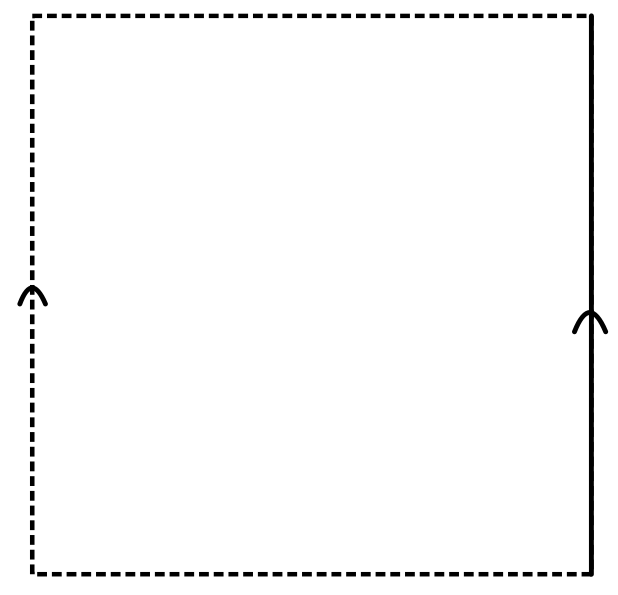
\includegraphics[scale = 0.95]{diagrams/natural_alternating_diagrams/1.png}
    \caption{Your caption here}
    \label{fig:your-label}
\end{figure}


We will specify co-orientations of $i_1, \cdots, i_{n-1}$ so that we can think of the cylindrical closure of the braid word as the the front projection of a Legendrian knot living inside the co-circle bundle of the cylindrical closure.

Let $x_0 \in [0,1]$, we define the co-orientation at $i_k(x_0)$ to be $\xi = adx + cdz$ so that $\xi$ vanishes at $\frac{di_k}{dt}|_{x=x_0}$, $||(a,c)||= 1$, and $c>0$. This can be visually represented as hairs pointing upward(i.e. $c>0$).

\begin{figure}[H] 
    \centering
    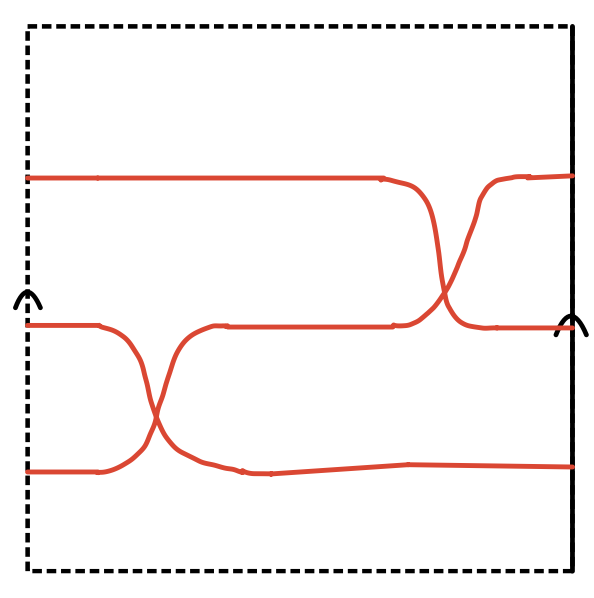
\includegraphics[scale = 0.95]{diagrams/natural_alternating_diagrams/2.png} 
    \caption{Your caption here}
    \label{fig:your-label}
\end{figure}

Suppose we have a Riemann sphere $M$ with two punctures at $0$ and $\infty$. Topologically, $M$ is homeomorphic to the boundaryless cylinder as shown in the figure below.

\begin{figure}[H]
    \centering
    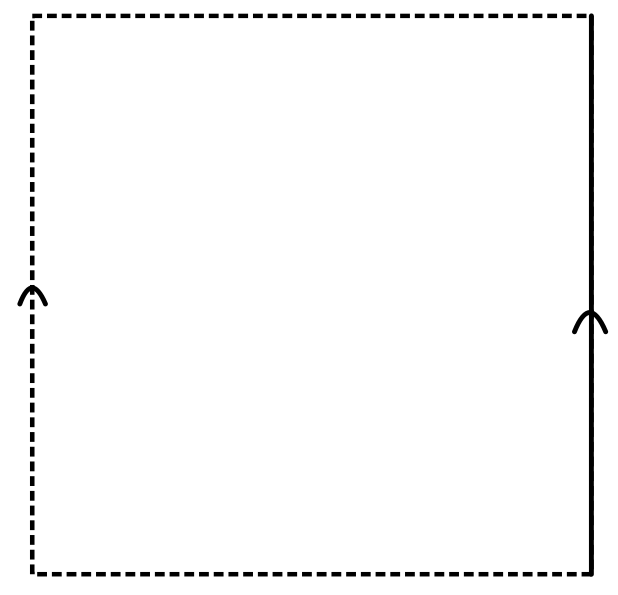
\includegraphics[scale = 0.95]{diagrams/natural_alternating_diagrams/3.png} 
    \caption{Your caption here}
    \label{fig:your-label}
\end{figure}

There are two distinguished ways of embedding the cylindrical closure of $\omega$ into $M$. We can embed the cylindrical closure onto the hemisphere containing $0$($\infty$ resp.), i.e. the lower hemisphere(upper hemisphere resp.), in such a way that the embedding extends

\begin{enumerate}[label = (\roman*)]
\item to $S^1 \times \{ 0 \}$) as an isomophism onto the equator of $M$
\item to  $S^1 \times \{ 1 \}$ as a constant map to $0$($\infty$ resp.)
\end{enumerate}

\begin{figure}[H]
    \centering
    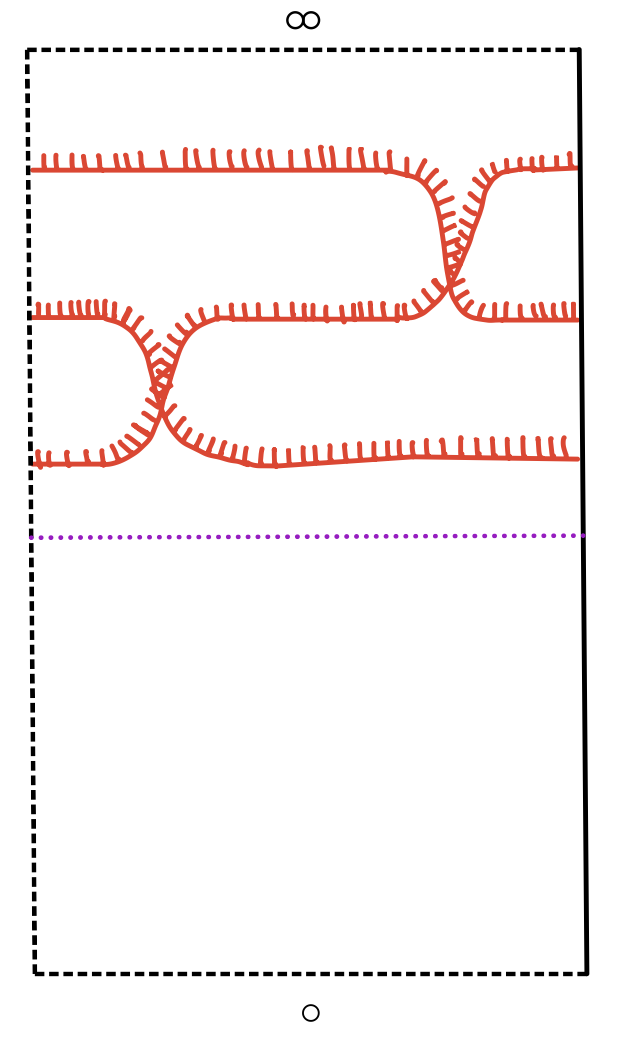
\includegraphics[scale = 0.95]{diagrams/natural_alternating_diagrams/4-1.png} 
    \caption{embedding of the cylindrical closure onto the upper hemisphere}
    \label{fig:your-label}
\end{figure}

\begin{figure}[H] 
    \centering
    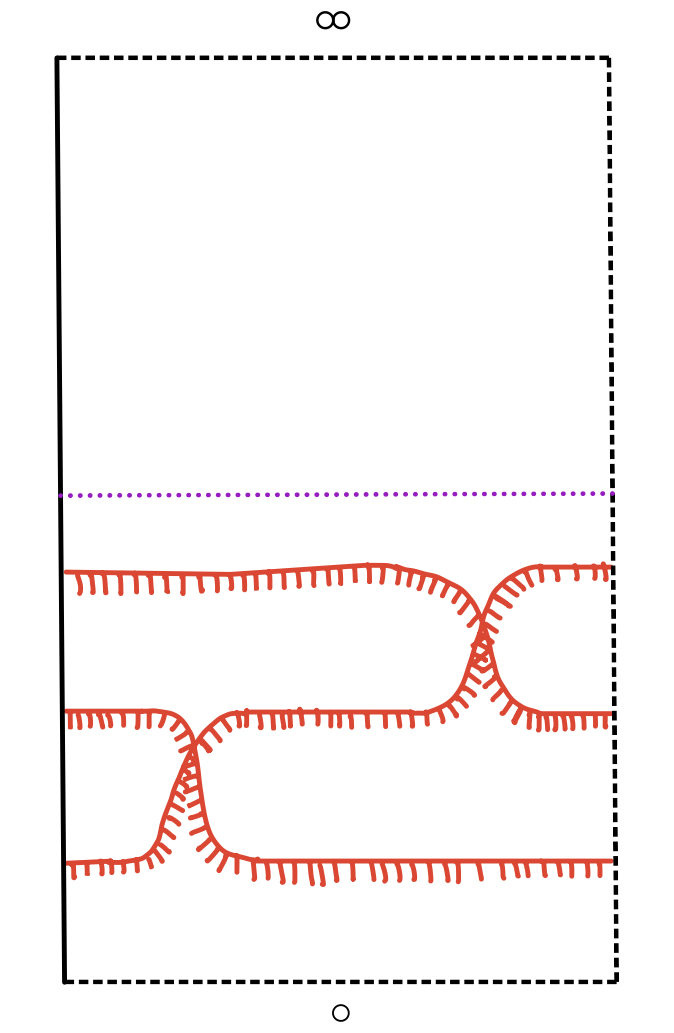
\includegraphics[scale = 0.95]{diagrams/natural_alternating_diagrams/4-2.png} 
    \caption{embedding of the cylindrical closure onto the lower hemisphere}
    \label{fig:your-label}
\end{figure}

Suppose we have a positive braid word $\omega$ on $n$ strands, we have the following associated objects: 
\begin{itemize}
\item $M$: A Riemann sphere with two punctures at $0$ and $\infty$

\item $\Phi_0 : \coprod_{i=1}^{n} S^1 \rightarrow  M$: the front projection induced by the embedding of the cylindrical closure of the trivial braid word onto the lower hemisphere

\item $\xi_0$: the co-orientation of $\Phi_0$

\item $\Phi_\infty : \coprod_{i=1}^{m} S^1 \rightarrow M$ (where $m \leq n$): the front projection given by the embedding of the cylindrical closure of the braid word $\omega$ onto the upper hemisphere

\item $\xi_\infty$ : the co-orientation of $\iota_\infty$
\end{itemize}

To simplify the notation, we will denote the pair $(\Phi_0,\xi_0)$($(\Phi_\infty,\xi_\infty)$ resp.) as $\Lambda_0$($\Lambda_\infty$ resp.). Also, we will abuse $\Lambda_0$($\Lambda_\infty$ resp.) to denote the Legendrian associated to the pair $(\Phi_0,\xi_0)$($(\Phi_\infty,\xi_\infty)$ resp.).

Now fix a positive braid word $\omega$ and the object $(M,\Lambda_0,\Lambda_\infty)$ associated with it which we call the separated diagram of $\omega$. I will define a natural alternating braid diagram $(M,\Lambda'_0,\Lambda'_\infty)$ whose associated Legendrian is Legendrian isotopic to the Legendrian associated with $(M,\Lambda_0,\Lambda_\infty)$. I will construct an explicit Legendrian isotopy between them. Futhermore, I will construct cobordisms between constructible sheaves singular supported on $(M,\Lambda_0,\Lambda_\infty)$ and $(M,\Lambda'_0,\Lambda'_\infty)$ which will be the main result of this chapter. The isotopy will be only applied to $\Lambda_0$, so the $\Lambda_\infty$ will remain fixed i.e. $\Lambda_\infty = \Lambda'_\infty$.

First, let's draw $\Lambda'_\infty$ as in red on $M$ as follows :

\begin{figure}[H] 
    \centering
    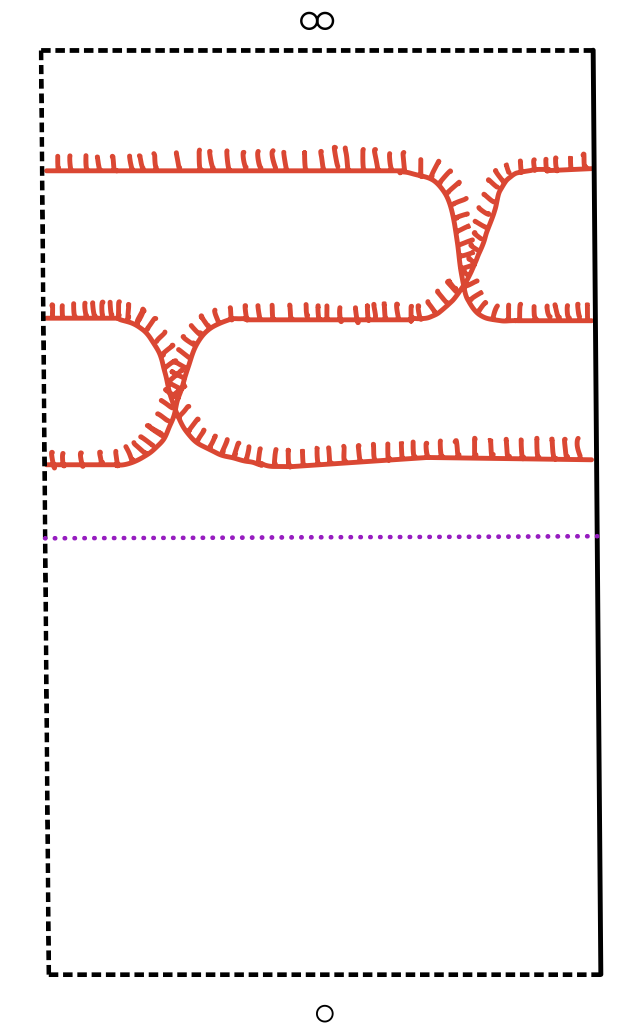
\includegraphics[scale = 0.95]{diagrams/natural_alternating_diagrams/5.png}
    \caption{Your caption here}
    \label{fig:your-label}
\end{figure}

Now on the above diagram, let's draw $\Lambda'_0$ the part that is Legendrian isotopic to $\Lambda_0$ in blue. But before that, we need some definitions.

\begin{definition}
Suppose $\omega = s_{1_1},..., s_{i_k}$, then the cylindirical closure can be parsed into a concatenation of k mutually disjoint regions where $i^{th}$ region containing a part of the braid diagram corresponding to the generator $s_{i_j}$(figure below). We call the region corresponding to $s_{i_j}$ as the $j^{th}$ generator region(also its image under the embedding into $M$).
\end{definition}

Below is the picture of the $1^{st}$ generator region of the cylindrical closure of $\omega = s_1 s_2$.

\begin{figure}[H] 
    \centering
    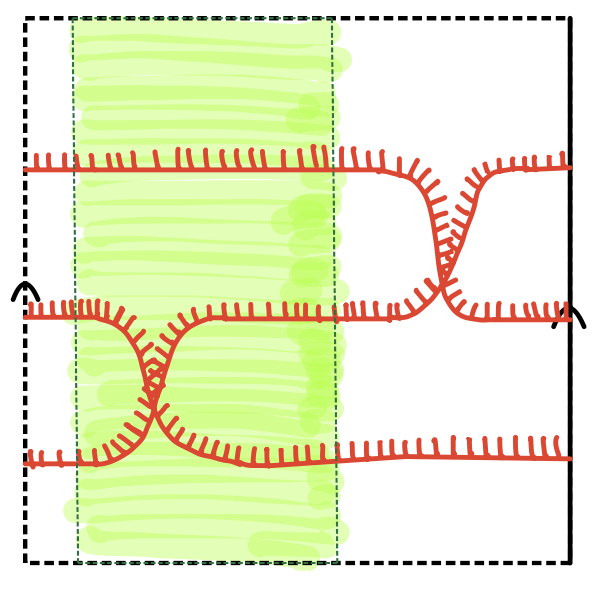
\includegraphics[scale = 0.95]{diagrams/natural_alternating_diagrams/6-1.png}
    \caption{1st generator region}
    \label{fig:your-label}
\end{figure}

Below is the picture of the $2^{nd}$ generator region of the cylindrical closure of $\omega = s_1 s_2$.

\begin{figure}[H] 
    \centering
    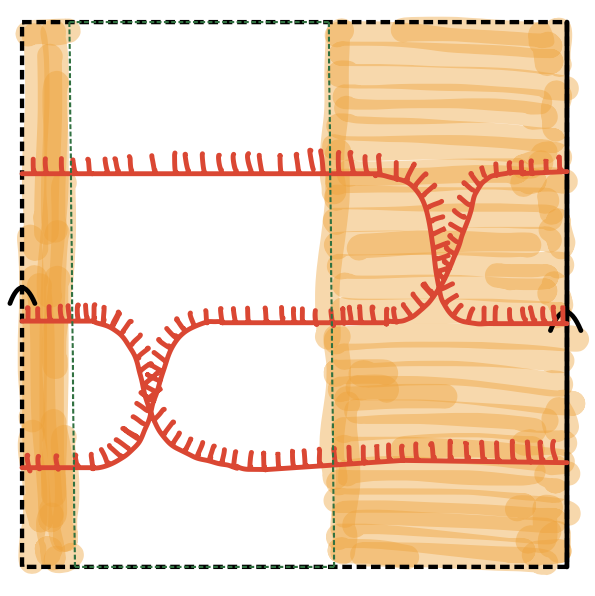
\includegraphics[scale = 0.95]{diagrams/natural_alternating_diagrams/6-2.png}
    \caption{2nd generator region}
    \label{fig:your-label}
\end{figure}

\begin{definition}
Suppose we set-theoretically subtract the union of all generator regions from the cylinder, we get $k$ connected components. That is, for each $j = 1,...,k$, we have one component in between $j^{th}$ and ($j+1$ (mod $k$))$^{th}$ regions. We call the neighborhood of this component inside the cylinder as  $j^{th}$ inter-generator region(also its image inside the cylinder under the embedding into $M$).

\begin{itemize}
\item inter-generator regions do not contain any crossing
\item inter-generator regions are mutually disjoint
\item $j^{th}$ intergenerator region intersects with $j^{th}$ and $j+1^{th}$(modulo $k$) generator region
\end{itemize}
\end{definition}

Below is the picture of the $1^{st}$ inter-generator region of the cylindrical closure of $\omega = s_1 s_2$.

\begin{figure}[H] 
    \centering
    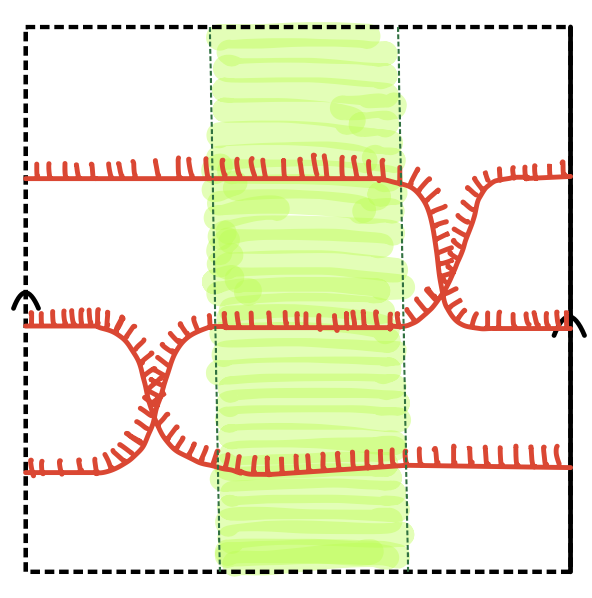
\includegraphics[scale = 0.95]{diagrams/natural_alternating_diagrams/7-1.png}
    \caption{1st inter-generator region}
    \label{fig:your-label}
\end{figure}

Below is the picture of the $2^{nd}$ generator region of the cylindrical closure of $\omega = s_1 s_2$.

\begin{figure}[H]
    \centering
    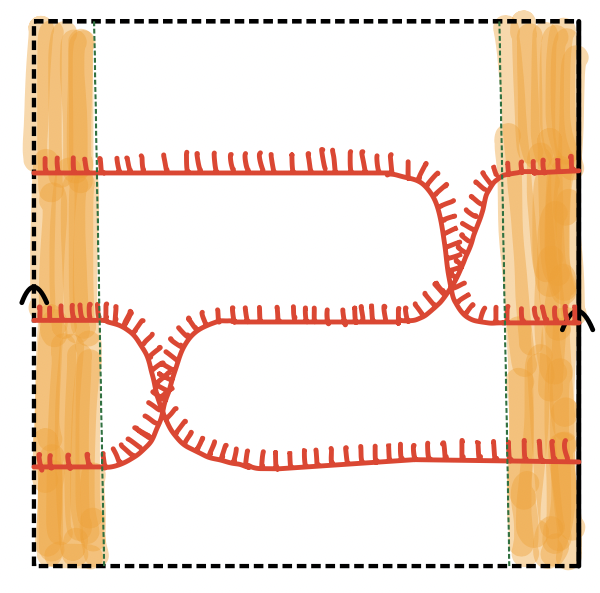
\includegraphics[scale = 0.95]{diagrams/natural_alternating_diagrams/7-2.png}
    \caption{2nd inter-generator region}
    \label{fig:your-label}
\end{figure}

Now I will draw $\Lambda'_0$ for each generator region so that they glue up to the whole $\Lambda'_0$. 

First, we restrict the diagram to $j^{th}$ generator region, we have the following diagram: Note that $i_j^{th}$ and $i_{j}+1^{th}$ strands cross each other and all the other strands are horizontal.

\begin{figure}[H] 
    \centering
    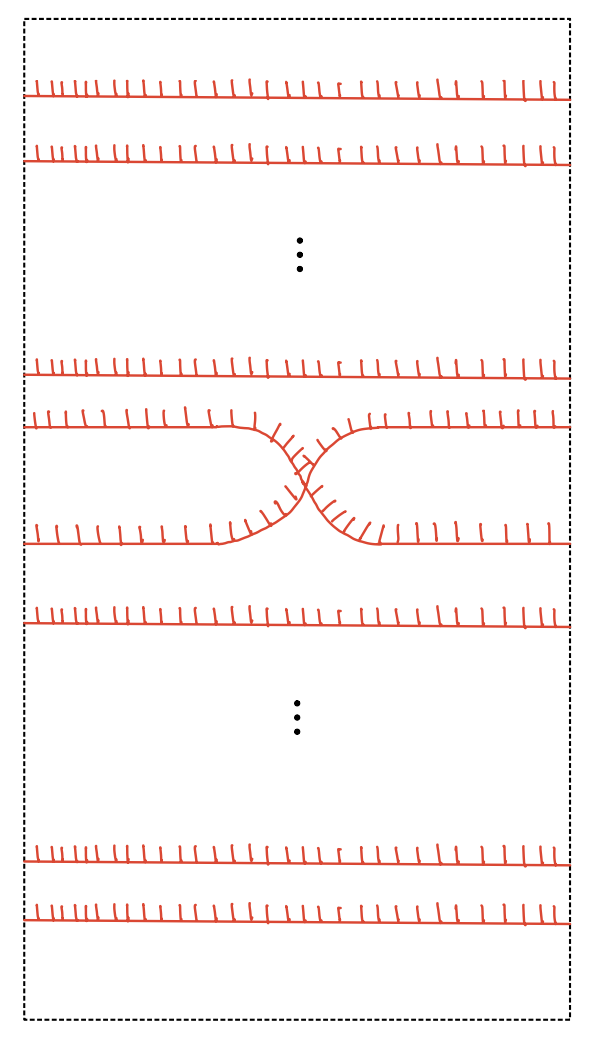
\includegraphics[scale = 0.95]{diagrams/natural_alternating_diagrams/8.png} 
    \caption{Your caption here}
    \label{fig:your-label}
\end{figure}


We label the strands from top to bottom using integers from $1$ to $n$ with reference to the left end points. This is the strand labelling scheme that I will use throughout this chapter.


I will draw $\Lambda'_0$ as blue strand on it as follows :

\begin{itemize}
\item $l^{th}$ blue strand starts from the midpoint of the starting points of $l^{th}$ and $l+1^{th}$ red strands and ends at the midpoint of the end points of $l^{th}$ and $l+1^{th}$ red strands

\item if $l \neq i_j$ and $i\neq i_j +1$, then along the way the $l^{th}$ blue strand crosses up and down once

\item if $l = i_j$, $l^{th}$ blue strand crosses $l^{th}$ red strand up in the part before the crossing and then crosses $l+1^{th}$ red strand down in the part after the crossing.

\item if $l = i_j + 1$, $l^{th}$ blue strand crosses $l+1^{th}$ red strand up and down in the part before the crossing and then crosses $l^{th}$ red strand up and down in the part after the crossing.
\end{itemize}

The picture below overlays $\Lambda'_0$(drawn in blue strands with hairs pointing downward) on the previous diagram(use the precise numbering).

\begin{figure}[H] 
    \centering
    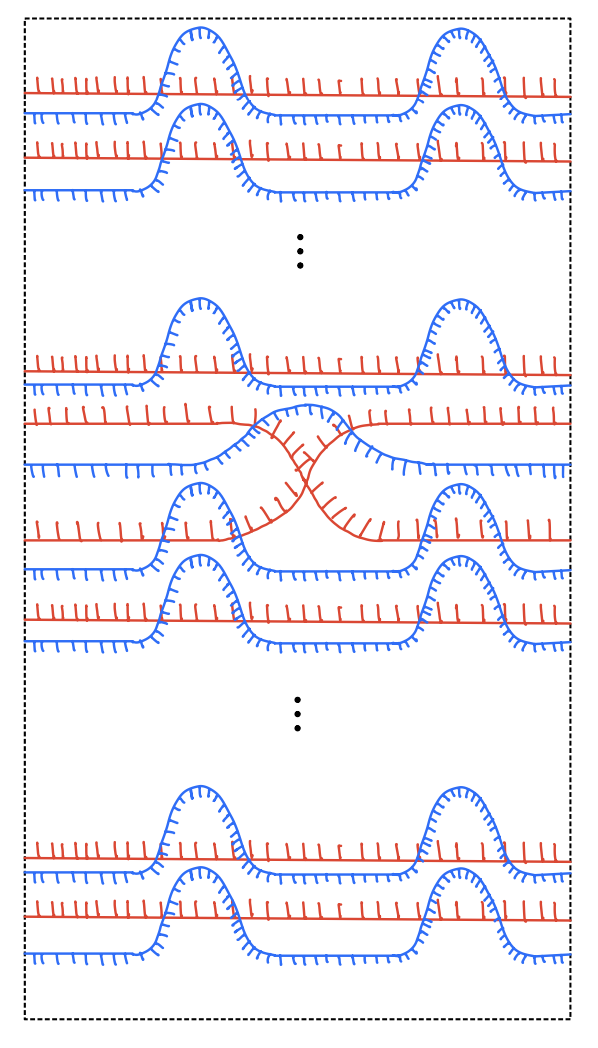
\includegraphics[scale = 0.95]{diagrams/natural_alternating_diagrams/9.png}
    \caption{Your caption here}
    \label{fig:your-label}
\end{figure}

For the full alternating strand diagram, we take the closure of blue strands from the generator regions so that the end points from the bordering regions coincide.

The picture below shows how the global natural alternating strand diagram associated with $\omega = s_1 s_2$ looks like after gluing together local alternating strand diagrams of $s_1$ and $s_2$.

\begin{figure}[H] 
    \centering
    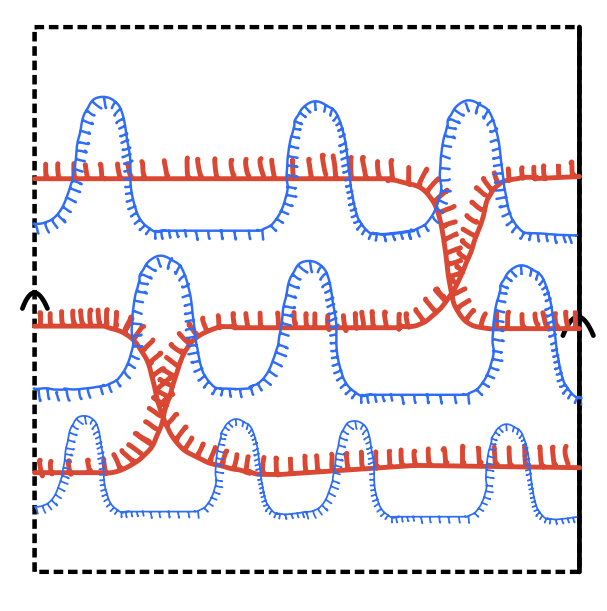
\includegraphics[scale = 0.95]{diagrams/natural_alternating_diagrams/10.png} 
    \caption{Your caption here}
    \label{fig:your-label}
\end{figure}

\begin{theorem}
The above defined strand diagram is alternating
\end{theorem}

\begin{proof}
we will denote
 
\begin{itemize}
\item the region with all the hairs pointing outward as $\circ$
\item the region with all the hairs pointing inward as $\bigtriangleup$
\item else with $\times$
\end{itemize}

for the generator region we have the following figure :

\begin{figure}[H] 
    \centering
    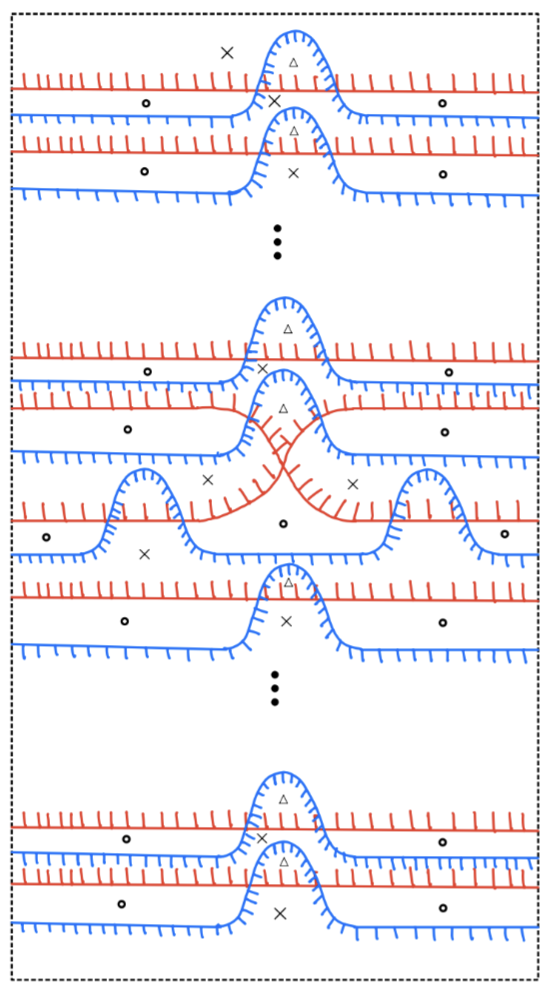
\includegraphics[scale = 0.95]{diagrams/natural_alternating_diagrams/11.png}
    \caption{Your caption here}
    \label{fig:your-label}
\end{figure}

The above marking extends to the inter-generator region, we have the following figure:

\begin{figure}[H] 
    \centering
    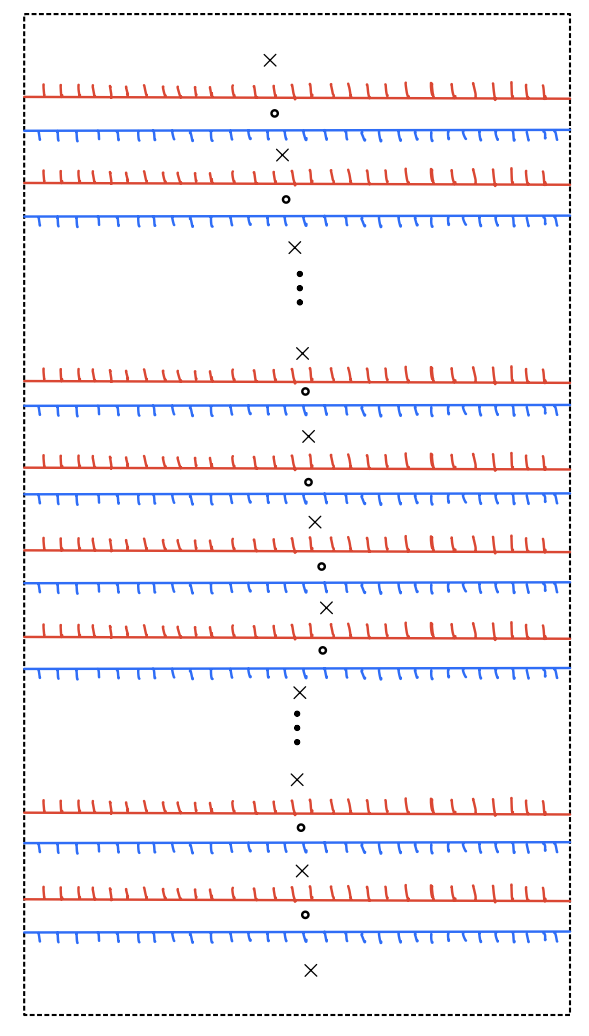
\includegraphics[scale = 0.95]{diagrams/natural_alternating_diagrams/12.png}
    \caption{Your caption here}
    \label{fig:your-label}
\end{figure}

for each crossing, it satisfy the alternating condition. This diagram is indeed alternating.
\end{proof}
\section{local systems on natural alternating diagrams}

Suppose we have a positive braid word $\omega$ then we have the associated natural alternating diagram $(M, \Lambda'_0, \Lambda'_\infty)$ defined in the previous section.

We can associate a quiver $Q$ to the alternating diagram in such a way that

\begin{itemize}
\item we have one vertex for regions where all hairs are pointing outward/inward
\item for each crossing, we have an arrow from the vertex corresponding to the region where all hairs pointing outward to inward
\end{itemize}

For example, for each generator region of a natural alternating strand diagram:

\begin{figure}[H] 
    \centering
    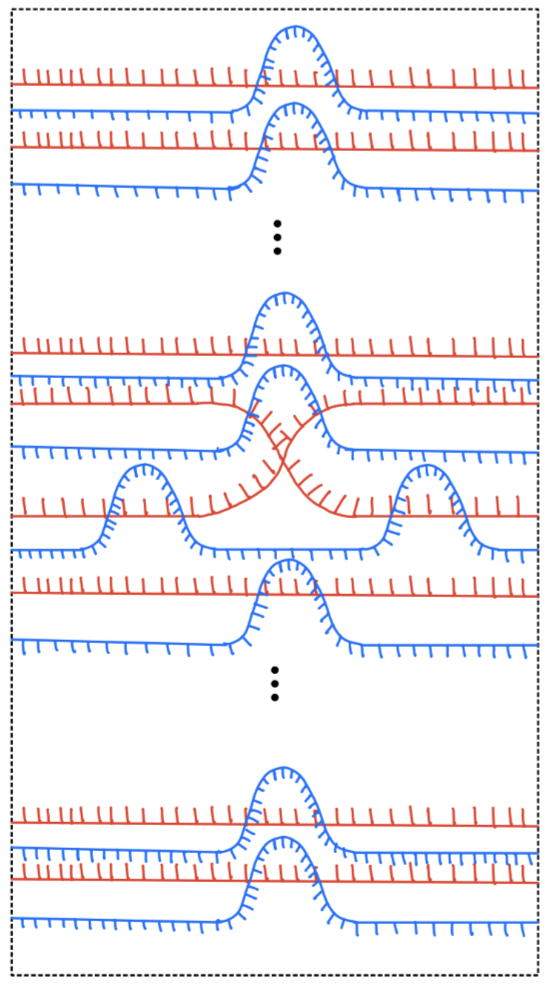
\includegraphics[scale = 0.95]{diagrams/local_systems_on_as_diagrams/1.png} 
    \caption{Your caption here}
    \label{fig:your-label}
\end{figure}

we have the following associated quiver:

\begin{figure}[H] 
    \centering
    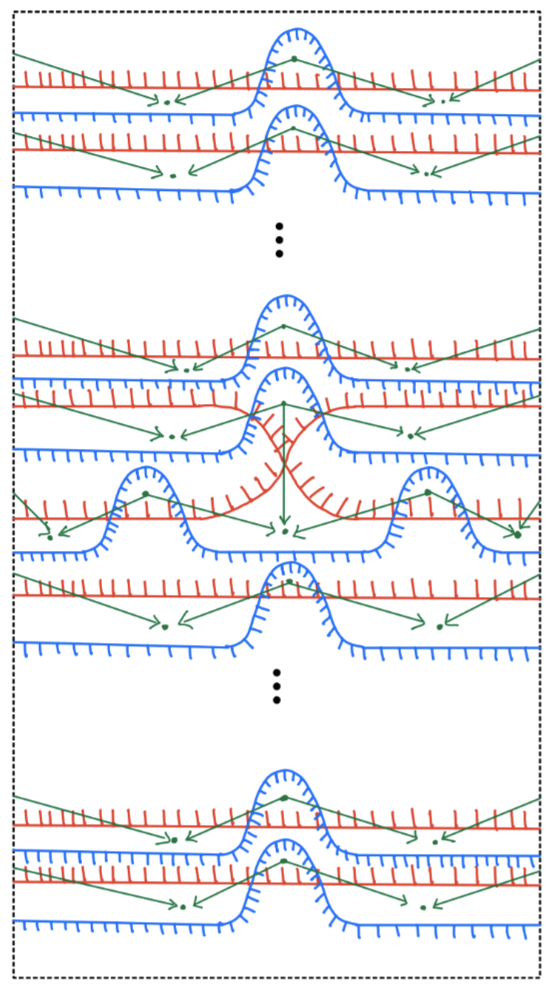
\includegraphics[scale = 0.95]{diagrams/local_systems_on_as_diagrams/2.png} 
    \caption{Your caption here}
    \label{fig:your-label}
\end{figure}

Once we have an alternating strand diagram, we have the associated conjugate surface $S_{conj}$. Furthermore, we can embed the underlying undirected graph of the quiver $Q$(i.e. the bipartite graph of the alternating coloring) in $S_{conj}$ in such a way that $S_{conj}$ deformation retracts to $Q$(with abuse of notation I will denote this underlying undirected graph as $Q$). Suppose we have a rank $1$ local system on the conjugate surface associated with $(M, \Lambda'_0, \Lambda'_\infty)$, then restricting to $Q$, we get a local system on $Q$. Note that the pullback, induced by the restriction map, between the space of local systems $H^1(S_{conj}, \C^*) \rightarrow  H^1(Q,\C^*)$ is an isomorphism.

$H^1(Q,\mathbb{C}^*)$ is isomorphic to $(\C^*)^{|Arr(Q)|}//(\C^*)^{|Vert(Q)|}$
here the group action is defined as the following : let $g_v \in (\C^*)^{|Vert(Q)|}$
(more precisely, $g_v := (g^{\delta_{w,v}})_{w \in Vert(Q)}$ where $\delta$ is the Kronecker delta),
then $g_v \cdot (x_a)_{a\in Arr(Q)}$ is 

\begin{itemize}
\item for entries with index $a$ such that the source of $a$ is $v$ i.e. $s(a) = v$, we have $g_v \cdot x_a$
\item for entries with index $a$ such that the target of $a$ is $v$ i.e. $t(a) = v$, we have $g_v^{-1} \cdot x_a$
\end{itemize}


Now we define the associated alternating sheaf on some regular cell complex refinement of the natural alternating strand diagram associated with a rank $1$ local systems on $Q$.

First, I will describe the special kind of regular cell complex associated with the alternating strand diagram called the regular cell complex refinement of the natural alternating strand diagram. I will define the refinement for each generator region and glue them to get the global regular cell complex.

\begin{definition}
Suppose we fix a generator region for the alternating strand diagram. Then we denote the $j^{th}$ crossing(numbering starts from left to right) the $i^{th}$ blue strand(numbering starts from top to bottom) crosses red strands as $c_{i,j}$. We will call the crossing between $i^{th}$ and $i+1^{th}$ red strand as $c$.
\begin{enumerate}[label = (\roman*)]
\item For each crossing $c_{i,j}$ we add 
\begin{itemize}
\item when $j$ is odd, locally near $c_{i,j}$ we have the following local diagram
\begin{figure}[H] 
    \centering
    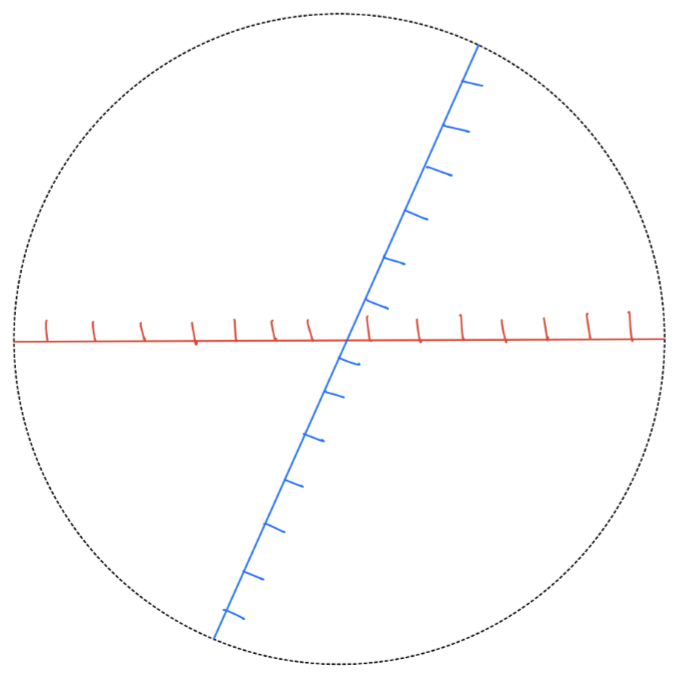
\includegraphics[scale = 0.95]{diagrams/local_systems_on_as_diagrams/3.png} 
    \caption{Your caption here}
    \label{fig:your-label}
\end{figure}
then we add squiggly lines with co-orientations and end points to get
\begin{figure}[H] 
    \centering
    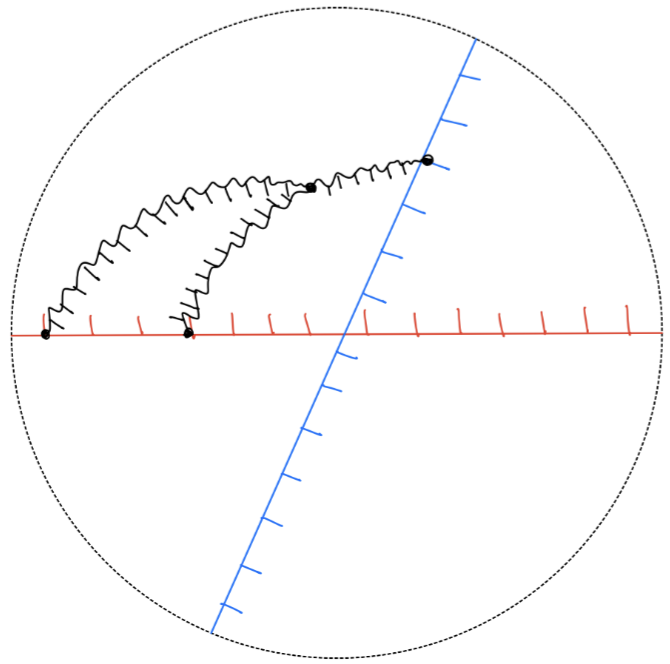
\includegraphics[scale = 0.95]{diagrams/local_systems_on_as_diagrams/4.png} 
    \caption{Your caption here}
    \label{fig:your-label}
\end{figure}
We call the region marked with $*$ a crossing region.
\begin{figure}[H] 
    \centering
    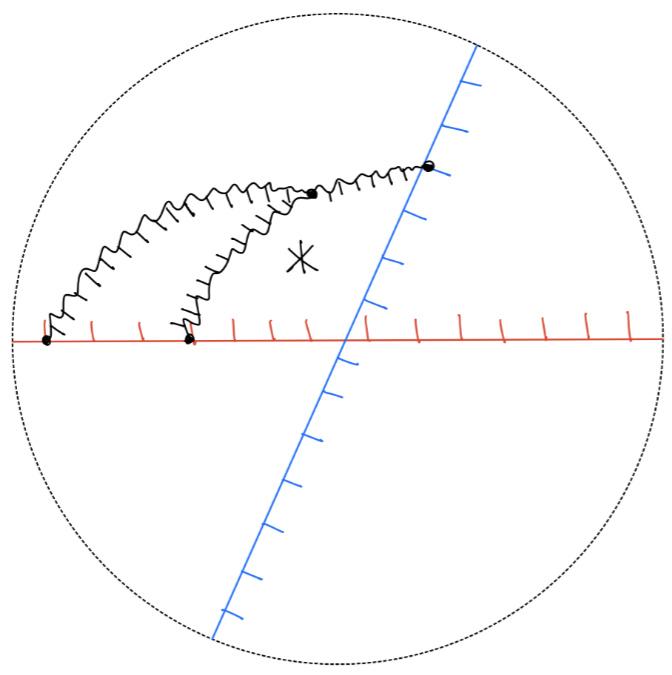
\includegraphics[scale = 0.95]{diagrams/local_systems_on_as_diagrams/5.png} 
    \caption{Your caption here}
    \label{fig:your-label}
\end{figure}

\item when $j$ is even, locally near $c_{i,j}$ we have the following local diagram
\begin{figure}[H] 
    \centering
    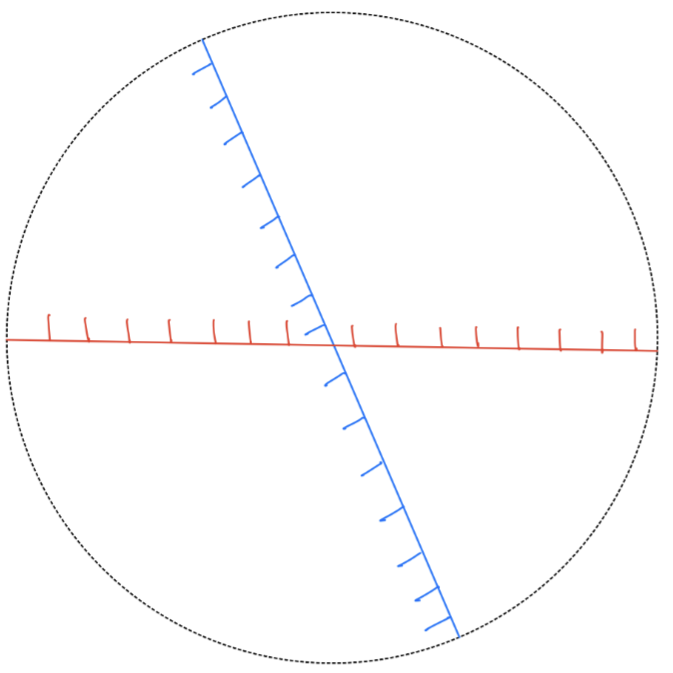
\includegraphics[scale = 0.95]{diagrams/local_systems_on_as_diagrams/6.png} 
    \caption{Your caption here}
    \label{fig:your-label}
\end{figure}
then we add squiggly lines with co-orientations and end points to get
\begin{figure}[H] 
    \centering
    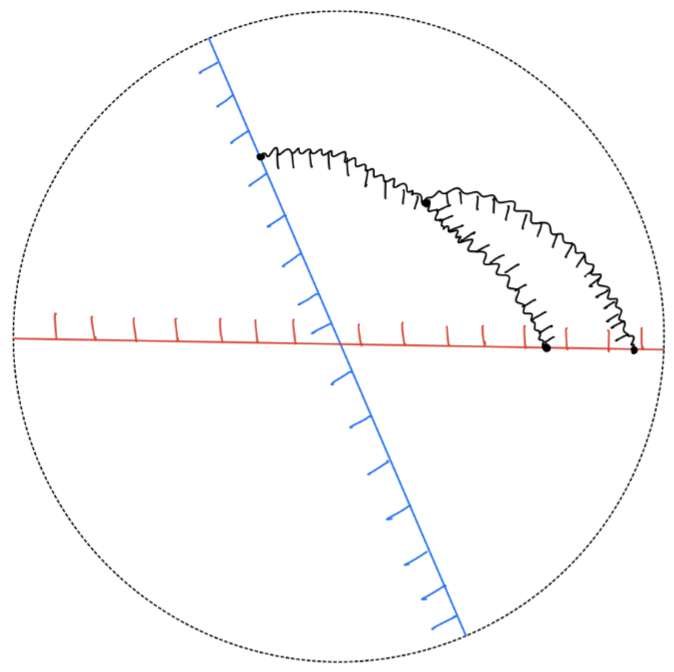
\includegraphics[scale = 0.95]{diagrams/local_systems_on_as_diagrams/7.png} 
    \caption{Your caption here}
    \label{fig:your-label}
\end{figure}
We call the region marked with $*$ a crossing region.
\begin{figure}[H] 
    \centering
    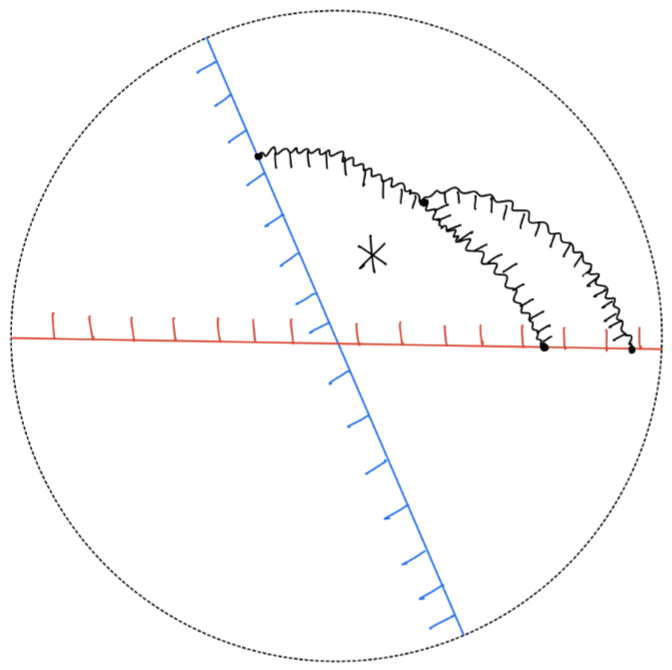
\includegraphics[scale = 0.95]{diagrams/local_systems_on_as_diagrams/8.png} 
    \caption{Your caption here}
    \label{fig:your-label}
\end{figure}
\end{itemize}

\item For the crossing $c$, locally near the crossing, we have the following local diagram
\begin{figure}[H] 
    \centering
    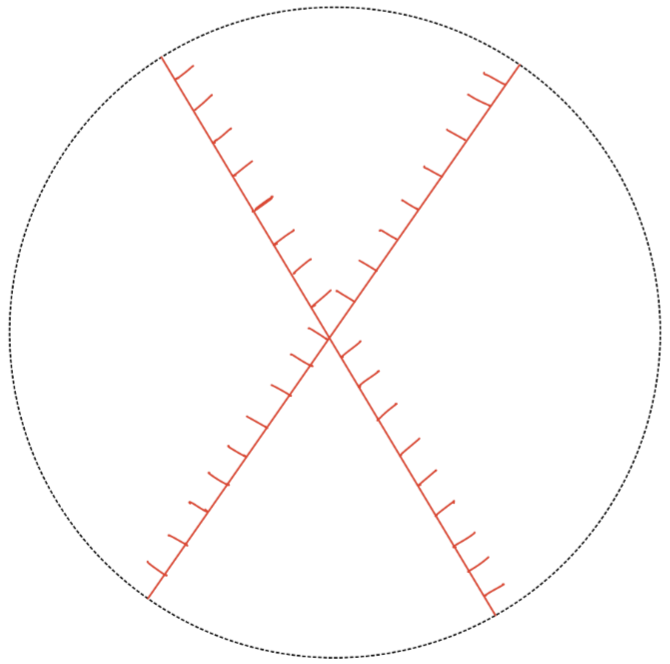
\includegraphics[scale = 0.95]{diagrams/local_systems_on_as_diagrams/9.png} 
    \caption{Your caption here}
    \label{fig:your-label}
\end{figure}
then we add squiggly lines with co-orientations and end points to get
\begin{figure}[H] 
    \centering
    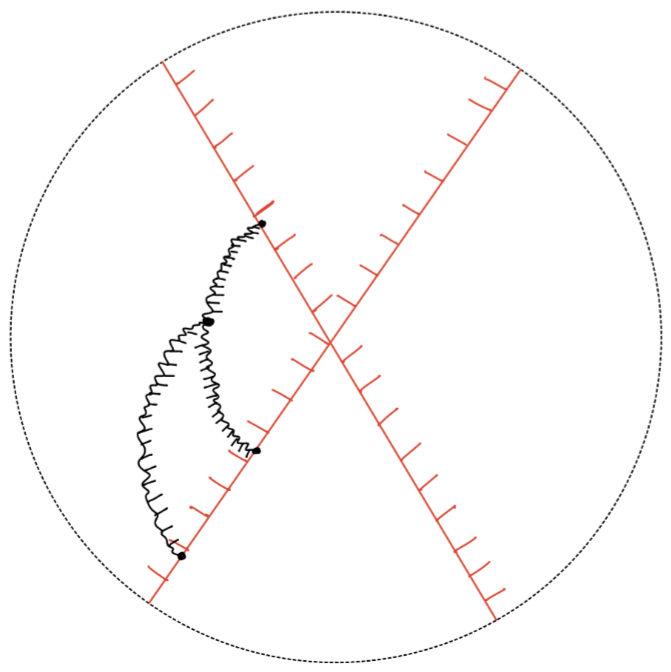
\includegraphics[scale = 0.95]{diagrams/local_systems_on_as_diagrams/10.png} 
    \caption{Your caption here}
    \label{fig:your-label}
\end{figure}
We call the region marked with $*$ a crossing region.
\begin{figure}[H] 
    \centering
    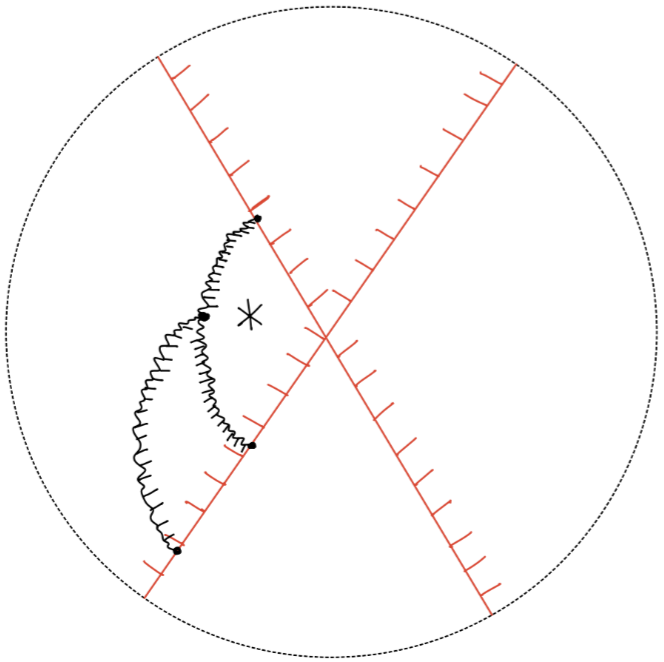
\includegraphics[scale = 0.95]{diagrams/local_systems_on_as_diagrams/11.png} 
    \caption{Your caption here}
    \label{fig:your-label}
\end{figure}
\end{enumerate}

Below is the picture of a generator region of a natural alternating diagram:

\begin{figure}[H] 
    \centering
    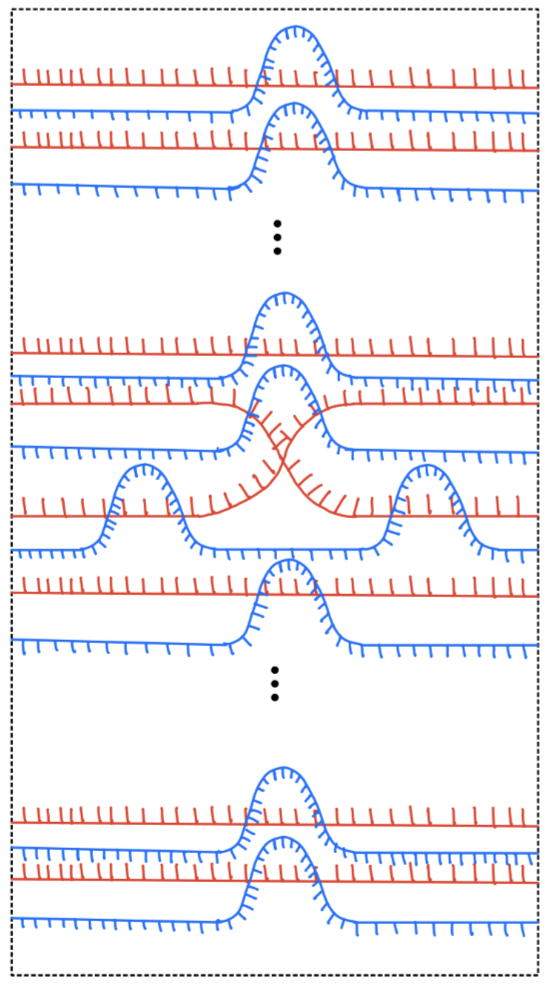
\includegraphics[scale = 0.95]{diagrams/local_systems_on_as_diagrams/12.png} 
    \caption{Your caption here}
    \label{fig:your-label}
\end{figure}

and below is the picture of the regular cell complex refinement in a generator region:

\begin{figure}[H] 
    \centering
    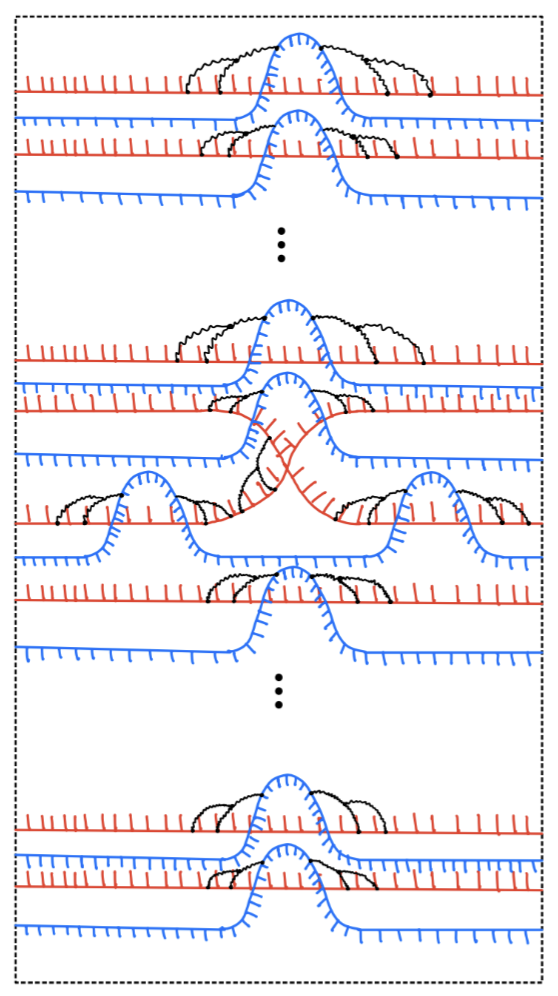
\includegraphics[scale = 0.95]{diagrams/local_systems_on_as_diagrams/13.png}
    \caption{Your caption here}
    \label{fig:your-label}
\end{figure}
\end{definition}
Next, we fix an inter-generator region
\begin{figure}[H] 
    \centering
    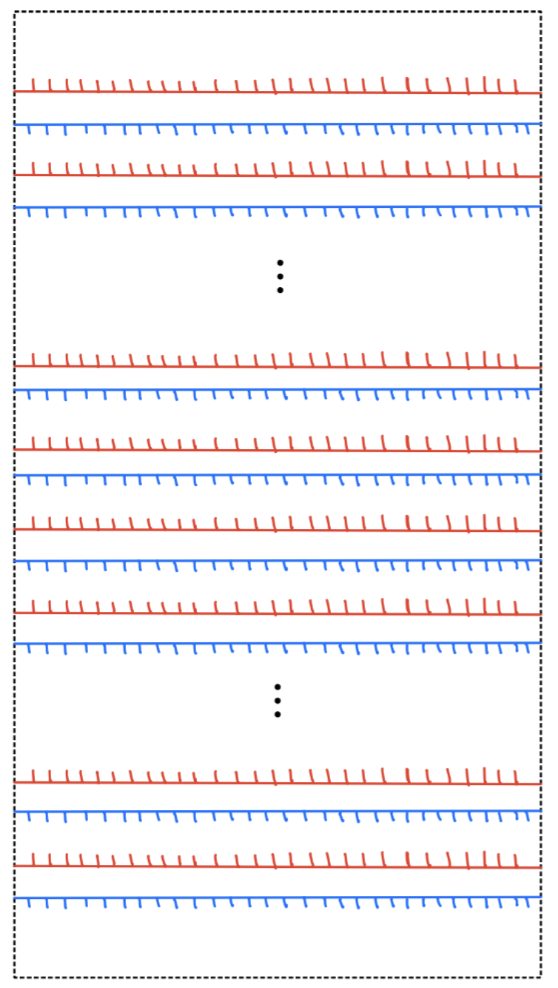
\includegraphics[scale = 0.95]{diagrams/local_systems_on_as_diagrams/14.png} 
    \caption{Your caption here}
    \label{fig:your-label}
\end{figure}

add a vertical squiggly line co-oriented towards the left
\begin{figure}[H] 
    \centering
    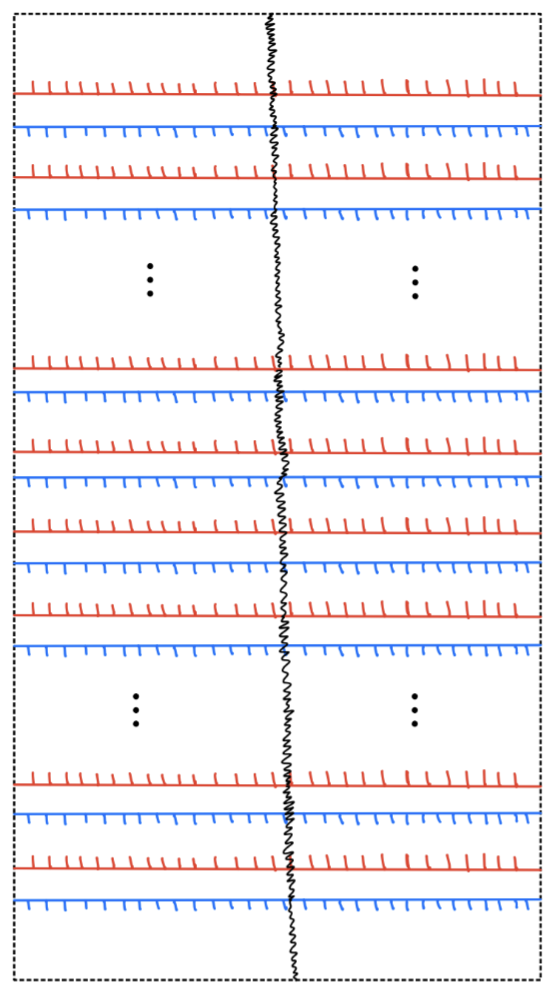
\includegraphics[scale = 0.95]{diagrams/local_systems_on_as_diagrams/15.png} 
    \caption{Your caption here}
    \label{fig:your-label}
\end{figure}


Now I will describe a way to specify a constructible sheaf on the above regular cell complex refinement associated with the local system on $Q$. 

\begin{definition}
Suppose we have a local system on $Q$ which can be represented as an element $(x_A)_{a\in Arr(Q)}(\mathbb{C}^*)^{|Arr(Q)|}$:

\begin{enumerate}[label= (\roman*)]
\item stalk of the region where all the hairs are pointing outward is $\mathbb{C}[-1]$

\item stalk of the region where all the hairs(except the hairs on the squiggly lines) are pointing inward is $\mathbb{C}$

\item stalk of the crossing regions is $\mathbb{C}\xrightarrow{\times x_a}\mathbb{C}$ where $a$ is the arrow corresponding to the associated crossing.

\item rest of the stalks are $0$

\item the only nonzero genrization maps are from regions of type (\Rn{3}) to (\Rn{1}), from (\Rn{1}) to (\Rn{2}), or from (\Rn{2}) to (\Rn{2})(the ones corresponding to vertical squiggly lines in the inter-generator regions)
\end{enumerate}

The maps from (\Rn{3}) to (\Rn{1}) are
\[
  \begin{tikzcd}
    \mathbb{C} \arrow{r}{\times 1} & \mathbb{C} \\
    \mathbb{C}\arrow{u}{} \arrow{r}{}& 0\arrow{u}{}
  \end{tikzcd}
\]

The maps from (\Rn{1}) to (\Rn{2}) are
\[
  \begin{tikzcd}
	0 \arrow{r}{} & \mathbb{C} \\
    \mathbb{C}\arrow{u}{} \arrow{r}{\times 1}& \mathbb{C}\arrow{u}{}
  \end{tikzcd}
\]

The maps from (\Rn{2}) to (\Rn{2}) are identity maps.
\end{definition}

Note that the group action maps a constructible sheaf to the isomorphic constructible sheaf. Therefore, we have a well-defined map
$H^1(S_{conj},\mathbb{C}^*)\rightarrow \mathcal{M}_1((M,\Lambda'_0,\Lambda'_\infty, \Lambda'_{squig}))$ where $\Lambda'_{squig} = (\Phi'_{squig}, \xi'_{squig})$ is the squiggly lines and it's co-orientations in the regular cell complex refinement of the natural alternating diagram.
\section{lemma1}
Suppose we have a Riemann sphere $C$ and two diagrams $(C,\iota,\xi)$ and $(C,\iota',\xi')$ where they differ only in a small disk $D\subset C$. Let $D'$ be a slightly smaller co-centric disk inside $D$. Suppose there is a diffeomorphism between D and $\{(x,y)~|~x^2+y^2 < 4\}$ such that under this diffeomorphism 
\begin{itemize}
\item $D'$ is sent to $\{(x,y)~|~x^2+y^2 < 1\}$
\item the blue strand is sent to a strand that is isotopic to $\{(x,y)~|~y=\frac{1}{2}\}$($\{(x,y)~|~y = \frac{5}{3}x^2 - \frac{3}{4}\}$ resp.)
\item the red strand is sent to a strand that is isotopic to $\{(x,y)~|~y=-\frac{1}{2}\}$($\{(x,y)~|~y=\frac{1}{2}\}$ resp.)
\end{itemize}
Below figures show the diagrams on $D$.


\begin{figure}[H] % Optional: [h] means here, [t] for top, [b] for bottom, [p] for page of floats
    \centering
    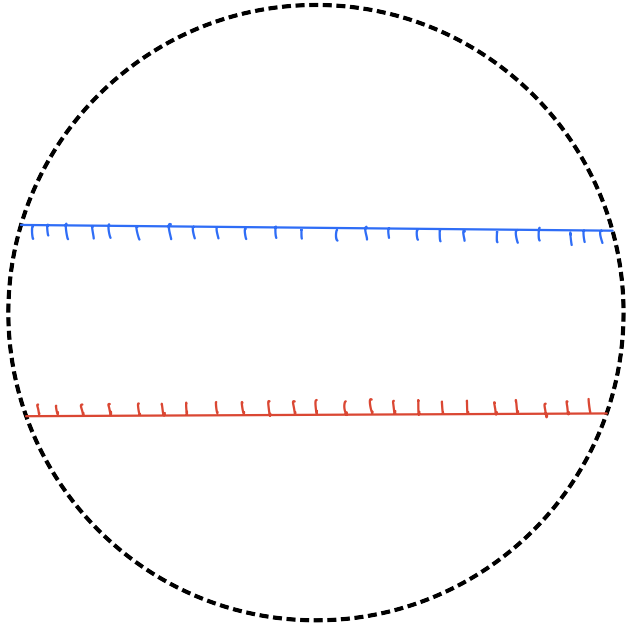
\includegraphics[scale = 0.95]{diagrams/lemma1/1.png} % Adjust the width as needed
    \caption{Your caption here}
    \label{fig:your-label}
\end{figure}


\begin{figure}[H] % Optional: [h] means here, [t] for top, [b] for bottom, [p] for page of floats
    \centering
    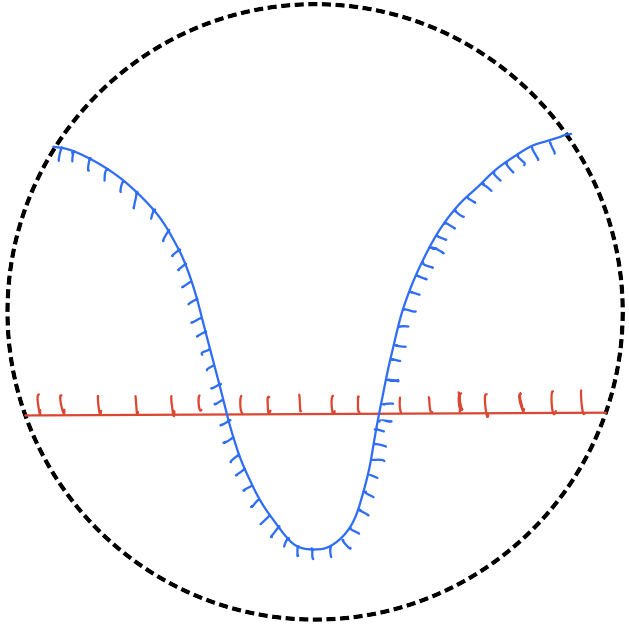
\includegraphics[scale = 0.95]{diagrams/lemma1/2.png} % Adjust the width as needed
    \caption{Your caption here}
    \label{fig:your-label}
\end{figure}

$isotopy_1$ defined in Definition1 defines an isotopy from $(C,\iota,\xi)$ to $(C,\iota',\xi')$. It defines a map $\mathcal{M}_{(C,\iota,\xi)}\rightarrow \mathcal{M}_{(C,\iota',\xi')}$. Under this map, a sheaf on $(C,\iota,\xi)$ described in the figure3 below is mapped to the sheaf on $(C,\iota',\xi')$ described in the figure4 below(figures below show only on $D$ where they differ because the stalks and generization maps away from the region remains the same).

\begin{figure}[H] % Optional: [h] means here, [t] for top, [b] for bottom, [p] for page of floats
    \centering
    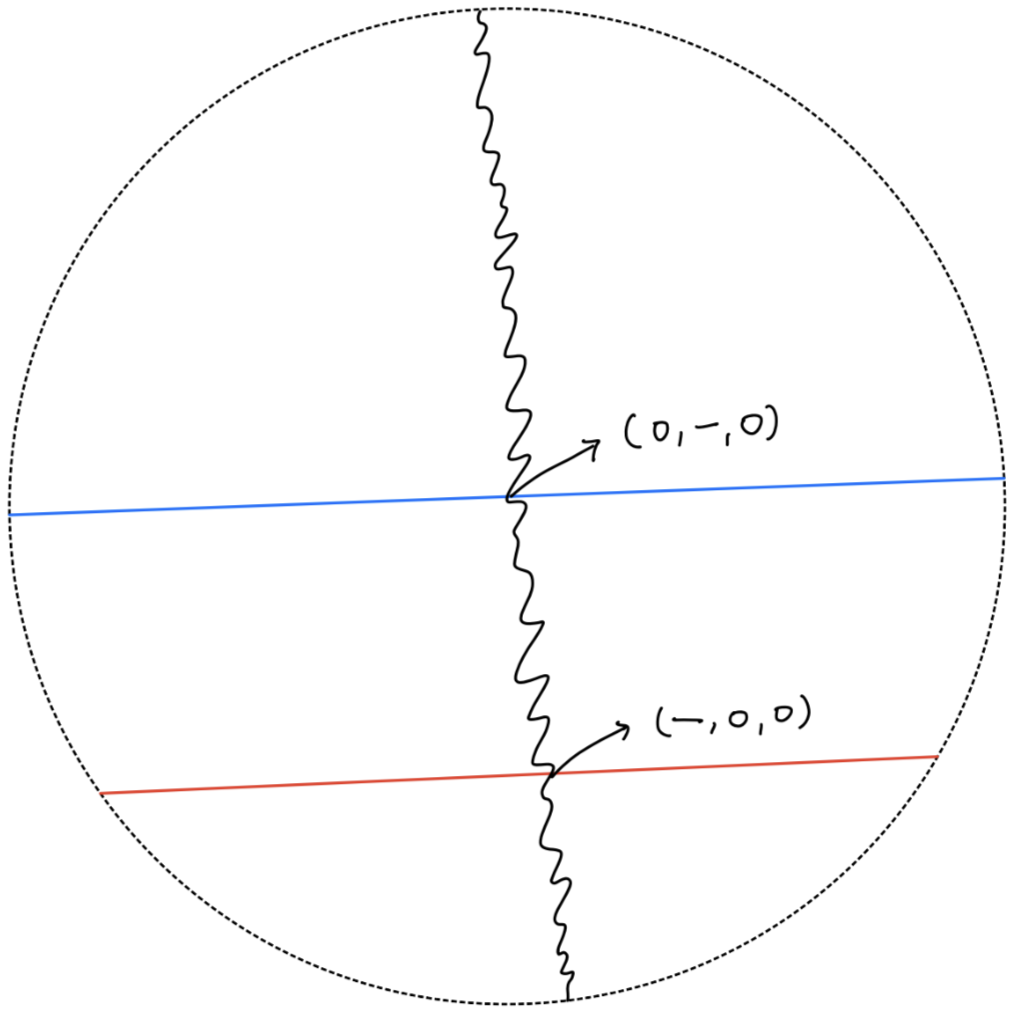
\includegraphics[scale = 0.95]{diagrams/lemma1/3.png} % Adjust the width as needed
    \caption{Your caption here}
    \label{fig:your-label}
\end{figure}
Stalks :
\begin{itemize}
\item $1$ : $\mathbb{C}^{m+1}$
\item $2$ : $\mathbb{C}^{m}$
\item $3$ : $\mathbb{C}^{m+1}$
\end{itemize}
Generization maps :
\begin{itemize}
\item $2\rightarrow 1$ : $\mathbb{C}^{m}\rightarrow \mathbb{C}^{m+1}$ where $e_i\mapsto e_{i+1}$
\item $2\rightarrow 3$ : $\mathbb{C}^{m}\rightarrow \mathbb{C}^{m+1}$ where $e_i\mapsto e_{i}$
\end{itemize}

\begin{figure}[H] % Optional: [h] means here, [t] for top, [b] for bottom, [p] for page of floats
    \centering
    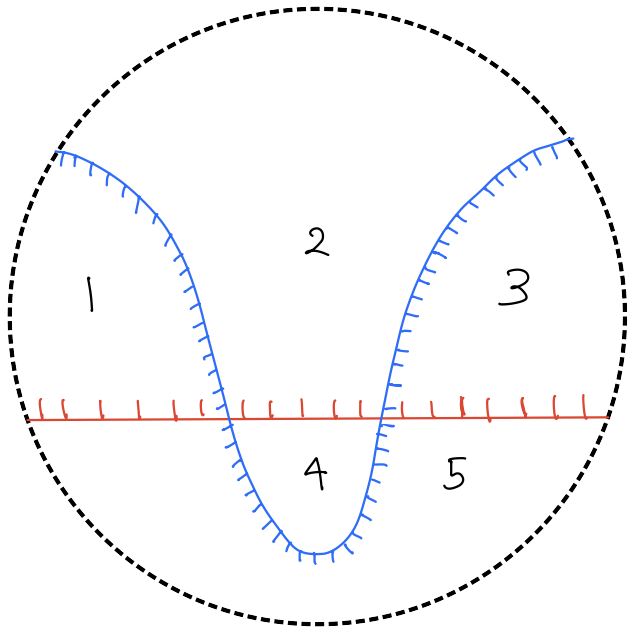
\includegraphics[scale = 0.95]{diagrams/lemma1/4.png} % Adjust the width as needed
    \caption{Your caption here}
    \label{fig:your-label}
\end{figure}

Stalks :
\begin{itemize}
\item $1$ : $\mathbb{C}^{m}$
\item $2$ : $\mathbb{C}^{m+1}$
\item $3$ : $\mathbb{C}^{m}$
\item $4$ : $\mathbb{C}^{m+2}$
\item $5$ : $\mathbb{C}^{m+1}$
\end{itemize}
Generization maps :
\begin{itemize}
\item $1\rightarrow 2$ : $\mathbb{C}^{m}\rightarrow \mathbb{C}^{m+1}$ where $e_i\mapsto e_{i+1}$
\item $3\rightarrow 2$ : $\mathbb{C}^{m}\rightarrow \mathbb{C}^{m+1}$ where $e_i\mapsto e_{i+1}$
\item $1\rightarrow 5$ : $\mathbb{C}^{m}\rightarrow \mathbb{C}^{m+1}$ where $e_i\mapsto e_{i}$
\item $3\rightarrow 5$ : $\mathbb{C}^{m}\rightarrow \mathbb{C}^{m+1}$ where $e_i\mapsto e_{i}$
\item $5\rightarrow 4$ : $\mathbb{C}^{m+1}\rightarrow \mathbb{C}^{m+2}$ where $e_i\mapsto e_{i+1}$
\item $2\rightarrow 4$ : $\mathbb{C}^{m+!}\rightarrow \mathbb{C}^{m+2}$ where $e_i\mapsto e_{i}$
\end{itemize}

(proof)
\section{lemma2(core)}

\begin{lemma}
\end{lemma}
Suppose we have a Riemann Sphere $C$ and two diagrams $(C,\iota,\xi)$,$(C',\iota',\xi')$, their regular cell complex refinements $\overline{(C,\iota,\xi)}$,$\overline{(C',\iota',\xi')}$ and sheaves $\mathfrak{F}$,$\mathfrak{F}'$ on them such that they differ only on a small disk $D\subset C$.\\

Below figures show only $\mathfrak{F}$,$\mathfrak{F}'$ restricted to $D$.
\begin{figure}[H] % Optional: [h] means here, [t] for top, [b] for bottom, [p] for page of floats
    \centering
    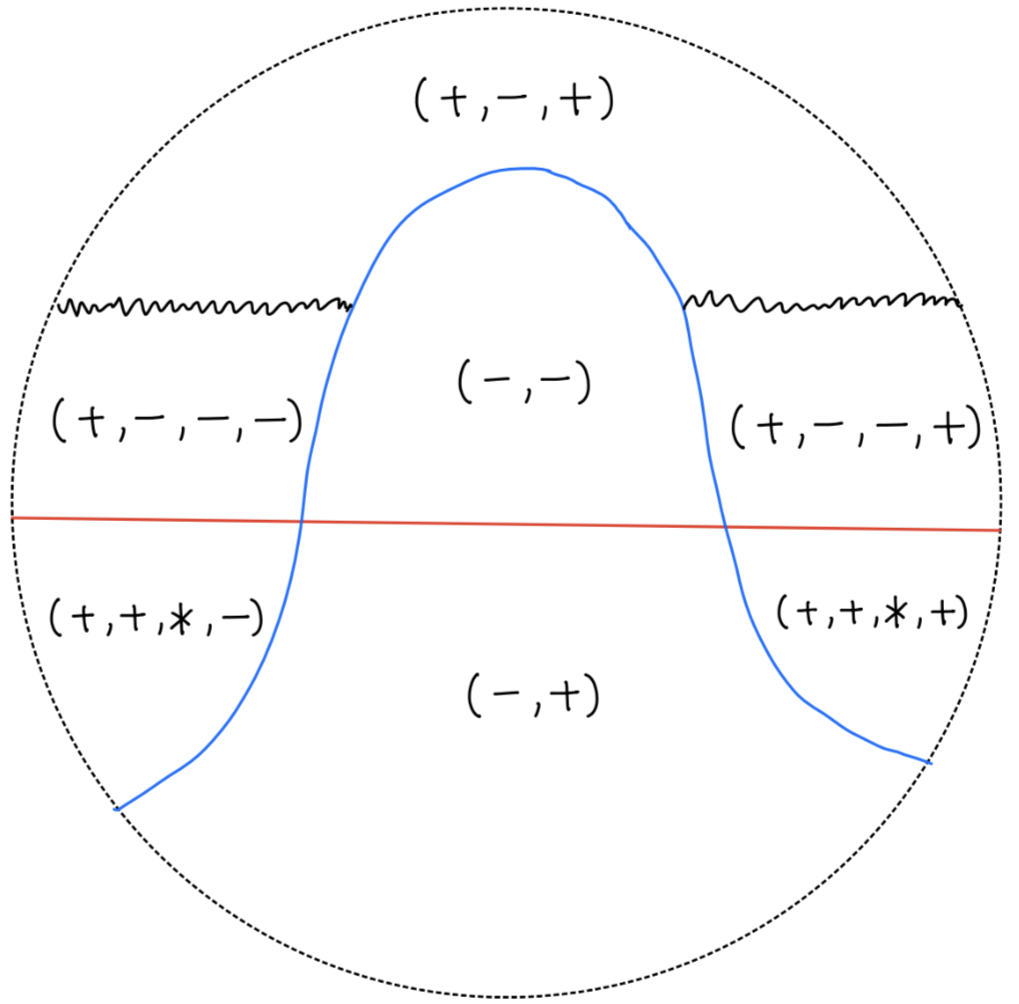
\includegraphics[scale = 0.95]{diagrams/lemma2/1.png} % Adjust the width as needed
    \caption{Your caption here}
    \label{fig:your-label}
\end{figure}

Stalks : \\
- 1 : 0\\
- 2 : $\mathbb{C}\xrightarrow{\times a}\mathbb{C}$\\
- 3 : $\mathbb{C}\xrightarrow{\times b}\mathbb{C}$\\
- 4 : $\mathbb{C}[-1]$ \\
- 5 : $\mathbb{C}$\\
- 6 : $\mathbb{C}$\\
- 7 : 0\\

Generization maps : \\
- 4$\rightarrow$ 1 : zero map \\
- 2$\rightarrow$ 1 : zero map \\
- 3$\rightarrow$ 1 : zero map \\
- 1$\rightarrow$ 5 : zero map \\
- 1$\rightarrow$ 6 : zero map \\
- 7$\rightarrow$ 5 : zero map \\
- 7$\rightarrow$ 6 : zero map \\
- 4$\rightarrow$ 2: 
\begin{tikzcd}
\mathbb{C} \arrow[r, "id"]     & \mathbb{C}  \\
0 \arrow[r]\arrow[u,] & \mathbb{C} \arrow[u,"\times a"]
\end{tikzcd}

- 4$\rightarrow$ 3: 
\begin{tikzcd}
\mathbb{C} \arrow[r, "id"]     & \mathbb{C}  \\
0 \arrow[r]\arrow[u,] & \mathbb{C} \arrow[u,"\times b"]
\end{tikzcd}

- 2$\rightarrow$ 5: 
\begin{tikzcd}
\mathbb{C} \arrow[r,]     & 0  \\
\mathbb{C} \arrow[r, "id"]\arrow[u,"\times a"] & \mathbb{C} \arrow[u,]
\end{tikzcd}

- 3$\rightarrow$ 6: 
\begin{tikzcd}
\mathbb{C} \arrow[r,]     & 0  \\
\mathbb{C} \arrow[r, "id"]\arrow[u,"\times b"] & \mathbb{C} \arrow[u,]
\end{tikzcd}

\begin{figure}[H] % Optional: [h] means here, [t] for top, [b] for bottom, [p] for page of floats
    \centering
    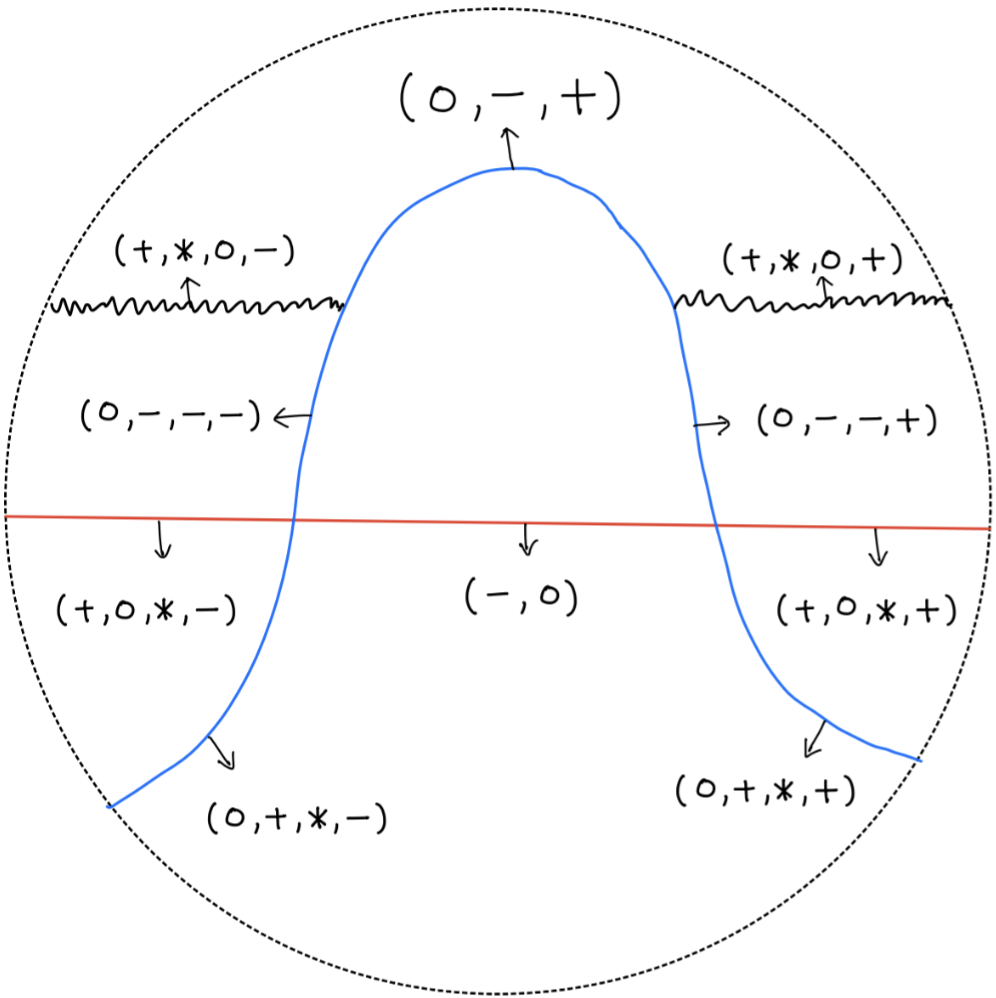
\includegraphics[scale = 0.95]{diagrams/lemma2/2.png} % Adjust the width as needed
    \caption{Your caption here}
    \label{fig:your-label}
\end{figure}

Stalks : \\
1 : 0 \\
2 : $\mathbb{C}\xrightarrow{\times a}\mathbb{C}$\\
3 : $\mathbb{C}\xrightarrow{\times b}\mathbb{C}$\\
4 : $\mathbb{C}$ \\
5 : $\mathbb{C}$ \\
6 : 0

Generization maps : \\

2$\rightarrow$1 : zero map \\
3$\rightarrow$1 : zero map \\
6$\rightarrow$4 : zero map \\
6$\rightarrow$5 : zero map \\
2$\rightarrow$ 4: 
\begin{tikzcd}
\mathbb{C} \arrow[r,]     & 0  \\
\mathbb{C} \arrow[r, "id"]\arrow[u,"\times a"] & \mathbb{C} \arrow[u,]
\end{tikzcd}
\\

3$\rightarrow$ 5: 
\begin{tikzcd}
\mathbb{C} \arrow[r,]     & 0  \\
\mathbb{C} \arrow[r, "id"]\arrow[u,"\times b"] & \mathbb{C} \arrow[u,]
\end{tikzcd}

4$\rightarrow$ 5: $\mathbb{C}\xrightarrow{\times ab^{-1}}\mathbb{C}$\\

We define an isotopy between $\mathfrak{F}$ and $\mathfrak{F}'$ called $isotopy_2$ as follows :

$(\Rn{1})$ The trajectory of the red strand in $D\times [0,1]$ is $\{(x,y,t)\in D\times [0,1]~|~ y = \frac{1}{2}\}$\\
$(\Rn{2})$ The trajectory of blue strand in $D\times [0,1]$ is $\{(x,y,t)\in D\times [0,1]~|~ y = \frac{5}{3}(t-1)x^2 - \frac{5}{4} + \frac{3}{4}\}$. Note that when $t=t_0$, the above set is a parabola passing through $(-\frac{\sqrt{3}}{2}, -\frac{1}{2})$, $(\frac{\sqrt{3}}{2}, -\frac{1}{2})$, $(0, \frac{5}{4}t_0 + \frac{3}{4})$\\

$(\Rn{3})$ The trajectory of the left squiggly line is $\{(x,y,t)\in D\times [0,1]~|~y = \sqrt{\frac{1}{16}-(x+\frac{1}{4})^2}, y \geq \frac{5}{3}(t-1)x^2 - \frac{5}{4}t + \frac{3}{4} \}$\\

$(\Rn{4})$ The trajectory of the right squiggly line $\{(x,y,t)\in D\times [0,1]~|~y = \sqrt{\frac{1}{16}-(x-\frac{1}{4})^2}, y \geq \frac{5}{3}(t-1)x^2 - \frac{5}{4}t + \frac{3}{4} \}$\\

$(\Rn{5})$ The trajectory of the middle squiggly line is$\{(x,y,t)\in D\times [0,1]~|~x=0,y\geq -\frac{1}{2}, y \leq -\frac{5}{4}t + \frac{3}{4} \}$\\

Now I will define sheaf on $D\times [0,1]$ singular supported on $(\Rn{1},\cdots,\Rn{5})$ such that restricted to $D\times\{0\}$($D\times\{1\}$ resp.) is $\mathfrak{F}$($\mathfrak{F}'$ resp.)\\

We can describe the sheaf by assigning stalks to the 7 regions separated by $(\Rn{1},\cdots,\Rn{5})$ and generization maps between them.\\

Let's list the seven regions :

region 1.$\{(x,y,t)\in D\times [0,1]~|~y \geq \sqrt{\frac{1}{16}-(x+\frac{1}{4})^2}, y \geq \sqrt{\frac{1}{16}-(x-\frac{1}{4})^2}, y\geq \frac{1}{2} \}$\\

region2. $\{(x,y,t)\in D\times [0,1]~|~y \geq \frac{5}{3}(t-1)x^2 - \frac{5}{4}t + \frac{3}{4}, y \leq \sqrt{\frac{1}{16}-(x+\frac{1}{4})^2}, y\geq \frac{1}{2} \}$\\

region3. $\{(x,y,t)\in D\times [0,1]~|~y \geq \frac{5}{3}(t-1)x^2 - \frac{5}{4}t + \frac{3}{4}, y \leq \sqrt{\frac{1}{16}-(x-\frac{1}{4})^2}, y\geq \frac{1}{2} \}$\\

region4. $\{(x,y,t)\in D\times [0,1]~|~y \leq \frac{5}{3}(t-1)x^2 - \frac{5}{4}t + \frac{3}{4}, y\geq \frac{1}{2} \}$\\

region5. $\{(x,y,t)\in D\times [0,1]~|~y \geq \frac{5}{3}(t-1)x^2 - \frac{5}{4}t + \frac{3}{4},  y\leq \frac{1}{2}, x\leq 0 \}$\\

region6. $\{(x,y,t)\in D\times [0,1]~|~y \geq \frac{5}{3}(t-1)x^2 - \frac{5}{4}t + \frac{3}{4},  y\leq \frac{1}{2}, x\geq 0 \}$\\

region7. $\{(x,y,t)\in D\times [0,1]~|~y \leq \frac{5}{3}(t-1)x^2 - \frac{5}{4}t + \frac{3}{4},  y\leq \frac{1}{2} \}$\\

Now let's define \\

Stalks:\\

- 1 : 0\\
- 2 : $\mathbb{C}\xrightarrow{\times a}\mathbb{C}$\\
- 3 : $\mathbb{C}\xrightarrow{\times b}\mathbb{C}$\\
- 4 : $\mathbb{C}[-1]$ \\
- 5 : $\mathbb{C}$\\
- 6 : $\mathbb{C}$\\
- 7 : 0\\ 


Generization maps :\\
- 4$\rightarrow$ 1 : zero map \\
- 2$\rightarrow$ 1 : zero map \\
- 3$\rightarrow$ 1 : zero map \\
- 1$\rightarrow$ 5 : zero map \\
- 1$\rightarrow$ 6 : zero map \\
- 7$\rightarrow$ 5 : zero map \\
- 7$\rightarrow$ 6 : zero map \\
- 4$\rightarrow$ 2: 
\begin{tikzcd}
\mathbb{C} \arrow[r, "id"]     & \mathbb{C}  \\
0 \arrow[r]\arrow[u,] & \mathbb{C} \arrow[u,"\times a"]
\end{tikzcd}

- 4$\rightarrow$ 3: 
\begin{tikzcd}
\mathbb{C} \arrow[r, "id"]     & \mathbb{C}  \\
0 \arrow[r]\arrow[u,] & \mathbb{C} \arrow[u,"\times b"]
\end{tikzcd}

- 2$\rightarrow$ 5: 
\begin{tikzcd}
\mathbb{C} \arrow[r,]     & 0  \\
\mathbb{C} \arrow[r, "id"]\arrow[u,"\times a"] & \mathbb{C} \arrow[u,]
\end{tikzcd}

- 3$\rightarrow$ 6: 
\begin{tikzcd}
\mathbb{C} \arrow[r,]     & 0  \\
\mathbb{C} \arrow[r, "id"]\arrow[u,"\times b"] & \mathbb{C} \arrow[u,]
\end{tikzcd}

- 5$\rightarrow$ 6: $\mathbb{C}\xrightarrow{\times ab^{-1}}\mathbb{C}$\\

Below we will prove that this is a well-defined isotopy between $\mathfrak{F}$ and $\mathfrak{F}'$.\\

(proof of well-definedness)
\section{lemma3(core)}
\begin{lemma}
\end{lemma}
Suppose we have a Riemann sphere $C$ and two diagrams $(C,\iota,\xi)$,$(C,\iota',\xi')$ and their refinements $\overline{(C,\iota,\xi)}$,$\overline{(C,\iota',\xi')}$ and sheaves $\mathfrak{F}$,$\mathfrak{F}'$ on them such that they differ only on a small disk $D\subset C$. \\

Below figures show only $\mathfrak{F}$, $\mathfrak{F}'$ restricted to $D$.


\begin{figure}[H] % Optional: [h] means here, [t] for top, [b] for bottom, [p] for page of floats
    \centering
    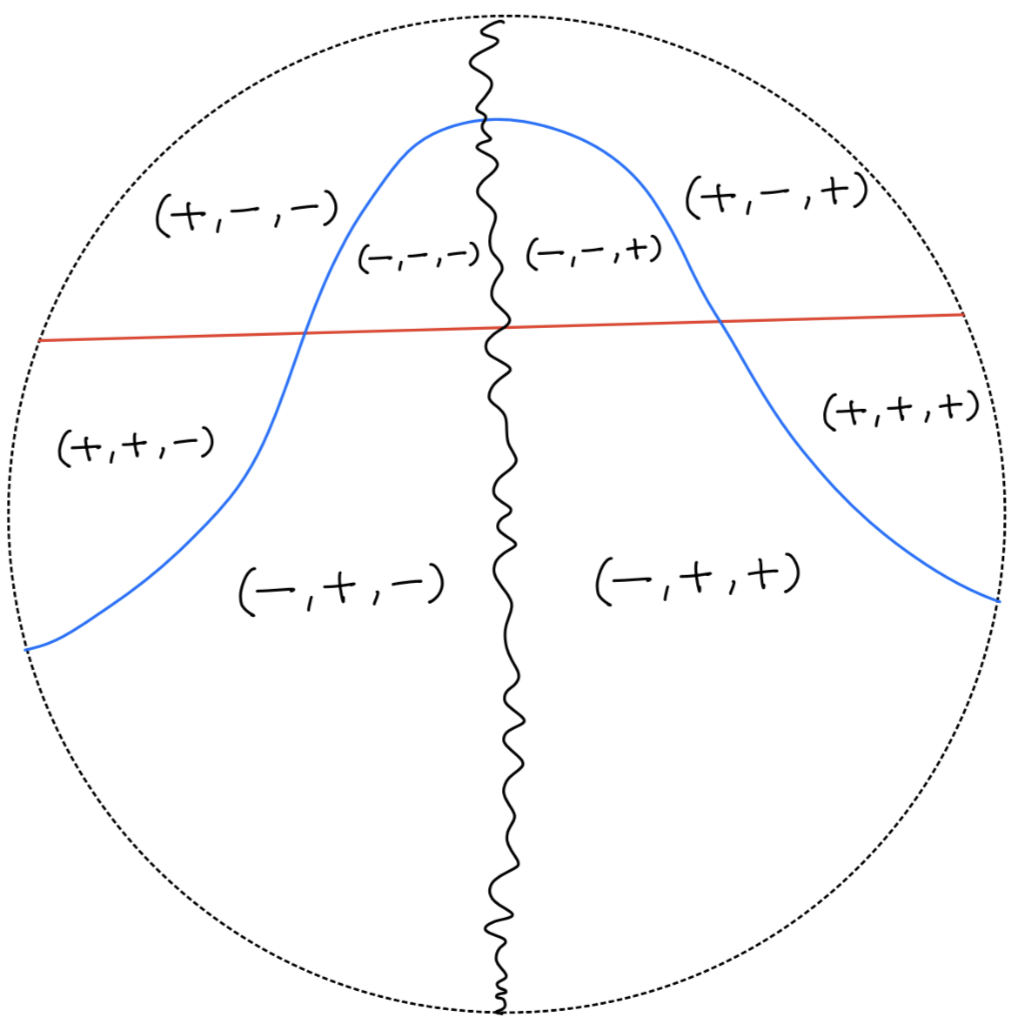
\includegraphics[width=\linewidth]{diagrams/lemma3/1.png} % Adjust the width as needed
    \caption{Your caption here}
    \label{fig:your-label}
\end{figure}

Stalks :\\

- 1 : $\mathbb{C}^{m+1}$\\
- 2 : $\mathbb{C}^{m}$\\
- 3 : $\mathbb{C}^{m}$\\
- 4 : $\mathbb{C}^{m+1}$\\
- 5 : $\mathbb{C}^{m+2}$\\
- 6 : $\mathbb{C}^{m+1}$\\
- 7 : $\mathbb{C}^{m+1}$\\
- 8 : $\mathbb{C}^{m+2}$\\

Generization maps : \\

- 2$\rightarrow$1 : $\iota_l$\\
- 6$\rightarrow$5 : $\iota_l$\\
- 1$\rightarrow$4 : $\iota_l$\\
- 1$\rightarrow$5 : $\iota_f$\\
- 2$\rightarrow$6 : $\iota_f$\\
- 1$\rightarrow$4 : $f$\\
- 2$\rightarrow$3 : $g$\\
- 6$\rightarrow$7 : $h$\\
- 3$\rightarrow$4 : $h'$\\
- 7$\rightarrow$8 : $g'$\\
- 3$\rightarrow$7 : $h''$\\
- 4$\rightarrow$8 : $f''$\\

\begin{figure}[H] % Optional: [h] means here, [t] for top, [b] for bottom, [p] for page of floats
    \centering
    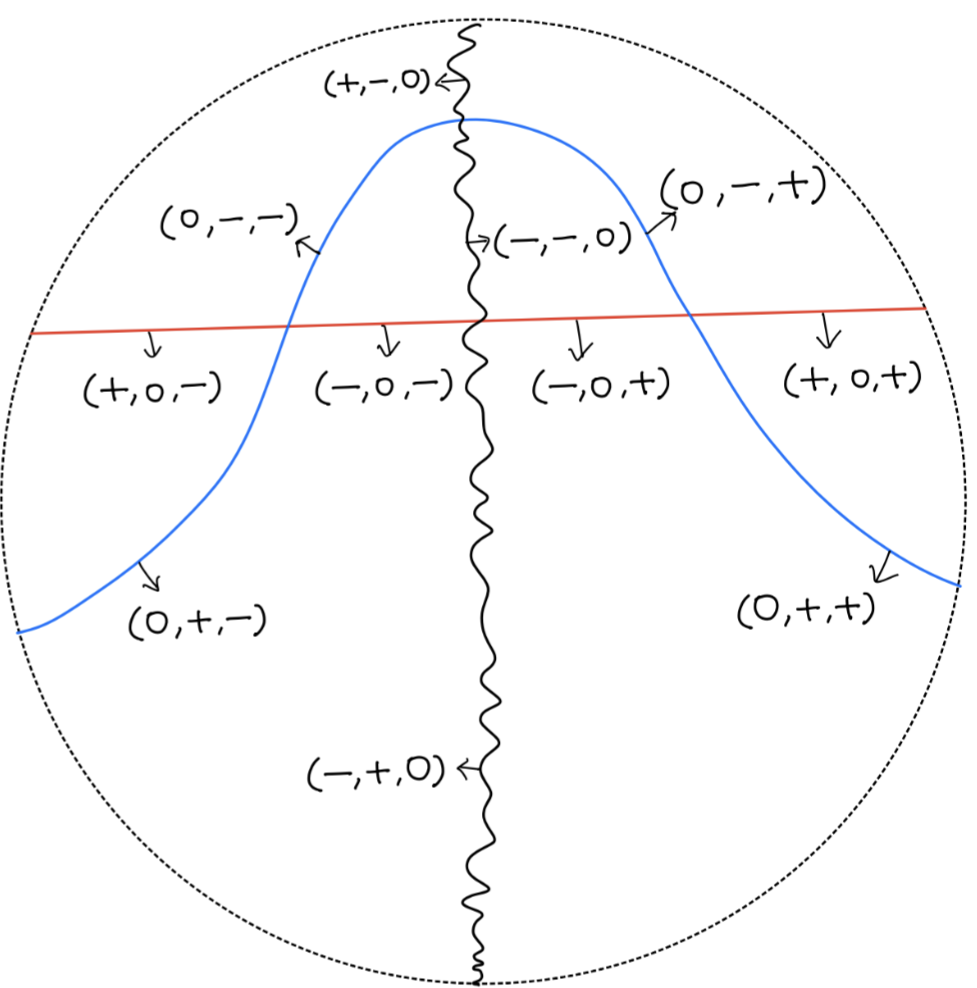
\includegraphics[width=\linewidth]{diagrams/lemma3/2.png} % Adjust the width as needed
    \caption{Your caption here}
    \label{fig:your-label}
\end{figure}

Stalks :\\

- 1 : $\mathbb{C}^{m+1}$\\
- 2 : $\mathbb{C}^{m+2}$\\
- 3 : $\mathbb{C}^{m+1}$\\
- 4 : $\mathbb{C}^{m+1}$\\
- 5 : $\mathbb{C}^{m+2}$\\
- 6 : $\mathbb{C}^{m+1}$\\

Generization maps : \\
- 1$\rightarrow$3 : $\iota_f$\\
- 2$\rightarrow$4 : $\iota_f$\\
- 5$\rightarrow$3 : $\iota_l$\\
- 6$\rightarrow$4 : $\iota_l$\\
- 1$\rightarrow$2 : $f$\\
- 5$\rightarrow$6 : $g$\\
- 2$\rightarrow$4 : $f'$\\
- 6$\rightarrow$4 : $g'$\\
- 3$\rightarrow$4 : $T$\\

where \\
- $T_{(1,1),(m+2,m+1)} = f'\circ f$\\
- $T_{(1,2),(m+2,m+2)}=g'\circ g$\\

We define an isotopy between $\mathfrak{F}$ and $\mathfrak{F}'$ called $isotopy_3$ as follows :\\

$(\Rn{1})$ The trajectory of red strand in $D\times [0,1]$ is $\{(x,y,t)\in D\times [0,1]~|~ y =\frac{1}{2}\}$\\

$(\Rn{2})$ The trajectory of blue strand in $D\times [0,1]$ is $\{(x,y,t)\in D\times [0,1]~|~ y =\frac{5}{3}(t-1)x^2 - \frac{5}{4}+\frac{3}{4}\}$. When $t=t_0$, the above set is a parabola passing through $(-\frac{\sqrt{3}}{2}, -\frac{1}{2})$, $(\frac{\sqrt{3}}{2}, -\frac{1}{2})$, $(0, -\frac{5}{4}t_0 + \frac{3}{4})$\\

$(\Rn{3})$ The trajectory of squiggly line in $D\times [0,1]$ is $\{(x,y,t)\in D\times [0,1]~|~ x =0\}$\\

Now we will describe the sheaf isotopy from $\mathfrak{F}$ to $\mathfrak{F}'$ by assigning stalks to the 8 regions separated by $(\Rn{1},\Rn{2},\Rn{3})$ and generization maps between them.\\

First let's list the 8 regions :\\

1. $\{(x,y,t)\in D\times [0,1]~|~ y \geq \frac{5}{3}(t-1)x^2 - \frac{5}{4} + \frac{3}{4}, y \geq \frac{1}{2}, x\leq 0\}$\\

2. $\{(x,y,t)\in D\times [0,1]~|~ y \geq \frac{5}{3}(t-1)x^2 - \frac{5}{4} + \frac{3}{4}, y \geq \frac{1}{2}, x\geq 0\}$\\

3. $\{(x,y,t)\in D\times [0,1]~|~ y \leq \frac{5}{3}(t-1)x^2 - \frac{5}{4} + \frac{3}{4}, y \geq \frac{1}{2}, x\leq 0\}$\\

4. $\{(x,y,t)\in D\times [0,1]~|~ y \leq \frac{5}{3}(t-1)x^2 - \frac{5}{4} + \frac{3}{4}, y \geq \frac{1}{2}, x\geq 0\}$\\

5. $\{(x,y,t)\in D\times [0,1]~|~ y \geq \frac{5}{3}(t-1)x^2 - \frac{5}{4} + \frac{3}{4}, y \leq \frac{1}{2}, x\leq 0\}$\\

6. $\{(x,y,t)\in D\times [0,1]~|~ y \geq \frac{5}{3}(t-1)x^2 - \frac{5}{4} + \frac{3}{4}, y \leq \frac{1}{2}, x\geq 0\}$

7. $\{(x,y,t)\in D\times [0,1]~|~ y \leq \frac{5}{3}(t-1)x^2 - \frac{5}{4} + \frac{3}{4}, y \leq \frac{1}{2}, x\leq 0\}$\\

8. $\{(x,y,t)\in D\times [0,1]~|~ y \leq \frac{5}{3}(t-1)x^2 - \frac{5}{4} + \frac{3}{4}, y \leq \frac{1}{2}, x\geq 0\}$

Now let's define :\\

Stalks :\\

- 1 : $\mathbb{C}^{m+1}$\\
- 2 : $\mathbb{C}^{m+1}$\\
- 3 : $\mathbb{C}^{m}$\\
- 4 : $\mathbb{C}^{m}$\\
- 5 : $\mathbb{C}^{m+2}$\\
- 6 : $\mathbb{C}^{m+2}$\\
- 7 : $\mathbb{C}^{m+1}$\\
- 8 : $\mathbb{C}^{m+1}$\\

Generization maps : \\

- 3$\rightarrow$1 : $\iota_l$\\
- 7$\rightarrow$5 : $\iota_l$\\
- 1$\rightarrow$5 : $\iota_f$\\
- 3$\rightarrow$7 : $\iota_f$\\
- 1$\rightarrow$2 : $f$\\
- 3$\rightarrow$4 : $h$\\
- 7$\rightarrow$8 : $g$\\
- 4$\rightarrow$2 : $h'$\\
- 8$\rightarrow$6 : $g'$\\
- 4$\rightarrow$8 : $h''$\\
- 2$\rightarrow$6 : $f'$\\
- 5$\rightarrow$6 : $T$\\

Below we will prove that this is a well-defined isotopy between $\mathfrak{F}$ and $\mathfrak{F}'$\\

(proof of well-definedness)
\section{lemma4(core)}

\begin{lemma}
\end{lemma}

\begin{figure}[H] % Optional: [h] means here, [t] for top, [b] for bottom, [p] for page of floats
    \centering
    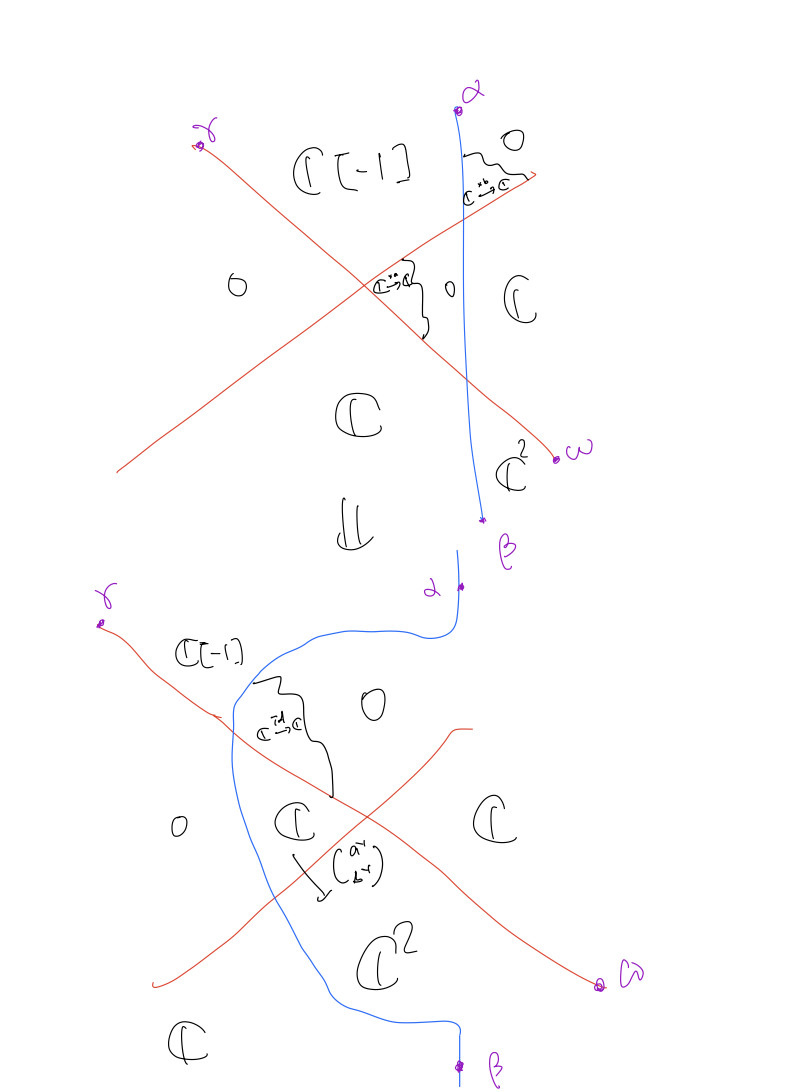
\includegraphics[width=\linewidth]{diagrams/lemma4/1.png} % Adjust the width as needed
    \caption{Your caption here}
    \label{fig:your-label}
\end{figure}
\section{definition5}
\begin{definition}
\end{definition}
Suppose we have the following local diagram:

\begin{figure}[H] % Optional: [h] means here, [t] for top, [b] for bottom, [p] for page of floats
    \centering
    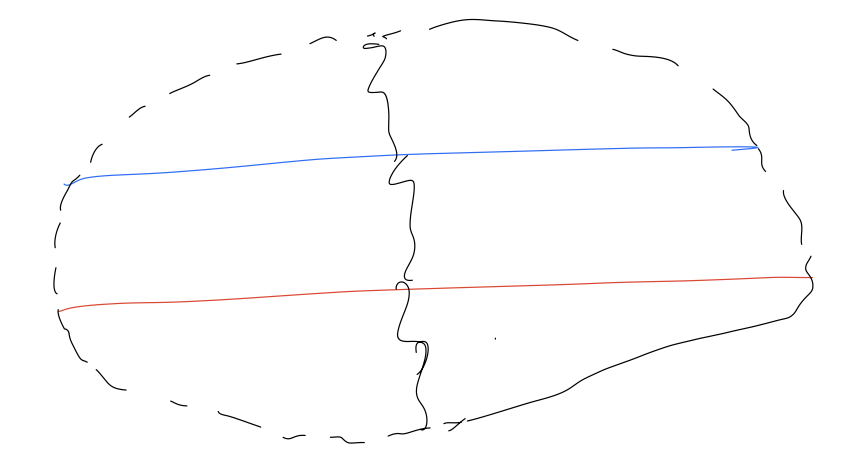
\includegraphics[width=\linewidth]{diagrams/definition5/1.png} % Adjust the width as needed
    \caption{Your caption here}
    \label{fig:your-label}
\end{figure}

Let's apply a collection of moves as follows:

(Step1) Apply MOVE \RN{1} to the regions surrounded by purple dotted lines:

\begin{figure}[H] % Optional: [h] means here, [t] for top, [b] for bottom, [p] for page of floats
    \centering
    \includegraphics[width=\linewidth]{diagrams/definition5/2.png} % Adjust the width as needed
    \caption{Your caption here}
    \label{fig:your-label}
\end{figure}

(Step2) Apply MOVE \RN{3} to the following diagram :
\begin{figure}[H] % Optional: [h] means here, [t] for top, [b] for bottom, [p] for page of floats
    \centering
    \includegraphics[width=\linewidth]{diagrams/definition5/3.png} % Adjust the width as needed
    \caption{Your caption here}
    \label{fig:your-label}
\end{figure}

We call this sequential application of moves as MOVE \RN{5}.
\section{lemma5}
\begin{lemma}
\end{lemma}
Suppose we have a Riemann sphere $C$ and a diagram $(C,\iota,\xi)$ and a regular cell complex refinement $\overline{(C,\iota,\xi)}$ and a sheaf $\mathfrak{F}$ singular supported on it such that when restricted to a small disk $D\subset C$ the refinement is as the following figure :

\begin{figure}[H] % Optional: [h] means here, [t] for top, [b] for bottom, [p] for page of floats
    \centering
    \includegraphics[width=\linewidth]{diagrams/lemma5/1.png} % Adjust the width as needed
    \caption{Your caption here}
    \label{fig:your-label}
\end{figure}

Stalks :\\

- 1 : $\mathbb{C}^{m+1}$\\
- 2 : $\mathbb{C}^{m+1}$\\
- 3 : $\mathbb{C}^{m}$\\
- 4 : $\mathbb{C}^{m}$\\
- 5 : $\mathbb{C}^{m+1}$\\
- 6 : $\mathbb{C}^{m+1}$\\


Let $T$ be a block diagonal matrix of size $(1,m,1)$. We denote the submatrix of $T$ with index range $a\leq i \leq b$,$a\leq j \leq b$ to be $T_{a,b}$. \\

Let m be arbitrary positive integer, then we denote the inclusion map from $\mathbb{C}^{m}$ to $\mathbb{C}^{m+1}$ that sends $e_i$ to $e_i$($e_{i+1}$ resp.) by $\iota_f$($\iota_l$ resp.)\\

Generization maps :\\

- 1$\rightarrow$2 : $T_{1,m+1}$\\
- 3$\rightarrow$4 : $T_{2,m+1}$\\
- 5$\rightarrow$6 : $T_{2,m+1}$\\
- 3$\rightarrow$1 : $\iota_l$\\
- 4$\rightarrow$2 : $\iota_l$\\
- 3$\rightarrow$5 : $\iota_f$\\
- 4$\rightarrow$6 : $\iota_f$\\

Now we apply a sequence of isotopies to $\mathfrak{F}$ which will be called $isotopy_5$ :\\

(step1) Inside the disk surrounded by purple circle apply $isotopy_1$

\begin{figure}[H] % Optional: [h] means here, [t] for top, [b] for bottom, [p] for page of floats
    \centering
    \includegraphics[width=\linewidth]{diagrams/lemma5/2.png} % Adjust the width as needed
    \caption{Your caption here}
    \label{fig:your-label}
\end{figure}

we get the following diagram :
\begin{figure}[H] % Optional: [h] means here, [t] for top, [b] for bottom, [p] for page of floats
    \centering
    \includegraphics[width=\linewidth]{diagrams/lemma5/3.png} % Adjust the width as needed
    \caption{Your caption here}
    \label{fig:your-label}
\end{figure}
(step2) Now apply $isotopy_3$ inside the disk surrounded by the purple circle:
\begin{figure}[H] % Optional: [h] means here, [t] for top, [b] for bottom, [p] for page of floats
    \centering
    \includegraphics[width=\linewidth]{diagrams/lemma5/4.png} % Adjust the width as needed
    \caption{Your caption here}
    \label{fig:your-label}
\end{figure}

We get the following diagram and a sheaf :

\begin{figure}[H] % Optional: [h] means here, [t] for top, [b] for bottom, [p] for page of floats
    \centering
    \includegraphics[width=\linewidth]{diagrams/lemma5/5.png} % Adjust the width as needed
    \caption{Your caption here}
    \label{fig:your-label}
\end{figure}

Stalks : \\
- 1 : $\mathbb{C}^{m}$\\
- 2 : $\mathbb{C}^{m+1}$\\
- 3 : $\mathbb{C}^{m+1}$\\
- 4 : $\mathbb{C}^{m}$\\
- 5 : $\mathbb{C}^{m+1}$\\
- 6 : $\mathbb{C}^{m+2}$\\
- 7 : $\mathbb{C}^{m+2}$\\
- 8 : $\mathbb{C}^{m+1}$\\

Generization maps : \\


- 1$\rightarrow$2 : $\iota_l$\\
- 4$\rightarrow$3 : $\iota_l$\\
- 1$\rightarrow$5 : $\iota_f$\\
- 4$\rightarrow$8 : $\iota_f$\\
- 2$\rightarrow$6 : $\iota_f$\\
- 3$\rightarrow$7 : $\iota_f$\\
- 5$\rightarrow$6 : $\iota_l$\\
- 8$\rightarrow$7 : $\iota_l$\\
- 2$\rightarrow$3 : $T_{1,m+1}$\\
- 6$\rightarrow$7 : $T_{1,m+2}$\\
- 5$\rightarrow$8 : $T_{2,m+2}$\\

(proof) After (step1), by lemma1, we get the following sheaf :
\begin{figure}[H] % Optional: [h] means here, [t] for top, [b] for bottom, [p] for page of floats
    \centering
    \includegraphics[width=\linewidth]{diagrams/lemma5/6.png} % Adjust the width as needed
    \caption{Your caption here}
    \label{fig:your-label}
\end{figure}

Stalks : \\
- 1 : $\mathbb{C}^{m}$\\
- 2 : $\mathbb{C}^{m+1}$\\
- 3 : $\mathbb{C}^{m}$\\
- 4 : $\mathbb{C}^{m}$\\
- 5 : $\mathbb{C}^{m+1}$\\
- 6 : $\mathbb{C}^{m}$\\
- 7 : $\mathbb{C}^{m+1}$\\
- 8 : $\mathbb{C}^{m+2}$\\
- 9 : $\mathbb{C}^{m+1}$\\
- 10 : $\mathbb{C}^{m+2}$\\

Generization maps : \\


- 1$\rightarrow$2 : $\iota_l$\\
- 3$\rightarrow$2 : $\iota_l$\\
- 4$\rightarrow$5 : $\iota_l$\\
- 6$\rightarrow$5 : $\iota_l$\\
- 1$\rightarrow$7 : $\iota_f$\\
- 3$\rightarrow$7 : $\iota_f$\\
- 4$\rightarrow$9 : $\iota_f$\\
- 6$\rightarrow$9 : $\iota_f$\\
- 2$\rightarrow$8 : $\iota_f$\\
- 7$\rightarrow$8 : $\iota_f$\\
- 5$\rightarrow$10 : $\iota_f$\\
- 9$\rightarrow$10 : $\iota_l$\\
- 2$\rightarrow$5 : $T_{1,m+1}$\\
- 3$\rightarrow$4 : $T_{2,m+1}$\\
- 7$\rightarrow$9 : $T_{2,m+2}$\\

Now to the above sheaf we apply (step2), then by lemma3, we get the final sheaf.
\section{definition6}
\begin{definition}
\end{definition}
Suppose we have a Riemann sphere $C$ and a diagram $(C,\iota,\xi)$ and a regular cell complex refinement $\overline{(C,\iota,\xi)}$ and a sheaf $\mathfrak{F}$ singular supported on it such that when restricted to a small disk $D\subset C$, the refinement is as following figure where 2 dimensional strata are labeled by tuples

\begin{figure}[H] % Optional: [h] means here, [t] for top, [b] for bottom, [p] for page of floats
    \centering
    \includegraphics[scale = 0.95]{diagrams/definition6/1.png} % Adjust the width as needed
    \caption{Your caption here}
    \label{fig:your-label}
\end{figure}

Stalks :\\
- $(i,0)$ : $\mathbb{C}^{m+|i|}$\\
- $(i,1)$ : $\mathbb{C}^{m+|i|}$\\

Generization maps\\
- the maps corresponding to the arrow crossing the red strand is $\iota_f$\\
- the maps corresponding to the arrow crossing the blue strand is $\iota_l$\\
- $(i,0)\rightarrow (i,1)$ where $i\geq 0$ : $\tilde{T}_{k+1-i,m+k}$\\
- $(i,0)\rightarrow (i,1)$ where $i=-1$ : $\tilde{T}_{k+1,m+k+1}$\\
\\
where $\tilde{T}_{1,m+k}$ is an isomorphism preserving the flag $\mathbb{C}^m\subset_l \mathbb{C}^{m+1}\subset_l \cdots \subset_l \mathbb{C}^{m+k}$ and $T_{k+1,m+k+2}$ is an isomorphism preserving the flag $\mathbb{C}^m \subset_f \mathbb{C}^{m+1}$.

Now we will define isotopy starting from the above sheaf $\mathfrak{F}$ inductively on the number of blue strands so that the final sheaf $\mathfrak{F}'$ is
\begin{figure}[H] % Optional: [h] means here, [t] for top, [b] for bottom, [p] for page of floats
    \centering
    \includegraphics[scale = 0.95]{diagrams/definition6/2.png} % Adjust the width as needed
    \caption{Your caption here}
    \label{fig:your-label}
\end{figure}

In the above diagram, I have intentionally omitted lines connecting
- $\alpha_i$ and $\beta_i$
- $\alpha'_i$ and $\beta'_i$
for $i=1,\cdots,k$ so as not to make diagram too messy. These omitted lines are mutually disjoint and crosses red strand only once.
Let the crossing of the red strand with $\overline{\alpha_i \beta_i}$ be called $c_i$ and $\overline{\alpha'_i \beta'_i}$ be called $c'_i$.
Let's denote the north, east, west, south of the crossing $c_i$($c'_i$ resp.) as $N_i,E_i,W_i,S_i$($N'_i,E'_i,W'_i,S'_i$ resp.).

The final sheaf will be described as follows:

Stalks\\
- $W_i,E'_i$ : $\mathbb{C}^{m+i}$ \\
- $N_i,N'_i$ : $\mathbb{C}^{m+i+1}$ \\
- $S_1,E_1$ : $\mathbb{C}^{m}, \mathbb{C}^{m+1}$\\
- $W'_1,S'_1$ : $\mathbb{C}^{m+1}, \mathbb{C}^m$\\

Generization maps\\ 
- maps crossing blue strands are $\iota_l$\\
- maps crossing red strands are $\iota_f$\\
- maps crossing squiggly lines are\\
	- $E_1\rightarrow W'_1$ : $T' = \tilde{T}_{k+!,m+k+1}$\\
	- $W_k\rightarrow E'_k$ : $T = \tilde{T}_{1,m+k}$\\
	- $N_i \rightarrow N'_i$ : $\tilde{T}_{k-i+1,m+k+1}$\\
	
	
when n=1, (skip this part for now)

Suppose $isotopy_6$ is defined up to the number of blue strands less than $n$. Now we define $isotopy_6$ for the number of blue strands $=n$.

(step1) Apply $isotopy_6$ for the number of blue strands $n-1$ on the disk surrounded by purple dotted line which is well-defined by the induction hypothesis.

\begin{figure}[H] % Optional: [h] means here, [t] for top, [b] for bottom, [p] for page of floats
    \centering
    \includegraphics[scale = 0.95]{diagrams/definition6/3.png} % Adjust the width as needed
    \caption{Your caption here}
    \label{fig:your-label}
\end{figure}

we get the following diagram

\begin{figure}[H] % Optional: [h] means here, [t] for top, [b] for bottom, [p] for page of floats
    \centering
    \includegraphics[scale = 0.95]{diagrams/definition6/4.png} % Adjust the width as needed
    \caption{Your caption here}
    \label{fig:your-label}
\end{figure}

(step2) Apply $isotopy_6$ for the number of blue strands $=1$ on the disk surrounded by purple dotted line

\begin{figure}[H] % Optional: [h] means here, [t] for top, [b] for bottom, [p] for page of floats
    \centering
    \includegraphics[scale = 0.95]{diagrams/definition6/5.png} % Adjust the width as needed
    \caption{Your caption here}
    \label{fig:your-label}
\end{figure}

we get the final diagram

\begin{figure}[H] % Optional: [h] means here, [t] for top, [b] for bottom, [p] for page of floats
    \centering
    \includegraphics[scale = 0.95]{diagrams/definition6/6.png} % Adjust the width as needed
    \caption{Your caption here}
    \label{fig:your-label}
\end{figure}

with sheaf $\mathfrak{F}$ on it.
(proof)
\section{lemma6}
\begin{lemma}
\end{lemma}
Suppose we have a local braid diagram and a sheaf singular supported along the braids represented by the following:

\begin{figure}[H] % Optional: [h] means here, [t] for top, [b] for bottom, [p] for page of floats
    \centering
    \includegraphics[width=\linewidth]{diagrams/lemma6/1.png} % Adjust the width as needed
    \caption{Your caption here}
    \label{fig:your-label}
\end{figure}
where $T$ is an isomorphism preserving the flag $\mathbb{C}^m\subset_l \mathbb{C}^{m+1}\subset_l\cdots\subset_l \mathbb{C}^{m+k}$(here $\subset_l$ denotes inclusion into the last factors), $T'$ is an isomorphism preserving $\mathbb{C}^m \subset_f \mathbb{C}^{m+1}$(here $\subset_f$ means inclusion into the first factors), and $T_{k+1,m+k}=T'_{1,m}$.

If we apply MOVE \RN{6} to the above diagram and the sheaf on it, we get the following:
\begin{figure}[H] % Optional: [h] means here, [t] for top, [b] for bottom, [p] for page of floats
    \centering
    \includegraphics[width=\linewidth]{diagrams/lemma6/2.png} % Adjust the width as needed
    \caption{Your caption here}
    \label{fig:your-label}
\end{figure}
where $\tilde{T}_{1,m+k} = T$ and $\tilde{T}_{k+1,m+k+1} = T'$(rest of the entries are 0)

(proof) We prove the claim by induction on $k$. By the induction hypothesis after $k-1$ application of MOVE \RN{5}(MOVE \RN{6}), we get 
\begin{figure}[H] % Optional: [h] means here, [t] for top, [b] for bottom, [p] for page of floats
    \centering
    \includegraphics[width=\linewidth]{diagrams/lemma6/3.png} % Adjust the width as needed
    \caption{Your caption here}
    \label{fig:your-label}
\end{figure}

Now we apply MOVE \RN{5} to the uppermost blue strand and the red strand, then by Lemma5, we get

\begin{figure}[H] % Optional: [h] means here, [t] for top, [b] for bottom, [p] for page of floats
    \centering
    \includegraphics[width=\linewidth]{diagrams/lemma6/4.png} % Adjust the width as needed
    \caption{Your caption here}
    \label{fig:your-label}
\end{figure}
\section{definition7}
\begin{definition}
\end{definition}

Suppose we have the following diagram of alternating $m$ red strands($R_1 - R_m$) and $m$ blue strands($B_1 - B_m$) labeled from the top:

\begin{figure}[H] % Optional: [h] means here, [t] for top, [b] for bottom, [p] for page of floats
    \centering
    \includegraphics[width=\linewidth]{diagrams/definition7/1.png} % Adjust the width as needed
    \caption{Your caption here}
    \label{fig:your-label}
\end{figure}

We define MOVE \RN{7}-(a) inductively so that the final diagram looks as follows:

\begin{figure}[H] % Optional: [h] means here, [t] for top, [b] for bottom, [p] for page of floats
    \centering
    \includegraphics[width=\linewidth]{diagrams/definition7/2.png} % Adjust the width as needed
    \caption{Your caption here}
    \label{fig:your-label}
\end{figure}

We define MOVE \RN{7}-(a) inductively on $m$.
If $m=1$, then MOVE\RN{7}-(a) is the null move. If $m>1$,
(Step1) Apply MOVE\RN{7}-(a) to the first $m-1$ blue and red strands($B_1 - B_{m-1}$ and $R_1 - R_{m-1}$)(this has been defined by the induction hypothesis), we get :

\begin{figure}[H] % Optional: [h] means here, [t] for top, [b] for bottom, [p] for page of floats
    \centering
    \includegraphics[width=\linewidth]{diagrams/definition7/3.png} % Adjust the width as needed
    \caption{Your caption here}
    \label{fig:your-label}
\end{figure}

(Step2) Apply MOVE \RN{6} to $B_1 - B_{m-1}$ and $R_m$, we get :
\begin{figure}[H] % Optional: [h] means here, [t] for top, [b] for bottom, [p] for page of floats
    \centering
    \includegraphics[width=\linewidth]{diagrams/definition7/4.png} % Adjust the width as needed
    \caption{Your caption here}
    \label{fig:your-label}
\end{figure}
By induction, we have defined MOVE \RN{7}-(a) for all $m\in \mathbb{M}$.

(b) Suppose we have the following diagram of $n$ red strands($R_1 - R_n$) and $m$ blue strands($B_1 - B_m$) labeled from the top :
\begin{figure}[H] % Optional: [h] means here, [t] for top, [b] for bottom, [p] for page of floats
    \centering
    \includegraphics[width=\linewidth]{diagrams/definition7/5.png} % Adjust the width as needed
    \caption{Your caption here}
    \label{fig:your-label}
\end{figure}

We define MOVE \RN{7}-(b) inductively so that the final diagram looks as follows:
\begin{figure}[H] % Optional: [h] means here, [t] for top, [b] for bottom, [p] for page of floats
    \centering
    \includegraphics[width=\linewidth]{diagrams/definition7/6.png} % Adjust the width as needed
    \caption{Your caption here}
    \label{fig:your-label}
\end{figure}

We define MOVE \RN{7}-(b) inductively on $n$. If $n=1$, then MOVE \RN{7}-(b) is MOVE \RN{6}. If $n>1$, 
(Step1) apply MOVE \RN{7}-(b) to the first $m$ blue strands($B_1 - B_m$) and $n-1$ red strands($R_1 - R_{n-1}$)(this has been defined by the induction hypothesis), we get :
\begin{figure}[H] % Optional: [h] means here, [t] for top, [b] for bottom, [p] for page of floats
    \centering
    \includegraphics[width=\linewidth]{diagrams/definition7/7.png} % Adjust the width as needed
    \caption{Your caption here}
    \label{fig:your-label}
\end{figure}

(step2) apply MOVE \RN{6} to be $B_1 - B_m$ and $R_n$, we get the final diagram :
\begin{figure}[H] % Optional: [h] means here, [t] for top, [b] for bottom, [p] for page of floats
    \centering
    \includegraphics[width=\linewidth]{diagrams/definition7/8.png} % Adjust the width as needed
    \caption{Your caption here}
    \label{fig:your-label}
\end{figure}

By induction, we have defined MOVE \RN{7}-(b) for all $m\in \mathbb{N}$.
\section{lemma7}
\begin{lemma}
\end{lemma}

Suppose we have a Riemann sphere $C$ and a diagram $(C,\iota, \xi)$ and a regular cell complex refinement $\overline{(C,\iota, \xi)}$ and a sheaf $\mathfrak{F}$ singular supported on it such that when restricted to a small disk $D\subset C$, the refinement is a the following figure where two dimensional strata are labeld by tuples.

\begin{figure}[H] % Optional: [h] means here, [t] for top, [b] for bottom, [p] for page of floats
    \centering
    \includegraphics[width=\linewidth]{diagrams/lemma7/1.png} % Adjust the width as needed
    \caption{Your caption here}
    \label{fig:your-label}
\end{figure}

Stalks : \\
$(i,0)$ : $0$\\
$(i,1),(i,2))$ : $\mathbb{C}$\\

Generization maps :\\
$(i,1)\rightarrow (i,2)$ :  multiplication by $a_i \in \mathbb{C}$\\
All the other maps are zero maps.\\

Now we will define isotopy starting from the above sheaf $\mathfrak{F}$ inductively on the number of blue strands(=the number of red strands) so that the final sheaf $\mathfrak{F}'$ is :

\begin{figure}[H] % Optional: [h] means here, [t] for top, [b] for bottom, [p] for page of floats
    \centering
    \includegraphics[width=\linewidth]{diagrams/lemma7/2.png} % Adjust the width as needed
    \caption{Your caption here}
    \label{fig:your-label}
\end{figure}


In the above diagram, I have intentionally omitted lines connecting \\
- $\alpha_i$ and $\beta_i$ for $i=1,\cdots,m$\\
- $\alpha'_i$ and $\beta'_i$ for $i=1,\cdots,m$\\
so as not to make diagram too messy. These omitted lines are mutually disjoint and crosses each red strand at most once. Let the crossing of $\overline{\alpha_j \beta_j}$ with the $i^th$ red strand be called $c_{i,j}$ and $\overline{\alpha'_j \beta'_j}$ with the $i^th$ red strand be called $c'_{i,j}$.\\
Let's denote the north, east, west, south of the crossing $c_{i,j}$($c_{i,j}$ resp.) as $N_i,E_i,W_i,S_i$($N'_i,E'_i,W'_i,S'_i$).\\

\bigskip

The final sheaf will be described as follows :\\

Stalks :\\
for $i>j$,\\
- $E_{i,j}$ : $\mathbb{C}^{i-j}$\\
- $S_{i,j}$ : $\mathbb{C}^{i-j-1}$\\
- $W_{i,j}$ : $\mathbb{C}^{i-j}$\\
- $N_{i,j}$ : $\mathbb{C}^{i-j+1}$\\
\\
- $E'_{i,j}$ : $\mathbb{C}^{i-j}$\\
- $S'_{i,j}$ : $\mathbb{C}^{i-j-1}$\\
- $W'_{i,j}$ : $\mathbb{C}^{i-j}$\\
- $N'_{i,j}$ : $\mathbb{C}^{i-j+1}$\\
\\
Generization maps : \\
- maps crossing the blue strands are $\iota_l$.\\
- maps crossing the red strands are $\iota_f$.\\
- maps crossing the squiggly lines :\\
	- for $i\geq 2$, $W_{i,1}\rightarrow E'_{i,1}$ : $T_{1,i-1}$\\
	- $N_{m,1}\rightarrow N'_{m,1}$ : $T_{1,m}$\\
	- $E_{m,j}\rightarrow W'_{m,j}$ : $T_{j+1,m}$\\
	where $T = diag(a_1,\cdots,a_m)$\\
	
Now let's define an isotopy from $\mathfrak{F}$ to $\mathfrak{F}'$ which we call$isotopy_7$.\\
If $n=1$, $isotopy_7$ is a null move.\\
Suppose we have defined $isotopy_7$ upto the number of blue strands(= the number of red strands) less than $m$. Now we define $isotopy_7$ for the number of blue strands(= the number of red strands) equals $m$ :\\

(step1) Apply $isotopy_7$ for the number of blue strands(= the number of red strands) equals $m-1$ on the disk surrounded by purple dotted line which is well-defined by the induction hypothesis.

\begin{figure}[H] % Optional: [h] means here, [t] for top, [b] for bottom, [p] for page of floats
    \centering
    \includegraphics[width=\linewidth]{diagrams/lemma7/3.png} % Adjust the width as needed
    \caption{Your caption here}
    \label{fig:your-label}
\end{figure}

We get the following diagram :

\begin{figure}[H] % Optional: [h] means here, [t] for top, [b] for bottom, [p] for page of floats
    \centering
    \includegraphics[width=\linewidth]{diagrams/lemma7/4.png} % Adjust the width as needed
    \caption{Your caption here}
    \label{fig:your-label}
\end{figure}
    
(step2) Apply $isotopy_6$ on the disk surrounded by purple dotted line.   

\begin{figure}[H] % Optional: [h] means here, [t] for top, [b] for bottom, [p] for page of floats
    \centering
    \includegraphics[width=\linewidth]{diagrams/lemma7/5.png} % Adjust the width as needed
    \caption{Your caption here}
    \label{fig:your-label}
\end{figure}

we get the final diagram :

\begin{figure}[H] % Optional: [h] means here, [t] for top, [b] for bottom, [p] for page of floats
    \centering
    \includegraphics[width=\linewidth]{diagrams/lemma7/6.png} % Adjust the width as needed
    \caption{Your caption here}
    \label{fig:your-label}
\end{figure}
\section{definition8}
\begin{definition}
\end{definition}

Suppose we have the following diagram of 2 red strands($R_1,R$) and a blue strand $B$.

\begin{figure}[H] % Optional: [h] means here, [t] for top, [b] for bottom, [p] for page of floats
    \centering
    \includegraphics[width=\linewidth]{diagrams/definition8/1.png} % Adjust the width as needed
    \caption{Your caption here}
    \label{fig:your-label}
\end{figure}

We define MOVE \RN{8} as follows :

(Step1) First, apply MOVE \RN{2} to $R_1$ and $B$, then we get the following diagram :

\begin{figure}[H] % Optional: [h] means here, [t] for top, [b] for bottom, [p] for page of floats
    \centering
    \includegraphics[width=\linewidth]{diagrams/definition8/2.png} % Adjust the width as needed
    \caption{Your caption here}
    \label{fig:your-label}
\end{figure}

(Step2) Apply MOVE \RN{5}(=MOVE \RN{2}??) to $R_2$ and $B$, then we get the final diagram :

\begin{figure}[H] % Optional: [h] means here, [t] for top, [b] for bottom, [p] for page of floats
    \centering
    \includegraphics[width=\linewidth]{diagrams/definition8/3.png} % Adjust the width as needed
    \caption{Your caption here}
    \label{fig:your-label}
\end{figure}
\section{lemma8}
\begin{lemma}
\end{lemma}

Suppose we have a Riemann sphere $C$ and a diagram $(C,\iota,\xi)$ and a regular cell complex refinement $\overline{(C,\iota,\xi)}$ and a sheaf $\mathfrak{F}$ singular supported on it such that when restricted to a small disk $D\subset C$, the refinement is as the following figure where two dimensional strata are labeled :

\begin{figure}[H] % Optional: [h] means here, [t] for top, [b] for bottom, [p] for page of floats
    \centering
    \includegraphics[width=\linewidth]{diagrams/lemma8/1.png} % Adjust the width as needed
    \caption{Your caption here}
    \label{fig:your-label}
\end{figure}

Stalks :\\
- 1 : $0$
- 2 : $\mathbb{C}\xrightarrow{\times a}\mathbb{C}$\\
- 3 : $\mathbb{C}[-1]$\\
- 4 : $\mathbb{C}\xrightarrow{\times b}\mathbb{C}$\\
- 5 : $\mathbb{C}$\\
- 6 : $0$\\
- 7 : $\mathbb{C}$\\
- 8 : $\mathbb{C}^2$\\
- 9 : $\mathbb{C}$\\
- 10 : $\mathbb{C}^2$\\

Generization maps :\\
I won't write down the zero maps.\\
- 3$\rightarrow$2 : 
\begin{tikzcd}
\mathbb{C} \arrow[r,"id"]     & \mathbb{C}  \\
0 \arrow[r,]\arrow[u,] & \mathbb{C} \arrow[u,"\times a"]
\end{tikzcd}
\\
- 3$\rightarrow$4 : 
\begin{tikzcd}
\mathbb{C} \arrow[r,"id"]     & \mathbb{C}  \\
0 \arrow[r,]\arrow[u,] & \mathbb{C} \arrow[u,"\times b"]
\end{tikzcd}
\\
- 2$\rightarrow$5 : 
\begin{tikzcd}
\mathbb{C} \arrow[r,]     & 0  \\
\mathbb{C} \arrow[r,"id"]\arrow[u,"\times a"] & \mathbb{C} \arrow[u,]
\end{tikzcd}
\\
- 4$\rightarrow$7 : 
\begin{tikzcd}
\mathbb{C} \arrow[r,]     & 0  \\
\mathbb{C} \arrow[r,"id"]\arrow[u,"\times b"] & \mathbb{C} \arrow[u,]
\end{tikzcd}
\\

- 5$\rightarrow$8 : $\iota_f$\\
- 9$\rightarrow$8 ,9$\rightarrow$10 : $\iota_l$\\
- 7$\rightarrow$10 : $\mathbb{C}\rightarrow \mathbb{C}^2$ where $1\mapsto (x,y)^T$ where $x\neq 0$\\

Now we will define isotopy starting from $\mathfrak{F}$ to the final sheaf $\mathfrak{F}'$ which is described as follows:\\

\begin{figure}[H] % Optional: [h] means here, [t] for top, [b] for bottom, [p] for page of floats
    \centering
    \includegraphics[width=\linewidth]{diagrams/lemma8/2.png} % Adjust the width as needed
    \caption{Your caption here}
    \label{fig:your-label}
\end{figure}

Stalks : \\
- 1: $0$\\
- 2 : $\mathbb{C}\xrightarrow{\times a}\mathbb{C}$\\
- 3 : $\mathbb{C}\xrightarrow{\times b}\mathbb{C}$\\
- 4 : $\mathbb{C}$\\
- 5 : $\mathbb{C}$\\
- 6 : $\mathbb{C}$\\
- 7 : $\mathbb{C}$\\
- 8 : $\mathbb{C}$\\

Generization maps : \\
- 4$\rightarrow$5 : muliplication by $ab^{-1}$\\
- 4$\rightarrow$6 : $\iota_f$\\
- 5$\rightarrow$7 : $\mathbb{C}\rightarrow \mathbb{C}^2$ where $1\mapsto (z,y)^T$\\
- 6$\rightarrow$7 : $\mathbb{C}^2\rightarrow \mathbb{C}^2$ where $e_1 \mapsto (ab^{-1}x,ab^{-1}y)^T$ and $e_2 \mapsto e_2$\\
-8$\rightarrow$6, 8$\rightarrow$7 : $\iota_l$\\

Now we define $isotopy_8$ as follows :\\
(step1) Apply $isotopy_2$ inside the disk surrounded by the purple dotted line :
\begin{figure}[H] % Optional: [h] means here, [t] for top, [b] for bottom, [p] for page of floats
    \centering
    \includegraphics[width=\linewidth]{diagrams/lemma8/3.png} % Adjust the width as needed
    \caption{Your caption here}
    \label{fig:your-label}
\end{figure}

We get the following diagram :

\begin{figure}[H] % Optional: [h] means here, [t] for top, [b] for bottom, [p] for page of floats
    \centering
    \includegraphics[width=\linewidth]{diagrams/lemma8/4.png} % Adjust the width as needed
    \caption{Your caption here}
    \label{fig:your-label}
\end{figure}

(step2) Apply $isotopy_5$ on the disk surrounded by the purple dotted line:
\begin{figure}[H] % Optional: [h] means here, [t] for top, [b] for bottom, [p] for page of floats
    \centering
    \includegraphics[width=\linewidth]{diagrams/lemma8/5.png} % Adjust the width as needed
    \caption{Your caption here}
    \label{fig:your-label}
\end{figure}

We get the final diagram :

\begin{figure}[H] % Optional: [h] means here, [t] for top, [b] for bottom, [p] for page of floats
    \centering
    \includegraphics[width=\linewidth]{diagrams/lemma8/2.png} % Adjust the width as needed
    \caption{Your caption here}
    \label{fig:your-label}
\end{figure}

with sheaf $\mathfrak{F}'$ on it.\\
(proof)
\section{definition9}
\begin{definition}
\end{definition}

Suppose we have the following diagram of $2$ red strands($R_1,R_2$) and a blude strand $B$.

\begin{figure}[H] % Optional: [h] means here, [t] for top, [b] for bottom, [p] for page of floats
    \centering
    \includegraphics[width=\linewidth]{diagrams/definition9/1.png} % Adjust the width as needed
    \caption{Your caption here}
    \label{fig:your-label}
\end{figure}

We define MOVE \RN{9} as follows :

(Step1) Apply MOVE \RN{1} to pairs $(R_1,B)$ and $(R_2,B)$, we get :

\begin{figure}[H] % Optional: [h] means here, [t] for top, [b] for bottom, [p] for page of floats
    \centering
    \includegraphics[width=\linewidth]{diagrams/definition9/2.png} % Adjust the width as needed
    \caption{Your caption here}
    \label{fig:your-label}
\end{figure}

(Step2) Apply MOVE \RN{4} locally inside the region surrounded by purple dotted circle, we get :

\begin{figure}[H] % Optional: [h] means here, [t] for top, [b] for bottom, [p] for page of floats
    \centering
    \includegraphics[width=\linewidth]{diagrams/definition9/3.png} % Adjust the width as needed
    \caption{Your caption here}
    \label{fig:your-label}
\end{figure}

(Step3) Apply MOVE \RN{3} locally inside the region surrounded by purple dotted line, we get :
\begin{figure}[H] % Optional: [h] means here, [t] for top, [b] for bottom, [p] for page of floats
    \centering
    \includegraphics[width=\linewidth]{diagrams/definition9/4.png} % Adjust the width as needed
    \caption{Your caption here}
    \label{fig:your-label}
\end{figure}
\section{lemma9}
\begin{lemma}
\end{lemma}

Suppose we have a Riemann sphere $C$ and a diagram $(C,\iota,\xi)$ and a regular cell complex refinement $\overline{(C,\iota,\xi)}$ and a sheaf $\mathfrak{F}$ singular supported on it such that when restricted to a small disk $D\subset C$ the refinement is as the following figure where two dimensional strata are labeled :


\begin{figure}[H] % Optional: [h] means here, [t] for top, [b] for bottom, [p] for page of floats
    \centering
    \includegraphics[scale=0.95]{diagrams/lemma9/1.png} % Adjust the width as needed
    \caption{Your caption here}
    \label{fig:your-label}
\end{figure}

Stalks :\\

- 1 : $0$\\
- 2 : $\mathbb{C}\xrightarrow{\times a}\mathbb{C}$\\
- 3 : $\mathbb{C}[-1]$\\
- 4 : $\mathbb{C}\xrightarrow{\times b}\mathbb{C}$\\
- 5 : $\mathbb{C}$\\
- 6 : $0$\\
- 7 : $\mathbb{C}\xrightarrow{\times c}\mathbb{C}$\\
- 8 : $0$\\
- 9 : $\mathbb{C}$\\
- 10 : $\mathbb{C}$\\
- 11 : $\mathbb{C}$\\

Generization maps : \\

I won't write down the zero maps.\\
- 2$\rightarrow$5 : 
\begin{tikzcd}
\mathbb{C} \arrow[r,]     & 0  \\
\mathbb{C} \arrow[r,"id"]\arrow[u,"\times a"] & \mathbb{C} \arrow[u,]
\end{tikzcd}
\\
- 3$\rightarrow$2 : 
\begin{tikzcd}
\mathbb{C} \arrow[r,"id"]     & \mathbb{C}  \\
0 \arrow[r,]\arrow[u,] & \mathbb{C} \arrow[u,"\times a"]
\end{tikzcd}
\\
- 3$\rightarrow$4 : 
\begin{tikzcd}
\mathbb{C} \arrow[r,"id"]     & \mathbb{C}  \\
0 \arrow[r,]\arrow[u,] & \mathbb{C} \arrow[u,"\times b"]
\end{tikzcd}
\\
- 4$\rightarrow$9 : 
\begin{tikzcd}
\mathbb{C} \arrow[r,]     & 0  \\
\mathbb{C} \arrow[r,"id"]\arrow[u,"\times b"] & \mathbb{C} \arrow[u,]
\end{tikzcd}
\\
- 3$\rightarrow$7 : 
\begin{tikzcd}
\mathbb{C} \arrow[r,"id"]     & \mathbb{C}  \\
0 \arrow[r,]\arrow[u,] & \mathbb{C} \arrow[u,"\times c"]
\end{tikzcd}
\\
- 7$\rightarrow$11 : 
\begin{tikzcd}
\mathbb{C} \arrow[r,]     & 0  \\
\mathbb{C} \arrow[r,"id"]\arrow[u,"\times c"] & \mathbb{C} \arrow[u,]
\end{tikzcd}
\\
- 10$\rightarrow$11 : $\mathbb{C}\xrightarrow{\times d}\mathbb{C}$\\

Now we will define isotopy starting from the above sheaf $\mathfrak{F}$ to the final sheaf $\mathfrak{F}'$. This will be called $isotopy_9$. The following figure is the sheaf $\mathfrak{F}'$ restricted to $D\subset C$.

\begin{figure}[H] % Optional: [h] means here, [t] for top, [b] for bottom, [p] for page of floats
    \centering
    \includegraphics[scale=0.95]{diagrams/lemma9/2.png} % Adjust the width as needed
    \caption{Your caption here}
    \label{fig:your-label}
\end{figure}

Stalks : \\
- 1 : $0$\\
- 2 : $\mathfrak{C}$\\
- 3 : $\mathfrak{C}$\\
- 4 : $0$\\
- 5 : $0$\\
- 6 : $\mathfrak{C}$\\
- 7 : $\mathfrak{C}^2$\\
- 8 : $\mathfrak{C}^2$\\
- 9 : $\mathfrak{C}$\\


Generization maps :\\
-7$\rightarrow$8 : $\mathbb{C}^2\rightarrow \mathbb{C}^2$ where $e_1 \mapsto (ac^{-1},ab^{-1})^T$ and $e_2\mapsto (0,d)^T$\\
- 6 $\rightarrow$9 : $\mathbb{C}\xrightarrow{\times d}\mathbb{C}$\\
- 2 $\rightarrow$ : $\mathbb{C}\rightarrow \mathbb{C}^2$ where $e_1 \mapsto (aC^{-1},ab^{-1})^T$\\
- rest of the maps crossing red strands are $\iota_f$\\
- rest of the maps crossing blue strands are $\iota_f$\\

We define $isotopy_9$ as follows :\\
(step1) Apply $isotopy_1$ inside the disk surrounded by the purple dotted lines:
\begin{figure}[H] % Optional: [h] means here, [t] for top, [b] for bottom, [p] for page of floats
    \centering
    \includegraphics[scale=0.95]{diagrams/lemma9/3.png} % Adjust the width as needed
    \caption{Your caption here}
    \label{fig:your-label}
\end{figure}
We get the following diagram :
\begin{figure}[H] % Optional: [h] means here, [t] for top, [b] for bottom, [p] for page of floats
    \centering
    \includegraphics[scale=0.95]{diagrams/lemma9/4.png} % Adjust the width as needed
    \caption{Your caption here}
    \label{fig:your-label}
\end{figure}

(step2) Apply $isotopy_4$ on the disk surrounded by purple dotted line:
\begin{figure}[H] % Optional: [h] means here, [t] for top, [b] for bottom, [p] for page of floats
    \centering
    \includegraphics[scale=0.95]{diagrams/lemma9/5.png} % Adjust the width as needed
    \caption{Your caption here}
    \label{fig:your-label}
\end{figure}

We get the following diagram :
\begin{figure}[H] % Optional: [h] means here, [t] for top, [b] for bottom, [p] for page of floats
    \centering
    \includegraphics[scale=0.95]{diagrams/lemma9/6.png} % Adjust the width as needed
    \caption{Your caption here}
    \label{fig:your-label}
\end{figure}

(step3) Apply $isotopy_8$ on the disk surrounded by purple dotted line:
\begin{figure}[H] % Optional: [h] means here, [t] for top, [b] for bottom, [p] for page of floats
    \centering
    \includegraphics[scale=0.95]{diagrams/lemma9/7.png} % Adjust the width as needed
    \caption{Your caption here}
    \label{fig:your-label}
\end{figure}

we get the following diagram :
\begin{figure}[H] % Optional: [h] means here, [t] for top, [b] for bottom, [p] for page of floats
    \centering
    \includegraphics[scale=0.95]{diagrams/lemma9/8.png} % Adjust the width as needed
    \caption{Your caption here}
    \label{fig:your-label}
\end{figure}

(step4) we can change the basis of the stalk at the region marked with purple star so that the generization map corresponding to the squiggly line next to the purple star is the identity map:

\begin{figure}[H] % Optional: [h] means here, [t] for top, [b] for bottom, [p] for page of floats
    \centering
    \includegraphics[scale=0.95]{diagrams/lemma9/9.png} % Adjust the width as needed
    \caption{Your caption here}
    \label{fig:your-label}
\end{figure}

Now the sheaf could be thought of as a sheaf singular supported on the below diagram:
\begin{figure}[H] % Optional: [h] means here, [t] for top, [b] for bottom, [p] for page of floats
    \centering
    \includegraphics[scale=0.95]{diagrams/lemma9/10.png} % Adjust the width as needed
    \caption{Your caption here}
    \label{fig:your-label}
\end{figure}

and that sheaf is $\mathfrak{F}'$.\\
(proof) By Lemma1, after (step1) we get the following sheaf
\section{definition10}
\begin{definition}
\end{definition}


Suppose we have the following diagram :

\begin{figure}[H] % Optional: [h] means here, [t] for top, [b] for bottom, [p] for page of floats
    \centering
    \includegraphics[width=\linewidth]{diagrams/definition10/1.png} % Adjust the width as needed
    \caption{Your caption here}
    \label{fig:your-label}
\end{figure}

We define MOVE \RN{10} as follows :

(Step1) Apply MOVE \RN{1} to the region inside of the purple circle :

\begin{figure}[H] % Optional: [h] means here, [t] for top, [b] for bottom, [p] for page of floats
    \centering
    \includegraphics[width=\linewidth]{diagrams/definition10/2.png} % Adjust the width as needed
    \caption{Your caption here}
    \label{fig:your-label}
\end{figure}

we get :

\begin{figure}[H] % Optional: [h] means here, [t] for top, [b] for bottom, [p] for page of floats
    \centering
    \includegraphics[width=\linewidth]{diagrams/definition10/3.png} % Adjust the width as needed
    \caption{Your caption here}
    \label{fig:your-label}
\end{figure}

(Step2) Apply MOVE \RN{1} to the region inside the purple circle :

\begin{figure}[H] % Optional: [h] means here, [t] for top, [b] for bottom, [p] for page of floats
    \centering
    \includegraphics[width=\linewidth]{diagrams/definition10/4.png} % Adjust the width as needed
    \caption{Your caption here}
    \label{fig:your-label}
\end{figure}

we get :

\begin{figure}[H] % Optional: [h] means here, [t] for top, [b] for bottom, [p] for page of floats
    \centering
    \includegraphics[width=\linewidth]{diagrams/definition10/5.png} % Adjust the width as needed
    \caption{Your caption here}
    \label{fig:your-label}
\end{figure}

(Step3) Apply MOVE \RN{4} to the region inside the purple circle :

\begin{figure}[H] % Optional: [h] means here, [t] for top, [b] for bottom, [p] for page of floats
    \centering
    \includegraphics[width=\linewidth]{diagrams/definition10/6.png} % Adjust the width as needed
    \caption{Your caption here}
    \label{fig:your-label}
\end{figure}

we get :

\begin{figure}[H] % Optional: [h] means here, [t] for top, [b] for bottom, [p] for page of floats
    \centering
    \includegraphics[width=\linewidth]{diagrams/definition10/7.png} % Adjust the width as needed
    \caption{Your caption here}
    \label{fig:your-label}
\end{figure}

(Step4) Apply MOVE \RN{3} to the region inside the purple circle :

\begin{figure}[H] % Optional: [h] means here, [t] for top, [b] for bottom, [p] for page of floats
    \centering
    \includegraphics[width=\linewidth]{diagrams/definition10/8.png} % Adjust the width as needed
    \caption{Your caption here}
    \label{fig:your-label}
\end{figure}

we get :

\begin{figure}[H] % Optional: [h] means here, [t] for top, [b] for bottom, [p] for page of floats
    \centering
    \includegraphics[width=\linewidth]{diagrams/definition10/9.png} % Adjust the width as needed
    \caption{Your caption here}
    \label{fig:your-label}
\end{figure}

(Step5) Apply MOVE \RN{5} to the region inside the purple circle :

\begin{figure}[H] % Optional: [h] means here, [t] for top, [b] for bottom, [p] for page of floats
    \centering
    \includegraphics[width=\linewidth]{diagrams/definition10/10.png} % Adjust the width as needed
    \caption{Your caption here}
    \label{fig:your-label}
\end{figure}

we get the final diagram :

\begin{figure}[H] % Optional: [h] means here, [t] for top, [b] for bottom, [p] for page of floats
    \centering
    \includegraphics[width=\linewidth]{diagrams/definition10/11.png} % Adjust the width as needed
    \caption{Your caption here}
    \label{fig:your-label}
\end{figure}
\section{lemma10}
\begin{lemma}
\end{lemma}

Suppose we have a Riemann sphere $C$ and a diagram $(C,\iota,\xi)$ and a regular cell complex refinement $\overline{(C,\iota,\xi)}$ and a sheaf $\mathfrak{F}$ singular supported on it such that when restricted to a small disk $D\subset C$  the refinement is as the following figure where two dimensional strata are labeled:

\begin{figure}[H] % Optional: [h] means here, [t] for top, [b] for bottom, [p] for page of floats
    \centering
    \includegraphics[scale = 0.95]{diagrams/lemma10/1.png} % Adjust the width as needed
    \caption{Your caption here}
    \label{fig:your-label}
\end{figure}


Stalks:\\
- 1 : $\mathbb{C}^{m+1}$\\
- 2 : $\mathbb{C}^{m+1}$\\
- 3 : $\mathbb{C}^{m}$\\
- 4 : $\mathbb{C}^{m}$\\
- 5 : $\mathbb{C}^{m+1}$\\
- 6 : $\mathbb{C}^{m+1}$\\
- 7 : $\mathbb{C}^{m+2}$\\
- 8 : $\mathbb{C}^{m+2}$\\

Generization maps:\\
- 1$\rightarrow$2 : $diag(d_0,\cdots, d_m)$\\
- 3$\rightarrow$4 : $diag(d_1,\cdots, d_m)$\\
\\
- 4$\rightarrow$5 : 
$
\begin{pmatrix}

		d_1^{-1} & \cdots & 0 \\ 
		\vdots & \ddots & \vdots\\
		0 & \cdots & d_m^{-1} \\

	\hline
	0 & \cdots &0
\end{pmatrix}
$\\
\\
- 5$\rightarrow$8 : 
$
\begin{pmatrix}
		\begin{matrix} 
			d_1 & \cdots & 0 \\ 
			\vdots & \ddots & \vdots\\
			0 & \cdots & d_m
		\end{matrix} & \vline &
		\begin{matrix}
			0\\
			\vdots\\
			\alpha
		\end{matrix}\\
		\hline
		\begin{matrix}
			0&\cdots&0\\
			0&\cdots&0
		\end{matrix}
		& \vline &
		\begin{matrix}
			\beta\\
			0
		\end{matrix}
\end{pmatrix}
$\\
\\
- 7$\rightarrow$8 :
$
\begin{pmatrix}
		\begin{matrix} 
			d_1 & \cdots & 0 \\ 
			\vdots & \ddots & \vdots\\
			0 & \cdots & d_m
		\end{matrix} & \vline &
		\begin{matrix}
			0&0\\
			\vdots&\vdots\\
			\alpha&0
		\end{matrix}\\
		\hline
		\begin{matrix}
			0&\cdots&0\\
			0&\cdots&0
		\end{matrix}
		& \vline &
		\begin{matrix}
			\beta&0\\
			0& d_0'
		\end{matrix}
\end{pmatrix}
$\\

Now we will define isotopy starting from the above sheaf $\mathfrak{F}$ to the final sheaf $\mathfrak{F}'$.

\begin{figure}[H] % Optional: [h] means here, [t] for top, [b] for bottom, [p] for page of floats
    \centering
    \includegraphics[scale = 0.95]{diagrams/lemma10/2.png} % Adjust the width as needed
    \caption{Your caption here}
    \label{fig:your-label}
\end{figure}

Stalks:\\
- 1 : $\mathbb{C}^{m+1}$\\
- 2 : $\mathbb{C}^{m+1}$\\
- 3 : $\mathbb{C}^{m}$\\
- 4 : $\mathbb{C}^{m}$\\
- 5 : $\mathbb{C}^{m+1}$\\
- 6 : $\mathbb{C}^{m+2}$\\
- 7 : $\mathbb{C}^{m+2}$\\
- 8 : $\mathbb{C}^{m+1}$\\
- 9 : $\mathbb{C}^{m+2}$\\
- 10 : $\mathbb{C}^{m+3}$\\
- 11 : $\mathbb{C}^{m+3}$\\
- 12 : $\mathbb{C}^{m+2}$\\

Generization maps:\\

- 1$\rightarrow$2 : $diag(d_0,\cdots, d_m)$\\
\\
- 2$\rightarrow$6 : 
$
\begin{pmatrix}

		d_0^{-1} & \cdots & 0 \\ 
		\vdots & \ddots & \vdots\\
		0 & \cdots & d_m^{-1} \\

	\hline
	0 & \cdots &0
\end{pmatrix}
$\\
\\
- 6$\rightarrow$10 : 
$
\begin{pmatrix}
		\begin{matrix} 
			d_0 & \cdots & 0 \\ 
			\vdots & \ddots & \vdots\\
			0 & \cdots & d_m
		\end{matrix} & \vline &
		\begin{matrix}
			0\\
			\vdots\\
			\alpha
		\end{matrix}\\
		\hline
		\begin{matrix}
			0&\cdots&0\\
			0&\cdots&0
		\end{matrix}
		& \vline &
		\begin{matrix}
			\beta\\
			0
		\end{matrix}
\end{pmatrix}
$\\
\\
- 10$\rightarrow$11 :
$
\begin{pmatrix}
		\begin{matrix} 
			d_0 & \cdots & 0 \\ 
			\vdots & \ddots & \vdots\\
			0 & \cdots & d_m
		\end{matrix} & \vline &
		\begin{matrix}
			0&0\\
			\vdots&\vdots\\
			\alpha&0
		\end{matrix}\\
		\hline
		\begin{matrix}
			0&\cdots&0\\
			0&\cdots&0
		\end{matrix}
		& \vline &
		\begin{matrix}
			\beta&0\\
			0& d_0'
		\end{matrix}
\end{pmatrix}
$\\
\\
- 10$\rightarrow$11 :
$
\begin{pmatrix}
		\begin{matrix} 
			d_1 & \cdots & 0 \\ 
			\vdots & \ddots & \vdots\\
			0 & \cdots & d_m
		\end{matrix} & \vline &
		\begin{matrix}
			0&0\\
			\vdots&\vdots\\
			\alpha&0
		\end{matrix}\\
		\hline
		\begin{matrix}
			0&\cdots&0\\
			0&\cdots&0
		\end{matrix}
		& \vline &
		\begin{matrix}
			\beta&0\\
			0& d_0'
		\end{matrix}
\end{pmatrix}
$\\

We define $isotopy_9$ as follows:\\
(step1)Apply $isotopy_1$ inside the disks surrounded by purple dotted lines
\begin{figure}[H] % Optional: [h] means here, [t] for top, [b] for bottom, [p] for page of floats
    \centering
    \includegraphics[scale = 0.95]{diagrams/lemma10/3.png} % Adjust the width as needed
    \caption{Your caption here}
    \label{fig:your-label}
\end{figure}

We get the following diagram

\begin{figure}[H] % Optional: [h] means here, [t] for top, [b] for bottom, [p] for page of floats
    \centering
    \includegraphics[scale = 0.95]{diagrams/lemma10/4.png} % Adjust the width as needed
    \caption{Your caption here}
    \label{fig:your-label}
\end{figure}

(step2) Apply $isotopy_1$ on the disk surrounded by purple dotted lines

\begin{figure}[H] % Optional: [h] means here, [t] for top, [b] for bottom, [p] for page of floats
    \centering
    \includegraphics[scale = 0.95]{diagrams/lemma10/5.png} % Adjust the width as needed
    \caption{Your caption here}
    \label{fig:your-label}
\end{figure}

We get the following diagram
\begin{figure}[H] % Optional: [h] means here, [t] for top, [b] for bottom, [p] for page of floats
    \centering
    \includegraphics[scale = 0.95]{diagrams/lemma10/6.png} % Adjust the width as needed
    \caption{Your caption here}
    \label{fig:your-label}
\end{figure}

(step3) Apply $isotopy_4$ on the disk surrounded by purple dotted line

\begin{figure}[H] % Optional: [h] means here, [t] for top, [b] for bottom, [p] for page of floats
    \centering
    \includegraphics[scale = 0.95]{diagrams/lemma10/7.png} % Adjust the width as needed
    \caption{Your caption here}
    \label{fig:your-label}
\end{figure}

We get the following diagram:

\begin{figure}[H] % Optional: [h] means here, [t] for top, [b] for bottom, [p] for page of floats
    \centering
    \includegraphics[scale = 0.95]{diagrams/lemma10/8.png} % Adjust the width as needed
    \caption{Your caption here}
    \label{fig:your-label}
\end{figure}

(step4) Apply $isotopy_3$ on the disk surrounded by purple dotted line

\begin{figure}[H] % Optional: [h] means here, [t] for top, [b] for bottom, [p] for page of floats
    \centering
    \includegraphics[scale = 0.95]{diagrams/lemma10/9.png} % Adjust the width as needed
    \caption{Your caption here}
    \label{fig:your-label}
\end{figure}

We get the following diagram

\begin{figure}[H] % Optional: [h] means here, [t] for top, [b] for bottom, [p] for page of floats
    \centering
    \includegraphics[scale = 0.95]{diagrams/lemma10/10.png} % Adjust the width as needed
    \caption{Your caption here}
    \label{fig:your-label}
\end{figure}

(step5) Apply $isotopy_3$ on the disk surrounded by purple dotted line 

\begin{figure}[H] % Optional: [h] means here, [t] for top, [b] for bottom, [p] for page of floats
    \centering
    \includegraphics[scale = 0.95]{diagrams/lemma10/11.png} % Adjust the width as needed
    \caption{Your caption here}
    \label{fig:your-label}
\end{figure}

We get the following diagram:

\begin{figure}[H] % Optional: [h] means here, [t] for top, [b] for bottom, [p] for page of floats
    \centering
    \includegraphics[scale = 0.95]{diagrams/lemma10/12.png} % Adjust the width as needed
    \caption{Your caption here}
    \label{fig:your-label}
\end{figure}

(step6) We can change the basis of the stalk at the region marked with purple start so that the generization map corresponding to the squiggly line next to the purple star is the identity map

\begin{figure}[H] % Optional: [h] means here, [t] for top, [b] for bottom, [p] for page of floats
    \centering
    \includegraphics[scale = 0.95]{diagrams/lemma10/13.png} % Adjust the width as needed
    \caption{Your caption here}
    \label{fig:your-label}
\end{figure}

Now the sheaf could be thought of as a sheaf singular supported on the below diagram
\begin{figure}[H] % Optional: [h] means here, [t] for top, [b] for bottom, [p] for page of floats
    \centering
    \includegraphics[scale = 0.95]{diagrams/lemma10/14.png} % Adjust the width as needed
    \caption{Your caption here}
    \label{fig:your-label}
\end{figure}

and the sheaf is $\mathfrak{F}'$.

(proof) By Lemma1, after (step1) we get the following sheaf
\begin{figure}[H] % Optional: [h] means here, [t] for top, [b] for bottom, [p] for page of floats
    \centering
    \includegraphics[scale = 0.95]{diagrams/lemma10/15.png} % Adjust the width as needed
    \caption{Your caption here}
    \label{fig:your-label}
\end{figure}

Stalks :\\
\section{definition11}
\begin{definition}
\end{definition}

Suppose we have a braid diagram as follows :

\begin{figure}[H] % Optional: [h] means here, [t] for top, [b] for bottom, [p] for page of floats
    \centering
    \includegraphics[width=\linewidth]{diagrams/definition11/1.png} % Adjust the width as needed
    \caption{Your caption here}
    \label{fig:your-label}
\end{figure}

we define MOVE \RN{11} so that the final diagram looks as follows :

\begin{figure}[H] % Optional: [h] means here, [t] for top, [b] for bottom, [p] for page of floats
    \centering
    \includegraphics[width=\linewidth]{diagrams/definition11/2.png} % Adjust the width as needed
    \caption{Your caption here}
    \label{fig:your-label}
\end{figure}

We define MOVE \RN{11} inductively as follows : If $m=1$, then MOVE \RN{11} is just MOVE \RN{10}. If $m>1$, then apply MOVE \RN{11} to $B_2 - B_m$ and $R_1, R_2$(this is well-defined by induction hypothesis), we get :

\begin{figure}[H] % Optional: [h] means here, [t] for top, [b] for bottom, [p] for page of floats
    \centering
    \includegraphics[width=\linewidth]{diagrams/definition11/3.png} % Adjust the width as needed
    \caption{Your caption here}
    \label{fig:your-label}
\end{figure}

Then apply MOVE \RN{10} to $B_1$ and $R_1,R_2$, we get the final diagram :

\begin{figure}[H] % Optional: [h] means here, [t] for top, [b] for bottom, [p] for page of floats
    \centering
    \includegraphics[width=\linewidth]{diagrams/definition11/4.png} % Adjust the width as needed
    \caption{Your caption here}
    \label{fig:your-label}
\end{figure}
\section{lemma11}
\begin{lemma}
\end{lemma}

Suppose we have a Riemann Sphere $C$ and a diagram $(C,\iota,\xi)$ and a regular cell complex refinement $\overline{(C,\iota,\xi)}$ and a sheaf $\mathfrak{F}$ singular supported on it such that when restricted to a small disk $D\subset C$ the refinement is as the following figure where two dimensional strata are labeled by tuples and numbers:

\begin{figure}[H] % Optional: [h] means here, [t] for top, [b] for bottom, [p] for page of floats
    \centering
    \includegraphics[scale=0.95]{diagrams/lemma11/1.png} % Adjust the width as needed
    \caption{Your caption here}
    \label{fig:your-label}
\end{figure}

Stalks:\\
- $(i,0),(i,1)$: $\mathbb{m+1-i}$\\
- 0 : $0$\\
- 1,2 : $\mathbb{C}$\\
- 3,4 : $\mathbb{C}^2$\\

Generization maps :\\

- $(i,0)\rightarrow (i,1)$ : $\mathbb{C}^{m-i+1}\rightarrow\mathbb{C}^{m-i+1}$, $D_{i,m}$\\
- 1$\rightarrow$4 : $\mathbb{C}\rightarrow\mathbb{C}^2$ where $e_1\mapsto (a,b)^T$\\
- 3$\rightarrow$4 : $\mathbb{C}^2 \rightarrow \mathbb{C}^2$ where $e_1\mapsto (a,b)^T$ and $e_2\mapsto (0,d)^T$\\
- all the other maps crossing the red strands are $\iota_f$\\
- all the other maps crossing the blue strands are $\iota_l$\\
- rest of the maps are zero maps\\

Now we will define isotopy starting from the above sheaf $\mathfrak{F}$ inductively on the number of blue strands so that the final sheaf $\mathfrak{F}'$ is
\begin{figure}[H] % Optional: [h] means here, [t] for top, [b] for bottom, [p] for page of floats
    \centering
    \includegraphics[scale=0.95]{diagrams/lemma11/2.png} % Adjust the width as needed
    \caption{Your caption here}
    \label{fig:your-label}
\end{figure}
In the above diagram I have intentionally omitted lines connecting \\
- $\alpha_i$ and $\beta_i$ for $i=1,\cdots ,m$\\
- $\alpha'_i$ and $\beta'_i$ for $i=1,\cdots ,m$\\

so as not to make diagram too messy. These omitted lines are mutually disjoint and crosses each red strand at most once. \\

Let the crossing of $\overline{\alpha_j \beta_j}$ with the upper(lower resp.) red strand be called $c_{0,j}$($c_{1,j}$ resp.) and $\overline{\alpha'_j \beta'_j}$ be called $c;_{0,j}$($c'_{1,j}$ resp.)\\

Let's denote the north, east, west, south of the crossing $c_{i,j}$($c'_{i,j}$ resp.) as $N_{i,j},E_{i,j},W_{i,j},S_{i,j}$($N'_{i,j},E'_{i,j},W'_{i,j},S'_{i,j}$ resp.)\\

The final sheaf will be describe as follows:\\

Stalks :\\
- $E_{i,j}$ : $\mathbb{C}^{m+1+i-j}$\\
- $S_{i,j}$ : $\mathbb{C}^{m+i-j}$\\
- $W_{i,j}$ : $\mathbb{C}^{m+1+i-j}$\\
- $N_{i,j}$ : $\mathbb{C}^{m+2+i-j}$\\

- $E'_{i,j}$ : $\mathbb{C}^{m+1+i-j}$\\
- $S'_{i,j}$ : $\mathbb{C}^{m+i-j}$\\
- $W'_{i,j}$ : $\mathbb{C}^{m+1+i-j}$\\
- $N'_{i,j}$ : $\mathbb{C}^{m+2+i-j}$\\

Generization maps:\\
- maps crossing red strands are $\iota_f$ and maps crossing blue strands are $\iota_l$ unless mentioned otherwise\\
- So I will describe the maps crossing squiggly lines, non $\iota_f,\iota_l$ maps only.\\
\\
- $E_{1,j}\rightarrow W'_{1,j}$ : 
$
\begin{pmatrix}
		\begin{matrix} 
			d_{j+1} & \cdots & 0 \\ 
			\vdots & \ddots & \vdots\\
			0 & \cdots & d_m
		\end{matrix} & \vline &
		\begin{matrix}
			0&0\\
			\vdots&\vdots\\
			0&0
		\end{matrix}\\
		\hline
		\begin{matrix}
			0&\cdots&0\\
			0&\cdots&0
		\end{matrix}
		& \vline &
		\begin{matrix}
			a&0\\
			b& d
		\end{matrix}
\end{pmatrix}
$\\

- $W_{0,1}\rightarrow E'_{0,1}$ : $D_{1,m}$\\
\\
- $N_{1,1}\rightarrow N'_{1,1}$ : 
$
\begin{pmatrix}
		\begin{matrix} 
			d_{1} & \cdots & 0 \\ 
			\vdots & \ddots & \vdots\\
			0 & \cdots & d_m
		\end{matrix} & \vline &
		\begin{matrix}
			0&0\\
			\vdots&\vdots\\
			0&0
		\end{matrix}\\
		\hline
		\begin{matrix}
			0&\cdots&0\\
			0&\cdots&0
		\end{matrix}
		& \vline &
		\begin{matrix}
			a&0\\
			b& d
		\end{matrix}
\end{pmatrix}
$\\
\\
- $W_{1,1}\rightarrow W'_{1,1}$ : 
$
\begin{pmatrix}
		\begin{matrix} 
			d_{1} & \cdots & 0 \\ 
			\vdots & \ddots & \vdots\\
			0 & \cdots & d_m
		\end{matrix} & \vline &
		\begin{matrix}
			0\\
			\vdots\\
			0
		\end{matrix}\\
		\hline
		\begin{matrix}
			0&\cdots&0\\
			0&\cdots&0
		\end{matrix}
		& \vline &
		\begin{matrix}
			a\\
			b
		\end{matrix}
\end{pmatrix}
$\\
\\
- $E'_{0,1}\rightarrow E_{0,1}$ : 
$
\begin{pmatrix}
		\begin{matrix} 
			d_{1}^{-1} & \cdots & 0 \\ 
			\vdots & \ddots & \vdots\\
			0 & \cdots & d_m^{-1}
		\end{matrix} \\
		\hline
		\begin{matrix} 
			0 & \cdots & 0 
		\end{matrix} 
\end{pmatrix}
$\\

If $m=1$, $isotopy_{11}$ is just $isotopy_{10}$.\\
Suppose we have defined $isotopy_{11}$ upto the number of blue strands less than $m$. Let's define $isotopy_{11}$ for the number of blue strands equals $m$:\\

(step1) Apply $isotopy_11$ for the number of blue strands equals $m-1$ on the disk surrounded by purple dotted line which is well-defined by induction hypothesis

\begin{figure}[H] % Optional: [h] means here, [t] for top, [b] for bottom, [p] for page of floats
    \centering
    \includegraphics[scale=0.95]{diagrams/lemma11/3.png} % Adjust the width as needed
    \caption{Your caption here}
    \label{fig:your-label}
\end{figure}

We get the following diagram:

\begin{figure}[H] % Optional: [h] means here, [t] for top, [b] for bottom, [p] for page of floats
    \centering
    \includegraphics[scale=0.95]{diagrams/lemma11/4.png} % Adjust the width as needed
    \caption{Your caption here}
    \label{fig:your-label}
\end{figure}

(step2) Apply $isotopy_{10}$ on the disk surrounded by purple dotted line:

\begin{figure}[H] % Optional: [h] means here, [t] for top, [b] for bottom, [p] for page of floats
    \centering
    \includegraphics[scale=0.95]{diagrams/lemma11/5.png} % Adjust the width as needed
    \caption{Your caption here}
    \label{fig:your-label}
\end{figure}

We get the final diagram:

\begin{figure}[H] % Optional: [h] means here, [t] for top, [b] for bottom, [p] for page of floats
    \centering
    \includegraphics[scale=0.95]{diagrams/lemma11/6.png} % Adjust the width as needed
    \caption{Your caption here}
    \label{fig:your-label}
\end{figure}

with $\mathfrak{F}'$ on it.\\
(proof)
\section{definition12(for the main theorem)}
\begin{definition}
\end{definition}

Suppose we have a braid diagram as follows :

\begin{figure}[H] % Optional: [h] means here, [t] for top, [b] for bottom, [p] for page of floats
    \centering
    \includegraphics[width=\linewidth]{diagrams/definition12/1.png} % Adjust the width as needed
    \caption{Your caption here}
    \label{fig:your-label}
\end{figure}

We define MOVE \RN{12} so that the final diagram looks as follows :

\begin{figure}[H] % Optional: [h] means here, [t] for top, [b] for bottom, [p] for page of floats
    \centering
    \includegraphics[width=\linewidth]{diagrams/definition12/2.png} % Adjust the width as needed
    \caption{Your caption here}
    \label{fig:your-label}
\end{figure}

We define MOVE \RN{12} as follows :

(Step1) Apply MOVE \RN{2} to the region inside the purple circle :

\begin{figure}[H] % Optional: [h] means here, [t] for top, [b] for bottom, [p] for page of floats
    \centering
    \includegraphics[width=\linewidth]{diagrams/definition12/3.png} % Adjust the width as needed
    \caption{Your caption here}
    \label{fig:your-label}
\end{figure}

we get :

\begin{figure}[H] % Optional: [h] means here, [t] for top, [b] for bottom, [p] for page of floats
    \centering
    \includegraphics[width=\linewidth]{diagrams/definition12/4.png} % Adjust the width as needed
    \caption{Your caption here}
    \label{fig:your-label}
\end{figure}

(Step2)get rid of the squiggly lines in the region inside the purple circles:

\begin{figure}[H] % Optional: [h] means here, [t] for top, [b] for bottom, [p] for page of floats
    \centering
    \includegraphics[width=\linewidth]{diagrams/definition12/5.png} % Adjust the width as needed
    \caption{Your caption here}
    \label{fig:your-label}
\end{figure}

we get :

\begin{figure}[H] % Optional: [h] means here, [t] for top, [b] for bottom, [p] for page of floats
    \centering
    \includegraphics[width=\linewidth]{diagrams/definition12/6.png} % Adjust the width as needed
    \caption{Your caption here}
    \label{fig:your-label}
\end{figure}
(Step3) Apply MOVE \RN{7}-(a) to the region inside the purple circles

\begin{figure}[H] % Optional: [h] means here, [t] for top, [b] for bottom, [p] for page of floats
    \centering
    \includegraphics[width=\linewidth]{diagrams/definition12/7.png} % Adjust the width as needed
    \caption{Your caption here}
    \label{fig:your-label}
\end{figure}

we get :

\begin{figure}[H] % Optional: [h] means here, [t] for top, [b] for bottom, [p] for page of floats
    \centering
    \includegraphics[width=\linewidth]{diagrams/definition12/8.png} % Adjust the width as needed
    \caption{Your caption here}
    \label{fig:your-label}
\end{figure}

(Step3') Apply MOVE \RN{7}-(b) to the region inside the purple circle

\begin{figure}[H] % Optional: [h] means here, [t] for top, [b] for bottom, [p] for page of floats
    \centering
    \includegraphics[width=\linewidth]{diagrams/definition12/9.png} % Adjust the width as needed
    \caption{Your caption here}
    \label{fig:your-label}
\end{figure}

we get:

\begin{figure}[H] % Optional: [h] means here, [t] for top, [b] for bottom, [p] for page of floats
    \centering
    \includegraphics[width=\linewidth]{diagrams/definition12/10.png} % Adjust the width as needed
    \caption{Your caption here}
    \label{fig:your-label}
\end{figure}

(Step4) Appy MOVE \RN{9} to the region inside the purple circle

\begin{figure}[H] % Optional: [h] means here, [t] for top, [b] for bottom, [p] for page of floats
    \centering
    \includegraphics[width=\linewidth]{diagrams/definition12/11.png} % Adjust the width as needed
    \caption{Your caption here}
    \label{fig:your-label}
\end{figure}

we get :

\begin{figure}[H] % Optional: [h] means here, [t] for top, [b] for bottom, [p] for page of floats
    \centering
    \includegraphics[width=\linewidth]{diagrams/definition12/12.png} % Adjust the width as needed
    \caption{Your caption here}
    \label{fig:your-label}
\end{figure}

(Step5) Apply MOVE \RN{11} to the region inside the purple circle

\begin{figure}[H] % Optional: [h] means here, [t] for top, [b] for bottom, [p] for page of floats
    \centering
    \includegraphics[width=\linewidth]{diagrams/definition12/13.png} % Adjust the width as needed
    \caption{Your caption here}
    \label{fig:your-label}
\end{figure}

we get :

\begin{figure}[H] % Optional: [h] means here, [t] for top, [b] for bottom, [p] for page of floats
    \centering
    \includegraphics[width=\linewidth]{diagrams/definition12/14.png} % Adjust the width as needed
    \caption{Your caption here}
    \label{fig:your-label}
\end{figure}

(Step6) Apply MOVE \RN{7}-(b) to the region inside the purple circle

\begin{figure}[H] % Optional: [h] means here, [t] for top, [b] for bottom, [p] for page of floats
    \centering
    \includegraphics[width=\linewidth]{diagrams/definition12/15.png} % Adjust the width as needed
    \caption{Your caption here}
    \label{fig:your-label}
\end{figure}

we get :

\begin{figure}[H] % Optional: [h] means here, [t] for top, [b] for bottom, [p] for page of floats
    \centering
    \includegraphics[width=\linewidth]{diagrams/definition12/16.png} % Adjust the width as needed
    \caption{Your caption here}
    \label{fig:your-label}
\end{figure}
\section{theorem12(the main theorem)}
\begin{theorem}
\end{theorem}

Generator Move\\

Suppose we have a Riemann sphere and a natural alternating diagram and a local system on the associated conjugate surface which could be represented as a sheaf $\mathfrak{F}$ singular supported along the natural alternating strand diagram.\\
Suppose the sheaf $\mathfrak{F}$ restricted to the generator region $D\subset C$ is as follows :

\begin{figure}[H] % Optional: [h] means here, [t] for top, [b] for bottom, [p] for page of floats
    \centering
    \includegraphics[width=\linewidth]{diagrams/theorem12/1.png} % Adjust the width as needed
    \caption{Your caption here}
    \label{fig:your-label}
\end{figure}
Let the $l^{th}$ crossing from the left of the $j^{th}$ blue strand be $c_{j,l}$.\\
- If $j\neq i$, there are $c_{j,1},c_{j,2},c_{j,3},c_{j,4}$\\
- If $j= i$, there are $c_{j,1},c_{j,2}$\\

Stalks:\\
- $N_{j,1}$ : $\mathbb{C}$\\
- $W_{j,1}$ : $0$\\
- $E_{j,1}$ : $\mathbb{C}\xrightarrow{\times a_j} \mathbb{C}$\\
- $S_{j,1}$ : $\mathbb{C}[-1]$\\
- $N_{j,2}$ : $\mathbb{C}$\\
- $W_{j,2}$ : $\mathbb{C}\xrightarrow{\times b_j} \mathbb{C}$\\
- $E_{j,2}$ : $0$\\
- $S_{j,2}$ : $\mathbb{C}[-1]$\\
- $N_{j,3}$ : $\mathbb{C}$\\
- $W_{j,3}$ : $0$\\
- $E_{j,3}$ : $\mathbb{C}\xrightarrow{\times c_j} \mathbb{C}$\\
- $S_{j,3}$ : $\mathbb{C}[-1]$\\
- $N_{j,4}$ : $\mathbb{C}$\\
- $W_{j,4}$ : $\mathbb{C}\xrightarrow{\times d_j} \mathbb{C}$\\
- $E_{j,4}$ : $0$\\
- $S_{j,4}$ : $\mathbb{C}[-1]$\\

Let the crossing of $i^{th}$ and $i+1^{th}$ red strands be mc, then \\

- $N$ : $\mathbb{C}$\\
- $E$ : $\mathbb{C}\xrightarrow{\times c}\mathbb{C}$\\
- $W$ : $0$\\
- $S$ : $\mathbb{C}[-1]$\\

Generization maps :\\
- $S_{j,1} \rightarrow E_{j,1}$ : 
\begin{tikzcd}
\mathbb{C} \arrow[r,"id"]     & \mathbb{C}  \\
0 \arrow[r,]\arrow[u,] & \mathbb{C} \arrow[u,"\times a_j"]
\end{tikzcd}
\\
- $E_{j,1}\rightarrow N_{j,1}$ : 
\begin{tikzcd}
\mathbb{C} \arrow[r,]     & 0  \\
\mathbb{C} \arrow[r,"id"]\arrow[u,"\times a_j"] & \mathbb{C} \arrow[u,]
\end{tikzcd}
\\
- $S_{j,2} \rightarrow W_{j,2}$ : 
\begin{tikzcd}
\mathbb{C} \arrow[r,"id"]     & \mathbb{C}  \\
0 \arrow[r,]\arrow[u,] & \mathbb{C} \arrow[u,"\times b_j"]
\end{tikzcd}
\\
- $W_{j,2}\rightarrow N_{j,2}$ : 
\begin{tikzcd}
\mathbb{C} \arrow[r,]     & 0  \\
\mathbb{C} \arrow[r,"id"]\arrow[u,"\times b_j"] & \mathbb{C} \arrow[u,]
\end{tikzcd}
\\
- $S_{j,3} \rightarrow E_{j,3}$ : 
\begin{tikzcd}
\mathbb{C} \arrow[r,"id"]     & \mathbb{C}  \\
0 \arrow[r,]\arrow[u,] & \mathbb{C} \arrow[u,"\times c_j"]
\end{tikzcd}
\\
- $E_{j,3}\rightarrow N_{j,3}$ : 
\begin{tikzcd}
\mathbb{C} \arrow[r,]     & 0  \\
\mathbb{C} \arrow[r,"id"]\arrow[u,"\times c_j"] & \mathbb{C} \arrow[u,]
\end{tikzcd}
\\
- $S_{j,4} \rightarrow W_{j,4}$ : 
\begin{tikzcd}
\mathbb{C} \arrow[r,"id"]     & \mathbb{C}  \\
0 \arrow[r,]\arrow[u,] & \mathbb{C} \arrow[u,"\times d_j"]
\end{tikzcd}
\\
- $W_{j,4}\rightarrow N_{j,4}$ : 
\begin{tikzcd}
\mathbb{C} \arrow[r,]     & 0  \\
\mathbb{C} \arrow[r,"id"]\arrow[u,"\times d_j"] & \mathbb{C} \arrow[u,]
\end{tikzcd}
\\
rest of the maps are zero maps.

Now we will define a move called "generator move" to $\mathfrak{F}$ so that the final sheaf is as follows :\\
\begin{figure}[H] % Optional: [h] means here, [t] for top, [b] for bottom, [p] for page of floats
    \centering
    \includegraphics[width=\linewidth]{diagrams/theorem12/2.png} % Adjust the width as needed
    \caption{Your caption here}
    \label{fig:your-label}
\end{figure}



Here I intentionally omitted lines connecting:\\
- $p_l$ and $q_l$\\
- $p'_l$ and $q'_l$\\

do as not to make diagram too messy.\\

Let's denote the crossing of $p_{l_1},q_{l_1}$($p'_{l_1},q'_{l_1}$ resp.) with $l_2^th$ red strand as $c_{l_1,l_2}$($c'_{l_1,l_2}$ resp.).\\

Let's denote the north, east, west, south of $c_{l_1,l_2}$($c'_{l_1,l_2}$ resp.) as $N_{l_1,l_2}, E_{l_1,l_2}, W_{l_1,l_2},S_{l_1,l_2}$($N'_{l_1,l_2}, E'_{l_1,l_2}, W'_{l_1,l_2},S'_{l_1,l_2}$ resp.)\\

The final sheaf $\mathfrak{F}'$ can be described as follows:\\

Stalks:\\
- $N_{l_1,l_2}$ : $\mathbb{C}^{l_2 -l_1 +1}$\\
- $W_{l_1,l_2}$ : $\mathbb{C}^{l_2 -l_1}$\\
- $E_{l_1,l_2}$ : $\mathbb{C}^{l_2 -l_1}$\\
- $S_{l_1,l_2}$ : $\mathbb{C}^{l_2 -l_1 -1}$\\
- the stalk of the upper-most and bottom-most regions are $0$\\

Generization maps:\\
- $W_{1,l_2}\rightarrow E'_{1,l_2}$ : if $l_2\geq 2$ and $l_2 \neq i,i+1$,

$
\begin{pmatrix}
		\begin{matrix} 
			u_{1} & \cdots & 0 \\ 
			\vdots & \ddots & \vdots\\
			0 & \cdots & u_{i-1}
		\end{matrix} & \vline &
		\begin{matrix}
			0&0\\
			\vdots&\vdots\\
			0&0
		\end{matrix}& \vline &
		\begin{matrix} 
			0 & \cdots & 0 \\ 
			\vdots & \ddots & \vdots\\
			0 & \cdots & 0
		\end{matrix}\\
		\hline
		\begin{matrix}
			0&\cdots&0\\
			0&\cdots&0
		\end{matrix}z
		& \vline &
		\begin{matrix}
			\alpha & 0\\
			\beta & v_1
		\end{matrix} & \vline&
		\begin{matrix}
			0&\cdots&0\\
			0&\cdots&0
		\end{matrix}\\
		\hline
		\begin{matrix} 
			0 & \cdots & 0 \\ 
			\vdots & \ddots & \vdots\\
			0 & \cdots & 0
		\end{matrix} & \vline &
		\begin{matrix}
			0&0\\
			\vdots&\vdots\\
			0&0
		\end{matrix}& \vline &
		\begin{matrix} 
			v_2 & \cdots & 0 \\ 
			\vdots & \ddots & \vdots\\
			0 & \cdots & v_{j-1}
		\end{matrix}
		
\end{pmatrix}_{1,l_2 -1}
$\\
- $W_{1,i}\rightarrow E'_{1,i+1}$ : 

$
\begin{pmatrix}
		\begin{matrix} 
			u_{1} & \cdots & 0 \\ 
			\vdots & \ddots & \vdots\\
			0 & \cdots & u_{i-1}
		\end{matrix} & \vline &
		\begin{matrix}
			0&0\\
			\vdots&\vdots\\
			0&0
		\end{matrix}& \vline &
		\begin{matrix} 
			0 & \cdots & 0 \\ 
			\vdots & \ddots & \vdots\\
			0 & \cdots & 0
		\end{matrix}\\
		\hline
		\begin{matrix}
			0&\cdots&0\\
			0&\cdots&0
		\end{matrix}z
		& \vline &
		\begin{matrix}
			\alpha & 0\\
			\beta & v_1
		\end{matrix} & \vline&
		\begin{matrix}
			0&\cdots&0\\
			0&\cdots&0
		\end{matrix}\\
		\hline
		\begin{matrix} 
			0 & \cdots & 0 \\ 
			\vdots & \ddots & \vdots\\
			0 & \cdots & 0
		\end{matrix} & \vline &
		\begin{matrix}
			0&0\\
			\vdots&\vdots\\
			0&0
		\end{matrix}& \vline &
		\begin{matrix} 
			v_2 & \cdots & 0 \\ 
			\vdots & \ddots & \vdots\\
			0 & \cdots & v_{j-1}
		\end{matrix}
		
\end{pmatrix}_{1,i -1}
$\\
- $N_{l_1,i+j}\rightarrow N'_{l_1,i+j}$ : 

$
\begin{pmatrix}
		\begin{matrix} 
			u_{1} & \cdots & 0 \\ 
			\vdots & \ddots & \vdots\\
			0 & \cdots & u_{i-1}
		\end{matrix} & \vline &
		\begin{matrix}
			0&0\\
			\vdots&\vdots\\
			0&0
		\end{matrix}& \vline &
		\begin{matrix} 
			0 & \cdots & 0 \\ 
			\vdots & \ddots & \vdots\\
			0 & \cdots & 0
		\end{matrix}\\
		\hline
		\begin{matrix}
			0&\cdots&0\\
			0&\cdots&0
		\end{matrix}z
		& \vline &
		\begin{matrix}
			\alpha & 0\\
			\beta & v_1
		\end{matrix} & \vline&
		\begin{matrix}
			0&\cdots&0\\
			0&\cdots&0
		\end{matrix}\\
		\hline
		\begin{matrix} 
			0 & \cdots & 0 \\ 
			\vdots & \ddots & \vdots\\
			0 & \cdots & 0
		\end{matrix} & \vline &
		\begin{matrix}
			0&0\\
			\vdots&\vdots\\
			0&0
		\end{matrix}& \vline &
		\begin{matrix} 
			v_2 & \cdots & 0 \\ 
			\vdots & \ddots & \vdots\\
			0 & \cdots & v_{j-1}
		\end{matrix}
		
\end{pmatrix}_{l_1,i+j}
$\\
- $E'_{1,i+1}\rightarrow E_{1,i+1}$ : 
$
\begin{pmatrix}
		\begin{matrix} 
			u_{1}^{-1} & \cdots & 0 \\ 
			\vdots & \ddots & \vdots\\
			0 & \cdots & u_{i-1}^{-1}
		\end{matrix}\\
		\hline
		\begin{matrix}
			0&\cdots&0
		\end{matrix}
\end{pmatrix}
$\\
\\
- $E_{1,i+1}\rightarrow E'_{1,i+2}$ : 
$
\begin{pmatrix}
		\begin{matrix} 
			u_{1} & \cdots & 0 \\ 
			\vdots & \ddots & \vdots\\
			0 & \cdots & u_{i-1}
		\end{matrix} & \vline &
		\begin{matrix}
			0\\
			\vdots\\
			0
		\end{matrix}\\
		\hline
		\begin{matrix}
			0&\cdots&0\\
			0&\cdots&0
		\end{matrix}
		& \vline &
		\begin{matrix}
			\alpha\\
			\beta
		\end{matrix}
\end{pmatrix}
$\\

- All the other maps crossing the blue strands are $\iota_l$.\\
- All the other maps crossing the red strands are $\iota_f$.\\
- Rest of the maps are zero maps.\\

Now let's define the "Generator move" step by step.\\

(step1) Apply $Move_2$ to the disk surrounded by purple dotted lines:

\begin{figure}[H] % Optional: [h] means here, [t] for top, [b] for bottom, [p] for page of floats
    \centering
    \includegraphics[width=\linewidth]{diagrams/theorem12/3.png} % Adjust the width as needed
    \caption{Your caption here}
    \label{fig:your-label}
\end{figure}

We get the following diagram:
\begin{figure}[H] % Optional: [h] means here, [t] for top, [b] for bottom, [p] for page of floats
    \centering
    \includegraphics[width=\linewidth]{diagrams/theorem12/4.png} % Adjust the width as needed
    \caption{Your caption here}
    \label{fig:your-label}
\end{figure}

(Step2) Now change the basis of the stalks of the regions containing purple start so that the map corresponding to the squiggly lines to the right of the stars are identity maps:
\begin{figure}[H] % Optional: [h] means here, [t] for top, [b] for bottom, [p] for page of floats
    \centering
    \includegraphics[width=\linewidth]{diagrams/theorem12/5.png} % Adjust the width as needed
    \caption{Your caption here}
    \label{fig:your-label}
\end{figure}

We get the following diagram:

\begin{figure}[H] % Optional: [h] means here, [t] for top, [b] for bottom, [p] for page of floats
    \centering
    \includegraphics[width=\linewidth]{diagrams/theorem12/6.png} % Adjust the width as needed
    \caption{Your caption here}
    \label{fig:your-label}
\end{figure}

(Step3) Now we apply $Move_{7-(a)}$ to the disks surrounded by purple dotted lines:

\begin{figure}[H] % Optional: [h] means here, [t] for top, [b] for bottom, [p] for page of floats
    \centering
    \includegraphics[width=\linewidth]{diagrams/theorem12/7.png} % Adjust the width as needed
    \caption{Your caption here}
    \label{fig:your-label}
\end{figure}

We get the following diagram:

\begin{figure}[H] % Optional: [h] means here, [t] for top, [b] for bottom, [p] for page of floats
    \centering
    \includegraphics[width=\linewidth]{diagrams/theorem12/8.png} % Adjust the width as needed
    \caption{Your caption here}
    \label{fig:your-label}
\end{figure}

(Step4) Now we apply $Move_{7-(b)}$ to the disks surrounded by purple dotted lines:

\begin{figure}[H] % Optional: [h] means here, [t] for top, [b] for bottom, [p] for page of floats
    \centering
    \includegraphics[width=\linewidth]{diagrams/theorem12/9.png} % Adjust the width as needed
    \caption{Your caption here}
    \label{fig:your-label}
\end{figure}

We get the following diagram:

\begin{figure}[H] % Optional: [h] means here, [t] for top, [b] for bottom, [p] for page of floats
    \centering
    \includegraphics[width=\linewidth]{diagrams/theorem12/10.png} % Adjust the width as needed
    \caption{Your caption here}
    \label{fig:your-label}
\end{figure}

(Step5) Now we apply $Move_9$ to the disks surrounded by purple dotted lines:

\begin{figure}[H] % Optional: [h] means here, [t] for top, [b] for bottom, [p] for page of floats
    \centering
    \includegraphics[width=\linewidth]{diagrams/theorem12/11.png} % Adjust the width as needed
    \caption{Your caption here}
    \label{fig:your-label}
\end{figure}

We get the following diagram:

\begin{figure}[H] % Optional: [h] means here, [t] for top, [b] for bottom, [p] for page of floats
    \centering
    \includegraphics[width=\linewidth]{diagrams/theorem12/12.png} % Adjust the width as needed
    \caption{Your caption here}
    \label{fig:your-label}
\end{figure}

(Step6) Now we apply $Move_{11}$ to the disks surrounded by purple dotted lines:

\begin{figure}[H] % Optional: [h] means here, [t] for top, [b] for bottom, [p] for page of floats
    \centering
    \includegraphics[width=\linewidth]{diagrams/theorem12/13.png} % Adjust the width as needed
    \caption{Your caption here}
    \label{fig:your-label}
\end{figure}

We get the following diagram:

\begin{figure}[H] % Optional: [h] means here, [t] for top, [b] for bottom, [p] for page of floats
    \centering
    \includegraphics[width=\linewidth]{diagrams/theorem12/14.png} % Adjust the width as needed
    \caption{Your caption here}
    \label{fig:your-label}
\end{figure}

(Step7) Now we apply $Move_{7-(b)}$ to the disks surrounded by purple dotted lines:

\begin{figure}[H] % Optional: [h] means here, [t] for top, [b] for bottom, [p] for page of floats
    \centering
    \includegraphics[width=\linewidth]{diagrams/theorem12/15.png} % Adjust the width as needed
    \caption{Your caption here}
    \label{fig:your-label}
\end{figure}

We get the final diagram:

\begin{figure}[H] % Optional: [h] means here, [t] for top, [b] for bottom, [p] for page of floats
    \centering
    \includegraphics[width=\linewidth]{diagrams/theorem12/16.png} % Adjust the width as needed
    \caption{Your caption here}
    \label{fig:your-label}
\end{figure}
\section{definition13}
\begin{definition}
\end{definition}

\begin{figure}[H] % Optional: [h] means here, [t] for top, [b] for bottom, [p] for page of floats
    \centering
    \includegraphics[width=\linewidth]{diagrams/definition13/1.png} % Adjust the width as needed
    \caption{Your caption here}
    \label{fig:your-label}
\end{figure}
\section{theorem13}
\begin{theorem}
\end{theorem}

Suppose we have the following local diagram and a sheaf on it :

\begin{figure}[H] % Optional: [h] means here, [t] for top, [b] for bottom, [p] for page of floats
    \centering
    \includegraphics[width=\linewidth]{diagrams/theorem13/1.png} % Adjust the width as needed
    \caption{Your caption here}
    \label{fig:your-label}
\end{figure}

If we iteratively appy reverse Reidemeister \RN{2} $n$ times(in the $i^{th}$ iteration we apply reverse Redemeister \RN{2} to $B_i$ and $R$), we get the following diagram and a sheaf :

\begin{figure}[H] % Optional: [h] means here, [t] for top, [b] for bottom, [p] for page of floats
    \centering
    \includegraphics[width=\linewidth]{diagrams/theorem13/2.png} % Adjust the width as needed
    \caption{Your caption here}
    \label{fig:your-label}
\end{figure}
(proof) If $n=1$, then this is just a single reverse Reidemeister \RN{2} move. If $n>1$, then by the induction hypothesis, after applying $n-1$ reverse Reidemeister \RN{2} moves, we get :

\begin{figure}[H] % Optional: [h] means here, [t] for top, [b] for bottom, [p] for page of floats
    \centering
    \includegraphics[width=\linewidth]{diagrams/theorem13/3.png} % Adjust the width as needed
    \caption{Your caption here}
    \label{fig:your-label}
\end{figure}

To the above diagram and the sheaf, we apply reverse Reidemeister \RN{2}(on $R$ and $B_n$), we get the final diagram:

\begin{figure}[H] % Optional: [h] means here, [t] for top, [b] for bottom, [p] for page of floats
    \centering
    \includegraphics[width=\linewidth]{diagrams/theorem13/4.png} % Adjust the width as needed
    \caption{Your caption here}
    \label{fig:your-label}
\end{figure}
\section{definition14-1(intergenerator diagram)}
\begin{definition}
\end{definition}

For every $n\in \mathbb{N}$, we define a local braid diagram inductively as follows:
We will call this braid diagram as inter-generator diagram on $n$ strands. It is a diagram that fits into the smaller disk in the figure below. It has $n$ red strands and $n$ blue strands where $n$ red strands start at $p_1 - p_n$ and end at $p'_1 - p'_n$, $n$ blue strands start at $q_1 - q_n$ and end at $q'_1 - q'_n$.

\begin{figure}[H] % Optional: [h] means here, [t] for top, [b] for bottom, [p] for page of floats
    \centering
    \includegraphics[width=\linewidth]{diagrams/definition14-1/1.png} % Adjust the width as needed
    \caption{Your caption here}
    \label{fig:your-label}
\end{figure}

If $n=1$, then the diagram is 

\begin{figure}[H] % Optional: [h] means here, [t] for top, [b] for bottom, [p] for page of floats
    \centering
    \includegraphics[width=\linewidth]{diagrams/definition14-1/2.png} % Adjust the width as needed
    \caption{Your caption here}
    \label{fig:your-label}
\end{figure}

Suppose we have defined inter-generator diagram up to $n-1$ strands. We define intergenerator diagram on $n$ strands as follows. To the following diagram :

\begin{figure}[H] % Optional: [h] means here, [t] for top, [b] for bottom, [p] for page of floats
    \centering
    \includegraphics[width=\linewidth]{diagrams/definition14-1/3.png} % Adjust the width as needed
    \caption{Your caption here}
    \label{fig:your-label}
\end{figure}

we add a red strand and a blue strand as follows(drawn in thick lines)

\begin{figure}[H] % Optional: [h] means here, [t] for top, [b] for bottom, [p] for page of floats
    \centering
    \includegraphics[width=\linewidth]{diagrams/definition14-1/4.png} % Adjust the width as needed
    \caption{Your caption here}
    \label{fig:your-label}
\end{figure}

NEw red strand is parallel to other red strands and crosses $n-1$ blue strand left and right. New blue strand does not cross any other lines.
\section{definition14-2(intergenerator move)}
\begin{definition}
\end{definition}

Suppose we have an inter-generator diagram on $n$ strands. Then we define a collection of moves, called inter-generator move, inductively so that the final diagram looks as follows:

\begin{figure}[H] % Optional: [h] means here, [t] for top, [b] for bottom, [p] for page of floats
    \centering
    \includegraphics[width=\linewidth]{diagrams/definition14-2/1.png} % Adjust the width as needed
    \caption{Your caption here}
    \label{fig:your-label}
\end{figure}

If $n=1$, then intergenerator move is the null move. Suppose $n > 1$ and we have defined intergenerator move up to $n-1$ strands. Suppose we have the following inter-generator diagram on $n$ strands :

\begin{figure}[H] % Optional: [h] means here, [t] for top, [b] for bottom, [p] for page of floats
    \centering
    \includegraphics[width=\linewidth]{diagrams/definition14-2/2.png} % Adjust the width as needed
    \caption{Your caption here}
    \label{fig:your-label}
\end{figure}

(Step1) Apply intergenerator move to the intergenerator diagram on $n-1$ strands inside the smaller disk we get

\begin{figure}[H] % Optional: [h] means here, [t] for top, [b] for bottom, [p] for page of floats
    \centering
    \includegraphics[width=\linewidth]{diagrams/definition14-2/3.png} % Adjust the width as needed
    \caption{Your caption here}
    \label{fig:your-label}
\end{figure}

(Step2) Apply MOVE \RN{6}(successive application of reverse Reidemeister moves) inside the region surrounded by the purple circle

\begin{figure}[H] % Optional: [h] means here, [t] for top, [b] for bottom, [p] for page of floats
    \centering
    \includegraphics[width=\linewidth]{diagrams/definition14-2/4.png} % Adjust the width as needed
    \caption{Your caption here}
    \label{fig:your-label}
\end{figure}

we get :

\begin{figure}[H] % Optional: [h] means here, [t] for top, [b] for bottom, [p] for page of floats
    \centering
    \includegraphics[width=\linewidth]{diagrams/definition14-2/5.png} % Adjust the width as needed
    \caption{Your caption here}
    \label{fig:your-label}
\end{figure}
\section{definition14-3(intergenerator sheaf)}
\begin{definition}
\end{definition}

We define a special sheaf, called intergenerator sheaf, a intergeneram on $n$ strands inductively as follows: 
Suppose $n=1$, then

\begin{figure}[H] % Optional: [h] means here, [t] for top, [b] for bottom, [p] for page of floats
    \centering
    \includegraphics[width=\linewidth]{diagrams/definition14-3/1.png} % Adjust the width as needed
    \caption{Your caption here}
    \label{fig:your-label}
\end{figure}

Suppose $n>!$, then intergenerator sheaf is the unique sheaf 

\begin{figure}[H] % Optional: [h] means here, [t] for top, [b] for bottom, [p] for page of floats
    \centering
    \includegraphics[width=\linewidth]{diagrams/definition14-3/2.png} % Adjust the width as needed
    \caption{Your caption here}
    \label{fig:your-label}
\end{figure}

extending the intergenerator sheaf on the intergenerator diagram on $n-1$ strands with vanishing stalk at the region containing the purple star.

(proof of well-definedness) Note that in the following diagram:

\begin{figure}[H] % Optional: [h] means here, [t] for top, [b] for bottom, [p] for page of floats
    \centering
    \includegraphics[width=\linewidth]{diagrams/definition14-3/3.png} % Adjust the width as needed
    \caption{Your caption here}
    \label{fig:your-label}
\end{figure}

The regions except $l_0 = r_0, l_1 - l_n, r_1 - r_n$ are connected to the regions of the intergenerator diagram on $n-1$ strands. Therefore, the stalks and the generization maps between those regions are determined. Furthermore, because the sheaf is of microlocal rank one, the stalk at $l_n = r_n$ is quasi-isomorphic to $\mathbb{C}$ and the stalk at the region bordering $l_n = r_n$ with $n^{th}$ red strand is $0$. Therefore, the stalks and generization maps between regions except $l_0 - l_{n-1}$ and $r_0 - r_{n-1}$ are determined. Now using the crossing condition to determine the stalks of $l_0 - l_{n-1}, r_0 - r_{n-1}$ by induction. Suppose the stalks and generization maps between regions except $l_0 - l_k$ and $r_0 - r_k$ are determined. Then by the crossing conditions of the crossings of the $k+1^{th}$ blue strand and the $n+1^{th}$ strand determine the stalks of $l_k$ and $r_k$ and maps into them. Therefore, the proof is complete.
\section{theorem14(intergenerator theorem)}
\begin{theorem}
\end{theorem}

Suppose we have an intergenerator diagram on $n$ strands and an intergenerator sheaf on it. If we apply intergenerator move to the diagram, then we get the following diagram and a sheaf :

\begin{figure}[H] % Optional: [h] means here, [t] for top, [b] for bottom, [p] for page of floats
    \centering
    \includegraphics[width=\linewidth]{diagrams/theorem14/1.png} % Adjust the width as needed
    \caption{Your caption here}
    \label{fig:your-label}
\end{figure}

(proof) We prove the statement by induction. If $n=1$, then the intergenerator move is the null move. So the statement holds trivially. If $n>1$, then by induction hypothesis, after applying intergenerator move to intergenerator diagram on $n-1$ strands inside the middle circle

\begin{figure}[H] % Optional: [h] means here, [t] for top, [b] for bottom, [p] for page of floats
    \centering
    \includegraphics[width=\linewidth]{diagrams/theorem14/2.png} % Adjust the width as needed
    \caption{Your caption here}
    \label{fig:your-label}
\end{figure}

we get :

\begin{figure}[H] % Optional: [h] means here, [t] for top, [b] for bottom, [p] for page of floats
    \centering
    \includegraphics[width=\linewidth]{diagrams/theorem14/3.png} % Adjust the width as needed
    \caption{Your caption here}
    \label{fig:your-label}
\end{figure}

After applying MOVE \RN{13}, by Theorem 13, we get

\begin{figure}[H] % Optional: [h] means here, [t] for top, [b] for bottom, [p] for page of floats
    \centering
    \includegraphics[width=\linewidth]{diagrams/theorem14/4.png} % Adjust the width as needed
    \caption{Your caption here}
    \label{fig:your-label}
\end{figure}
\section{theorem15(the real main theorem)}
\begin{theorem}
\end{theorem}

Suppose we have a braid represented by a braid word $\omega = s_{i_1}\cdots s_{i_k}$, then on a two punctured Riemann sphere we have the natural alternating strand diagram associated to the braid word $\omega$. We can cover the diagram with $k$ generator regions and $k$ intergenerator regions.

Suppose we have a sheaf given as follows:
on the $k^{th}$ generator region the sheaf looks as follows. Let $i := i_k$

\begin{figure}[H] % Optional: [h] means here, [t] for top, [b] for bottom, [p] for page of floats
    \centering
    \includegraphics[width=\linewidth]{diagrams/theorem15/1.png} % Adjust the width as needed
    \caption{Your caption here}
    \label{fig:your-label}
\end{figure}

On the $k^{th}$ intergenerator region looks as follows

\begin{figure}[H] % Optional: [h] means here, [t] for top, [b] for bottom, [p] for page of floats
    \centering
    \includegraphics[width=\linewidth]{diagrams/theorem15/2.png} % Adjust the width as needed
    \caption{Your caption here}
    \label{fig:your-label}
\end{figure}

Suppose we apply MOVE \RN{12} to generator regions and then apply intergenerator moves to intergenerator regions, then we get the following sheaf :

On the $k^{th}$ generator region the sheaf looks as follows:
Let $i := i_k$
\begin{figure}[H] % Optional: [h] means here, [t] for top, [b] for bottom, [p] for page of floats
    \centering
    \includegraphics[width=\linewidth]{diagrams/theorem15/3.png} % Adjust the width as needed
    \caption{Your caption here}
    \label{fig:your-label}
\end{figure}

where
\begin{align*}
	& u_k := \frac{a_k\cdot c_k}{b_k\cdot d_k} (1\leq k <i)\\
	& v_k := \frac{a_k\cdot c_k}{b_k\cdot d_k} (1< k \leq n)\\
	& j := n-i
\end{align*}
and $D_{l,m}^u := diag(u_l,\cdots,u_m)$, $D_{l,m}^v := diag(v_l,\cdots,v_m)$

On the $k^{th}$ intergenerator region looks as follows :

\begin{figure}[H] % Optional: [h] means here, [t] for top, [b] for bottom, [p] for page of floats
    \centering
    \includegraphics[width=\linewidth]{diagrams/theorem15/4.png} % Adjust the width as needed
    \caption{Your caption here}
    \label{fig:your-label}
\end{figure}
(proof) First we apply MOVE \RN{12}(generator moves) to the sheaf described above. By Lemma12, we get :
On the $k^{th}$ generator region the sheaf looks as follows :

Let $i := i_k$

\begin{figure}[H] % Optional: [h] means here, [t] for top, [b] for bottom, [p] for page of floats
    \centering
    \includegraphics[width=\linewidth]{diagrams/theorem15/5.png} % Adjust the width as needed
    \caption{Your caption here}
    \label{fig:your-label}
\end{figure}

where
\begin{align*}
	& u_k := \frac{a_k\cdot c_k}{b_k\cdot d_k} (1\leq k <i)\\
	& v_k := \frac{a_k\cdot c_k}{b_k\cdot d_k} (1< k \leq n)\\
	& j := n-i
\end{align*}
and $D_{l,m}^u := diag(u_l,\cdots,u_m)$, $D_{l,m}^v := diag(v_l,\cdots,v_m)$

and the description of the intergenerator region automatically follows.

On the $k^{th}$ intergenerator region, with intergenerator sheaf on a intergenerator diagram on $n$ strands. Then we apply intergenerator move to the intergenerator regions. By the intergenerator theorem, we get :

On the $k^{th}$ generator region, the sheaf looks as follows :

Let $i:=i_k$
\begin{figure}[H] % Optional: [h] means here, [t] for top, [b] for bottom, [p] for page of floats
    \centering
    \includegraphics[width=\linewidth]{diagrams/theorem15/6.png} % Adjust the width as needed
    \caption{Your caption here}
    \label{fig:your-label}
\end{figure}

On the $k^{th}$ intergenerator region looks as follows :

\begin{figure}[H] % Optional: [h] means here, [t] for top, [b] for bottom, [p] for page of floats
    \centering
    \includegraphics[width=\linewidth]{diagrams/theorem15/7.png} % Adjust the width as needed
    \caption{Your caption here}
    \label{fig:your-label}
\end{figure}


%%%%%%%%%%%%%%%%%%%%%%%%%%%%%%%%%%%%%%%%%%%%%%%%%%%%%%%%%%%%%%%%%%%%%%%%%%%%%%%%%%%%%%%%
%%%%%%%%%%%%%%%%%%%%%%%%%%%%%%%%%%%%%%%%%%%%%%%%%%%%%%%%%%%%%%%%%%%%%%%%%%%%%%%%%%%%%%%%
\bibliography{biblio}\

\end{document}